% Lecture 5 -- self-contained Beamer source; all figures are editable TikZ.
% Build slides:   pdflatex lecture5.tex  (twice)
% Build handout:  pdflatex -jobname=lecture5_handout '\def\HANDOUT{1}% Lecture 5 -- self-contained Beamer source; all figures are editable TikZ.
% Build slides:   pdflatex lecture5.tex  (twice)
% Build handout:  pdflatex -jobname=lecture5_handout '\def\HANDOUT{1}% Lecture 5 -- self-contained Beamer source; all figures are editable TikZ.
% Build slides:   pdflatex lecture5.tex  (twice)
% Build handout:  pdflatex -jobname=lecture5_handout '\def\HANDOUT{1}% Lecture 5 -- self-contained Beamer source; all figures are editable TikZ.
% Build slides:   pdflatex lecture5.tex  (twice)
% Build handout:  pdflatex -jobname=lecture5_handout '\def\HANDOUT{1}\input{lecture5.tex}'
% Sources, scope changes, and technical cautions: lecture5_notes.md.
\ifdefined\HANDOUT
  \documentclass[handout,aspectratio=169,11pt]{beamer}
\else
  \documentclass[aspectratio=169,11pt]{beamer}
\fi
\usepackage[T1]{fontenc}
\usepackage[utf8]{inputenc}
\usepackage{lmodern}
\usepackage{amsmath,amssymb,mathtools,booktabs,array}
\usepackage{tikz}
\usetikzlibrary{arrows.meta,positioning,calc,fit,backgrounds}
\usepackage{appendixnumberbeamer}
\usefonttheme{professionalfonts}

\definecolor{Ink}{HTML}{20283A}
\definecolor{Indigo}{HTML}{43458A}
\definecolor{Pale}{HTML}{F0F0F8}
\definecolor{Teal}{HTML}{167B79}
\definecolor{PaleTeal}{HTML}{EAF5F3}
\definecolor{Warn}{HTML}{A4433C}
\definecolor{PaleWarn}{HTML}{FBF0EE}
\definecolor{Muted}{HTML}{626B7C}
\setbeamercolor{normal text}{fg=Ink,bg=white}
\setbeamercolor{structure}{fg=Indigo}
\setbeamercolor{frametitle}{fg=Indigo}
\setbeamercolor{title}{fg=Indigo}
\setbeamercolor{block title}{fg=Indigo,bg=Pale}
\setbeamercolor{block body}{fg=Ink,bg=Pale}
\setbeamercolor{block title example}{fg=Teal,bg=PaleTeal}
\setbeamercolor{block body example}{fg=Ink,bg=PaleTeal}
\setbeamercolor{block title alerted}{fg=Warn,bg=PaleWarn}
\setbeamercolor{block body alerted}{fg=Ink,bg=PaleWarn}
\setbeamertemplate{blocks}[rounded][shadow=false]
\setbeamertemplate{navigation symbols}{}
\setbeamertemplate{bibliography item}[text]
\pdfstringdefDisableCommands{\def\translate#1{#1}}
\setbeamersize{text margin left=8mm,text margin right=8mm}
\setbeamerfont{frametitle}{size=\Large,series=\bfseries}
\setbeamerfont{block title}{size=\normalsize,series=\bfseries}
\setbeamerfont{footnote}{size=\scriptsize}
\setbeamertemplate{itemize item}{\small\raise0.2ex\hbox{\textbullet}}
\setbeamertemplate{itemize subitem}{\tiny\raise0.2ex\hbox{\textbullet}}
\setbeamercovered{invisible}
\setbeameroption{hide notes}
\newif\ifinbackup
\inbackupfalse
\setbeamertemplate{headline}{\color{Indigo}\rule{\paperwidth}{0.5mm}}
\setbeamertemplate{footline}{%
  \leavevmode\hbox{%
    \begin{beamercolorbox}[wd=.79\paperwidth,ht=3.5mm,dp=2mm,leftskip=8mm]{normal text}%
      \color{Muted}\scriptsize Theory of Concurrency\enspace/\enspace Lecture 5\enspace/\enspace\insertsectionhead
    \end{beamercolorbox}%
    \begin{beamercolorbox}[wd=.21\paperwidth,ht=3.5mm,dp=2mm,rightskip=8mm plus1fil]{normal text}%
      \hfill\color{Muted}\scriptsize\ifinbackup Backup\enspace\fi\insertframenumber\,/\,\inserttotalframenumber
    \end{beamercolorbox}%
  }}
\setlength{\abovedisplayskip}{6pt}
\setlength{\belowdisplayskip}{6pt}
\newcommand{\step}[1]{\xrightarrow{#1}}
\newcommand{\wstep}[1]{\xRightarrow{#1}}
\newcommand{\silent}{\mathrel{\Rightarrow}}
\newcommand{\optstep}[1]{\xrightarrow{(#1)}}
\newcommand{\wb}{\mathrel{\approx_{\mathrm w}}}
\newcommand{\bb}{\mathrel{\approx_{\mathrm b}}}
\newcommand{\rbb}{\mathrel{\approx_{\mathrm{rb}}}}
\newcommand{\rwb}{\mathrel{\approx_{\mathrm{rw}}}}
\newcommand{\dbb}{\mathrel{\approx_{\mathrm b}^{\Delta}}}
\newcommand{\notwb}{\mathrel{\not\approx_{\mathrm w}}}
\newcommand{\notbb}{\mathrel{\not\approx_{\mathrm b}}}
\newcommand{\notrbb}{\mathrel{\not\approx_{\mathrm{rb}}}}
\newcommand{\notdbb}{\mathrel{\not\approx_{\mathrm b}^{\Delta}}}
\newcommand{\nil}{\mathbf 0}
\newcommand{\Act}{\Sigma_\tau}
\newcommand{\blockact}[2]{\operatorname{block}_{#1}(#2)}
\newcommand{\hide}[2]{\operatorname{hide}_{#1}(#2)}
\newcommand{\restr}[2]{(\nu #1)\,#2}
\newcommand{\Tr}{\operatorname{Tr}}
\newcommand{\CT}{\operatorname{CT}}
\newcommand{\Id}{\operatorname{Id}}
\newcommand{\Source}[1]{\par\vspace{2mm}{\scriptsize\color{Muted}#1\par}}
\newcommand{\Takeaway}[1]{\begin{exampleblock}{}#1\end{exampleblock}}
\newcommand{\optional}{\textcolor{Muted}{\scriptsize OPTIONAL}\quad}
\tikzset{
  >=Latex,
  st/.style={circle,draw=Indigo,line width=.7pt,fill=white,minimum size=7.5mm,inner sep=1pt,font=\small},
  terminal/.style={st,draw=Muted},
  trans/.style={->,line width=.85pt,draw=Ink},
  tauedge/.style={trans,draw=Teal},
  newedge/.style={trans,draw=Warn,line width=1.1pt},
  rel/.style={dashed,draw=Teal,line width=.85pt},
  lab/.style={font=\small,fill=white,inner sep=1.2pt},
  tinylabel/.style={font=\scriptsize,fill=white,inner sep=1pt},
  panel/.style={rounded corners=2mm,fill=Pale,draw=none,inner sep=4mm}
}
\title{Congruence and abstraction}
\subtitle{Lecture 5: Weak and branching bisimulation}
\author{Piotr Hofman}
\institute{Theory of Concurrency}
\date{}

\begin{document}

% 1 -----------------------------------------------------------------
\section{Overview}
\begin{frame}[plain]
  \vspace{8mm}
  {\color{Muted}\large THEORY OF CONCURRENCY\par}
  \vspace{6mm}
  {\color{Indigo}\LARGE\bfseries Congruence and abstraction\par}
  \vspace{3mm}
  {\Large From strong to weak and branching bisimulation\par}
  \vspace{7mm}
  {\large Lecture 5\quad\textcolor{Muted}{Piotr Hofman}\par}
  \vfill
  \begin{beamercolorbox}[sep=3mm,wd=\textwidth]{block body}
    First: when does equivalence support substitution?\\[1mm]
    Then: how much internal behaviour may an abstraction forget?
  \end{beamercolorbox}
  \vspace{3mm}
\end{frame}

% 2 -----------------------------------------------------------------


% 3 -----------------------------------------------------------------
\section{Congruence}
\begin{frame}{Congruence: equality compatible with operations}
  Let $\mathcal A$ be a set equipped with operations $f:\mathcal A^n\to\mathcal A$.
  \begin{block}{Definition}
    An equivalence relation $\equiv$ is a \textbf{congruence} if, for every operation $f$,
    \[
      x_i\equiv y_i\ (1\leq i\leq n)
      \quad\Longrightarrow\quad
      f(x_1,\ldots,x_n)\equiv f(y_1,\ldots,y_n).
    \]
  \end{block}
  \begin{exampleblock}{A familiar example: integers modulo $2$}
    If $x\equiv_2 x'$ and $y\equiv_2 y'$, then
    \[
      x+y\equiv_2 x'+y',\qquad xy\equiv_2 x'y'.
    \]
    Parity is a congruence for addition and multiplication.
  \end{exampleblock}
  \Takeaway{The requirement depends on the chosen operations, not only on the equivalence relation.}
  \Source{The general algebraic definition; process congruence is its application to system constructors.}
\end{frame}

% 4 -----------------------------------------------------------------
\begin{frame}{Why congruence gives a well-defined quotient}
  Every equivalence partitions $\mathcal A$ into classes $[x]$.
  We would like to define operations on classes by
  \[
    \overline f([x_1],\ldots,[x_n])=[f(x_1,\ldots,x_n)].
  \]
  \begin{block}{The role of congruence}
    The result must not depend on the representatives $x_1,\ldots,x_n$.
    This is \emph{exactly} the compatibility requirement in the definition.
  \end{block}
  \begin{exampleblock}{For systems}
    Build a larger system from the behavioural classes of its components,
    without inspecting which representatives were chosen.
  \end{exampleblock}
  \Takeaway{Congruence makes ``compute with behaviours instead of implementations'' mathematically meaningful.}
  \note{This is a quotient algebra of processes under constructors. It is distinct from the quotient of states inside a single LTS used for partition-refinement minimisation. Do not infer that an arbitrary state equivalence yields a behaviour-preserving quotient transition system.}
\end{frame}

% 5 -----------------------------------------------------------------
\section{Processes and contexts}
\begin{frame}{Processes and a small collection of operations}
  \begin{block}{For now: every action is visible}
    An LTS is $T=(S,\Sigma,\to)$, with ${\to}\subseteq S\times\Sigma\times S$.
    A process is an LTS with a distinguished state.
  \end{block}
  \renewcommand{\arraystretch}{1.4}
  \begin{tabular}{@{}p{.21\textwidth}p{.74\textwidth}@{}}
    $\nil$ & No outgoing transitions.\\
    $a.P$ & Perform $a\in\Sigma$, then behave as $P$.\\
    $P+Q$ & Perform a first transition of one summand; discard the other.\\
    $\blockact{H}{P}$ & Disable transitions labelled in $H\subseteq\Sigma$.
  \end{tabular}
  \vspace{2mm}
  \Takeaway{These are operations on LTSs; expressions are just convenient notation.}
  \Source{No acceptance predicate or successful-termination marker. Cyclic processes may be given directly as graphs.}
  \note{The initial fragment deliberately needs neither internal actions nor a full process calculus. Action blocking is written explicitly instead of using a channel-restriction shorthand. Later we add hiding and CCS parallel composition.}
\end{frame}




% 6 -----------------------------------------------------------------
\begin{frame}{The operations are defined by transition rules}
  \begin{block}{Prefix and choice}
    \[
      \frac{}{a.P\step{a}P}
      \qquad
      \frac{P\step{a}P'}{P+Q\step{a}P'}
      \qquad
      \frac{Q\step{a}Q'}{P+Q\step{a}Q'}.
    \]
  \end{block}
  \begin{block}{Blocking: restriction to allowed actions}
    \[
      \frac{P\step{a}P'}{\blockact{H}{P}\step{a}\blockact{H}{P'}}
      \qquad a\notin H.
    \]
    No rule permits an action in $H$.
  \end{block}
  \[
    a.b.\nil+a.c.\nil\step{a}b.\nil,
    \qquad \blockact{\{c\}}{c.\nil}\sim\nil.
  \]
  \Source{Prefix and choice follow the supplied CCS rules; blocking is the label-based restriction operation.}
\end{frame}

% 7 -----------------------------------------------------------------
\begin{frame}{Process congruence: replacement in every context}
  A finite \textbf{one-hole context} is built from the chosen operations:
  \[
    C[-]::=[-]\mid a.C[-]\mid C[-]+R\mid R+C[-]\mid\blockact{H}{C[-]}.
  \]
  Here $R$ is any fixed process. $C[P]$ is obtained by filling the hole with $P$.
  \begin{block}{Equivalent formulation of compatibility}
    \[
      P\equiv Q\quad\Longrightarrow\quad C[P]\equiv C[Q]
      \quad\text{for every allowed }C[-].
    \]
  \end{block}
  \begin{alertblock}{A different requirement from logical preservation}
    Satisfying the same formulas concerns \emph{observations}. Congruence concerns
    \emph{operations that build larger systems}.
  \end{alertblock}
  \Source{Adapted from the supplied context definitions; see also \cite{MCS}.}
  \note{Operator compatibility implies context compatibility by induction on the finite context. The converse follows by fixing all but one argument of an operation and replacing the arguments one at a time. No recursion-binding contexts are included.}
\end{frame}


\begin{frame}{Congruence: from basic operations to contexts}
  \begin{block}{Lemma}
    Let $\equiv$ be an equivalence relation on processes.
    The following conditions are equivalent:
    \begin{enumerate}
      \item $\equiv$ is compatible with every basic process operation.
      \item For every finite one-hole context $C[-]$ built from these
            operations and fixed processes,
            \[
              P\equiv Q \quad\Longrightarrow\quad C[P]\equiv C[Q].
            \]
    \end{enumerate}
  \end{block}

  \begin{block}{Proof sketch}
    \textbf{$(1)\Rightarrow(2)$.}
    Structural induction on $C[-]$: apply compatibility at each
    constructor and reflexivity for the fixed arguments.

    \medskip
    \textbf{$(2)\Rightarrow(1)$.}
    Fix all arguments of a basic operation except one.
    This gives a one-hole context, hence compatibility in that argument.
    Replace the arguments one at a time and use transitivity.
  \end{block}

 % \Takeaway{Compatibility with contexts is not an additional requirement: checking the basic operations suffices.}
\end{frame}

% 8 -----------------------------------------------------------------
\begin{frame}{Strong bisimilarity is a congruence}
  \begin{block}{Theorem for the operators just defined}
    \[
      P\sim Q\quad\Longrightarrow\quad C[P]\sim C[Q].
    \]
  \end{block}
  \textbf{Example: preservation by choice.} Assume $P\sim Q$ and fix $R$.
  \begin{itemize}\setlength\itemsep{3mm}
    \item A move of $P+R$ coming from $P$ is matched by a move of $Q$ with a bisimilar successor.
    \item A move coming from $R$ is matched by the identical move of $R$.
  \end{itemize}
  The same reasoning applies in the reverse direction.
  %\Takeaway{Prove compatibility with each constructor, then use induction on the context.}
  \Source{Compatibility for the displayed constructors; see \cite{MCS}.}
  \note{Explicit correction to old prezentacja(1).pdf, page 33: the printed claim 'not a congruence' contradicts its proof sketch and is false for these operators. At this point only prefix, choice and blocking are in scope. Prefix gives related successors; blocking filters the same labels on both sides. Compatibility with parallel and hiding will be used after those operations have been introduced.}
\end{frame}

% 9 -----------------------------------------------------------------
\section{Traces versus bisimulation}
\begin{frame}{Trace equivalence is also a congruence}
  Use the language of \textbf{all finite traces}, including the empty word:
  \[
    \Tr(P)=\{w\in\Sigma^*: P\step{w}P'\text{ for some }P'\}.
  \]
  \begin{block}{The trace language of a composite is determined by its operands}
    \[
    \begin{aligned}
      \Tr(\nil)&=\{\varepsilon\},\\
      \Tr(a.P)&=\{\varepsilon\}\cup a\Tr(P),\\
      \Tr(P+Q)&=\Tr(P)\cup\Tr(Q),\\
      \Tr(\blockact{H}{P})&=\Tr(P)\cap(\Sigma\setminus H)^*.
    \end{aligned}
    \]
  \end{block}
  \Takeaway{Congruence \emph{alone} does not justify choosing bisimulation over trace equivalence. We also need to specify what must be observed.}
  \note{This is the all-finite-traces convention, not an accepted language 
  with designated final states and not the 
  infinite-word semantics of LTL. Standard CCS 
  finite visible trace equivalence is also compositional, 
  but its extra operators are not needed for the argument here.}
\end{frame}




% 10 -----------------------------------------------------------------
\begin{frame}{The same traces, different choices after interaction}
  \[
    P=a.(b.\nil+c.\nil),\qquad Q=a.b.\nil+a.c.\nil.
  \]
  \begin{columns}[T,onlytextwidth]
    \begin{column}{.48\textwidth}\centering
      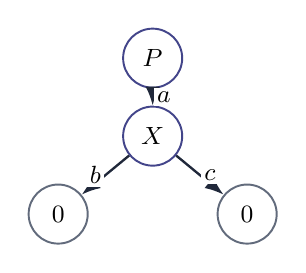
\begin{tikzpicture}[x=1cm,y=.9cm]
        \node[st] (p) at (0,1.1) {$P$}; \node[st] (x) at (0,0) {$X$};
        \node[terminal] (z1) at (-1.2,-1.1) {$0$}; \node[terminal] (z2) at (1.2,-1.1) {$0$};
        \draw[trans] (p)--node[lab,right] {$a$}(x);
        \draw[trans] (x)--node[lab,left] {$b$}(z1);
        \draw[trans] (x)--node[lab,right] {$c$}(z2);
      \end{tikzpicture}
    \end{column}
    \begin{column}{.48\textwidth}\centering
      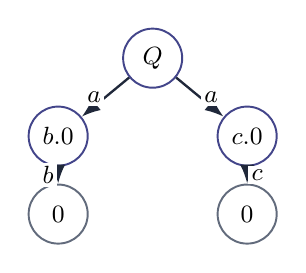
\begin{tikzpicture}[x=1cm,y=.9cm]
        \node[st] (q) at (0,1.1) {$Q$};
        \node[st] (u) at (-1.2,0) {$b.0$}; \node[st] (v) at (1.2,0) {$c.0$};
        \node[terminal] (z1) at (-1.2,-1.1) {$0$}; \node[terminal] (z2) at (1.2,-1.1) {$0$};
        \draw[trans] (q)--node[lab,left] {$a$}(u); \draw[trans] (q)--node[lab,right] {$a$}(v);
        \draw[trans] (u)--node[lab,left] {$b$}(z1); \draw[trans] (v)--node[lab,right] {$c$}(z2);
      \end{tikzpicture}
    \end{column}
  \end{columns}
  \[
    \Tr(P)=\Tr(Q)=\{\varepsilon,a,ab,ac\},\qquad P\not\sim Q.
  \]
  \Takeaway{$P$ satisfies $\langle a\rangle(\langle b\rangle\top\land\langle c\rangle\top)$; $Q$ does not.}
\end{frame}




% 11 -----------------------------------------------------------------
\begin{frame}{Deadlock observations can destroy congruence}
  A \textbf{finite completed trace} ends in a deadlock:
  \[
    \CT(P)=\{w:P\step{w}P'\text{ and }P'\text{ has no outgoing transition}\}.
  \]
  For the preceding $P$ and $Q$, $\CT(P)=\CT(Q)=\{ab,ac\}$.
  \begin{alertblock}{An environment that blocks $c$}
    \[
    \begin{aligned}
      \CT(\blockact{\{c\}}{P})&=\{ab\},\\
      \CT(\blockact{\{c\}}{Q})&=\{a,ab\}.
    \end{aligned}
    \]
    The second process can commit to its $c$-branch and become stuck after $a$.
  \end{alertblock}
  \Takeaway{The ordinary trace languages still agree. Completed-trace equality is not a congruence for blocking.}
  \note{For general infinite-state systems, completed-trace equivalence is often defined to preserve both all traces and completed traces. This example refutes congruence under either convention: the original pair agrees on both. All displayed processes are finite and have no successful-termination predicate.}
\end{frame}

% 12 -----------------------------------------------------------------
\begin{frame}{Why make bisimulation our baseline?}
  \begin{block}{The verification objective}
    Preserve the available continuations after every matched interaction,
    including branching observations and deadlock behaviour.
  \end{block}
  \renewcommand{\arraystretch}{1.45}
  \begin{tabular}{@{}p{.26\textwidth}p{.68\textwidth}@{}}
    \textbf{Logical} & Strong bisimulation preserves HML; on Kripke structures, its label-preserving version preserves CTL$^*$.\\
    \textbf{Algebraic} & It supports substitution under the chosen constructors.\\
    \textbf{Proof-theoretic} & A witness is checked locally by matching transitions; finite-state minimisation uses partition refinement.
  \end{tabular}
  \vspace{2mm}
  \note{Do not say that traces cannot express liveness: 
  equality of infinite state-labelled trace languages preserves LTL, 
  including LTL liveness. 
  Nor do deadlock and compositionality alone uniquely characterise bisimulation: 
  failure/testing semantics offers intermediate alternatives. 
  The chosen baseline reflects this course's branching-time analysis and local proof methods.}
\end{frame}

% 13 -----------------------------------------------------------------
\section{Internal actions and abstraction}
\begin{frame}{Now add internal actions and abstraction}
  Let $\Act=\Sigma\cup\{\tau\}$, with $\tau\notin\Sigma$.\\[1mm]
  $a,b,c\in\Sigma$ are visible; $\alpha\in\Act$ may be internal.\par\vspace{2mm}
  \centering
  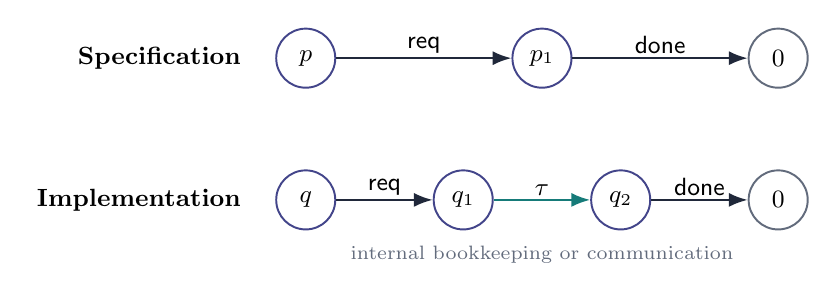
\begin{tikzpicture}[x=1cm,y=1cm]
    \node[anchor=east,font=\small\bfseries] at (-.7,1.35) {Specification};
    \node[st] (p) at (0,1.35) {$p$};
    \node[st] (p1) at (3,1.35) {$p_1$};
    \node[terminal] (p2) at (6,1.35) {$0$};
    \draw[trans] (p)--node[lab,above] {$\mathsf{req}$}(p1);
    \draw[trans] (p1)--node[lab,above] {$\mathsf{done}$}(p2);
    \node[anchor=east,font=\small\bfseries] at (-.7,-.45) {Implementation};
    \node[st] (q) at (0,-.45) {$q$};
    \node[st] (q1) at (2,-.45) {$q_1$};
    \node[st] (q2) at (4,-.45) {$q_2$};
    \node[terminal] (q3) at (6,-.45) {$0$};
    \draw[trans] (q)--node[lab,above] {$\mathsf{req}$}(q1);
    \draw[tauedge] (q1)--node[lab,above] {$\tau$}(q2);
    \draw[trans] (q2)--node[lab,above] {$\mathsf{done}$}(q3);
    \node[font=\scriptsize,text=Muted] at (3,-1.15) {internal bookkeeping or communication};
  \end{tikzpicture}
  \par\vspace{2mm}
  \begin{block}{External behaviour}
    Strong bisimulation distinguishes the initial states because of the internal step.
    We seek a coarser relation that can abstract from this bookkeeping.
  \end{block}
  \note{Spoiler performs req and then the implementation's tau. The specification cannot match that tau strongly. Do not identify hiding with edge deletion: hiding changes labels, retaining the intermediate states and alternatives.}
\end{frame}

% 14 -----------------------------------------------------------------
\begin{frame}{The simplified process algebra with internal actions}
  Let $\Sigma$ contain the visible actions, with $\tau\notin\Sigma$.
  Write
  \[
    \Sigma_\tau=\Sigma\cup\{\tau\},
    \qquad \alpha\in\Sigma_\tau,
    \qquad H\subseteq\Sigma.
  \]

  \begin{block}{Process constructors}
    \renewcommand{\arraystretch}{1.4}
    \begin{tabular}{@{}p{.25\textwidth}p{.69\textwidth}@{}}
      $\nil$
        & No outgoing transitions, not even internal ones.\\
      $\alpha.P$
        & Perform $\alpha$, then behave as $P$.
          In particular, $\tau.P\step{\tau}P$.\\
      $P+Q$
        & The first transition of either summand selects that
          summand and discards the other, even if its label is $\tau$.\\
      $\blockact{H}{P}$
        & Remove transitions labelled in $H$.
          Other transitions, including $\tau$-transitions, remain.\\
      $\hide{H}{P}$ \alert{(new)}
        & Replace labels in $H$ by $\tau$.
          Retain all states and transitions; leave other labels unchanged.


        \end{tabular}
  \end{block}


\end{frame}


\begin{frame}{The simplified process algebra with internal actions}
  Let $\Sigma$ contain the visible actions, with $\tau\notin\Sigma$.
  Write
  \[
    \Sigma_\tau=\Sigma\cup\{\tau\},
    \qquad \alpha\in\Sigma_\tau,
    \qquad H\subseteq\Sigma.
  \]


  \begin{exampleblock}{Blocking prevents an action; hiding conceals it}
    \[
      \blockact{\{a\}}{a.b.\nil}\sim\nil,
      \qquad
      \hide{\{a\}}{a.b.\nil}\sim\tau.b.\nil.
    \]
    After hiding $a$, the process can still reach and perform $b$.
  \end{exampleblock}
\end{frame}



\begin{frame}{Operational rules: an internal step is still a step}
  Throughout, $\alpha\in\Sigma_\tau$ and $H\subseteq\Sigma$.
  The process $\nil$ has no transition rules.

  \begin{block}{Prefix and choice: the same rules for visible and internal actions}
    \[
      \frac{}{\alpha.P\step{\alpha}P}
      \qquad
      \frac{P\step{\alpha}P'}{P+Q\step{\alpha}P'}
      \qquad
      \frac{Q\step{\alpha}Q'}{P+Q\step{\alpha}Q'}.
    \]
  \end{block}

  \begin{block}{Blocking and hiding}
    \[
      \frac{P\step{\alpha}P'}
           {\blockact{H}{P}\step{\alpha}\blockact{H}{P'}}
      \;(\alpha\notin H)
      \qquad
      \frac{P\step{\alpha}P'}
           {\hide{H}{P}\step{h_H(\alpha)}\hide{H}{P'}},
    \]
    where
    \[
      h_H(\alpha)=
      \begin{cases}
        \tau,   & \alpha\in H,\\
        \alpha, & \alpha\notin H.
      \end{cases}
      \qquad\text{In particular, }h_H(\tau)=\tau.
    \]
  \end{block}

\end{frame}



\begin{frame}{Operational rules: an internal step is still a step}
 

  \begin{alertblock}{A silent transition can resolve a choice}
    \[
      \tau.a.\nil+b.\nil\step{\tau}a.\nil,
      \qquad
      \tau.a.\nil+b.\nil\step{b}\nil.
    \]
    Both initial transitions are possible: $\tau$ has no priority.
    If the $\tau$-step occurs, the successor is $a.\nil$,
    \textbf{not} $a.\nil+b.\nil$: the $b$-alternative disappears.
  \end{alertblock}
\end{frame}

% 15 -----------------------------------------------------------------
\begin{frame}{A tempting but inadequate proposal: ignore silent moves}
  Suppose we compare only visible behaviour, allowing internal work before and after it,
  but impose \emph{no obligation} on a purely internal move.
  \[
    P=a.\nil+\tau.\nil,\qquad Q=a.\nil.
  \]
  \centering
  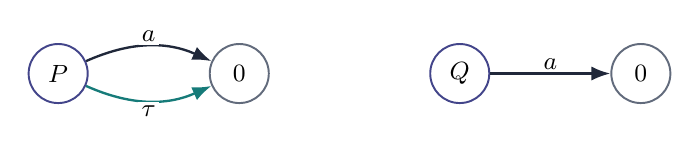
\begin{tikzpicture}[x=1cm,y=1cm]
    \node[st] (p) at (0,0) {$P$}; \node[terminal] (z) at (2.3,0) {$0$};
    \node[st] (q) at (5.1,0) {$Q$}; \node[terminal] (z2) at (7.4,0) {$0$};
    \draw[trans] (p) to[bend left=24] node[lab,above] {$a$}(z);
    \draw[tauedge] (p) to[bend right=24] node[lab,below] {$\tau$}(z);
    \draw[trans] (q)--node[lab,above] {$a$}(z2);
  \end{tikzpicture}
  \par\vspace{3mm}
  \begin{alertblock}{The silent-deadlock problem}
    Both can perform $a$, but only $P$ can silently become stuck \emph{before} $a$.
    The naive proposal ignores that commitment.
  \end{alertblock}
  \Takeaway{Internal transitions must also be matched, even when the matching response may do nothing.}
  \note{A precise failed definition uses the weak-transfer obligation only for visible labels. The symmetric relation {(P,Q),(Q,P),(0,0)} passes that test. This is deliberately not presented as weak bisimulation; the next definition adds the missing obligation. Contracting all internal edges is likewise unsound.}
\end{frame}

% 16 -----------------------------------------------------------------
\section{Weak bisimulation}
\begin{frame}{Weak transitions}
  \begin{block}{Zero or more internal steps}
    \[
      p\silent q\quad\Longleftrightarrow\quad p\step{\tau *}q.
    \]
    In particular, $p\silent p$ always holds.
  \end{block}
  \begin{block}{One visible action, with internal work around it}
    For $a\in\Sigma$,
    \[
      p\wstep{a}q\quad\Longleftrightarrow\quad
      \exists u,v:\ p\silent u\step{a}v\silent q.
    \]
    For uniform notation, define $\;p\wstep{\tau}q\;\Longleftrightarrow\;p\silent q$.
  \end{block}
  \Takeaway{A weak visible move contains exactly one visible action. A weak $\tau$-move may be empty. All matching paths are finite.}
  \Source{Weak-bisimulation notation adapted from the supplied slides; see also \cite{GW96}.}
\end{frame}

% 17 -----------------------------------------------------------------
\begin{frame}{Weak bisimulation}
  \begin{block}{Definition}
    A \textbf{symmetric} relation $R\subseteq S\times S$ is a weak bisimulation if
    \[
      p\,R\,q\ \land\ p\step{\alpha}p'
      \quad\Longrightarrow\quad
      \exists q':\ q\wstep{\alpha}q'\ \land\ p'\,R\,q'
      \qquad(\alpha\in\Act).
    \]
    We write $p\wb q$ if some weak bisimulation relates $p$ and $q$.
  \end{block}
  \centering
  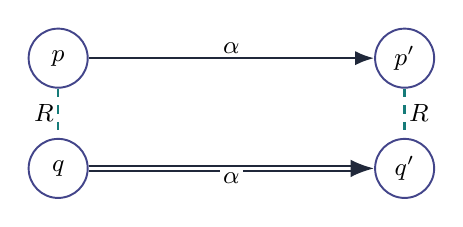
\begin{tikzpicture}[x=1cm,y=1cm]
    \node[st] (p) at (0,1.0) {$p$}; \node[st] (p1) at (4.4,1.0) {$p'$};
    \node[st] (q) at (0,-.4) {$q$}; \node[st] (q1) at (4.4,-.4) {$q'$};
    \draw[trans] (p)--node[lab,above] {$\alpha$}(p1);
    \draw[trans,double,double distance=1pt] (q)--node[lab,below] {$\alpha$}(q1);
    \draw[rel] (p)--node[lab,left] {$R$}(q);
    \draw[rel] (p1)--node[lab,right] {$R$}(q1);
  \end{tikzpicture}
  \par\vspace{1mm}
  {\small Symmetry supplies the same obligation for moves from $q$.}
  \Source{Weak bisimilarity is the greatest weak bisimulation and is an equivalence relation.}
  \note{The union of weak bisimulations is a weak bisimulation. The largest relation is weak bisimilarity and is an equivalence. These facts also follow from the saturation construction in the backup slides.}
\end{frame}


% ----------------------------------------------------------------------
\begin{frame}{Weak Hennessy--Milner logic}
  Recall
  \[
    p\Rightarrow q
    \quad\Longleftrightarrow\quad
    p\step{\tau *}q,
  \]
  and, for $a\in\Sigma$,
  \[
    p\xRightarrow{a}q
    \quad\Longleftrightarrow\quad
    p\step{\tau *}\step{a}\step{\tau *}q.
  \]

  \begin{block}{Weak modalities}
    \[
      \varphi ::= \top
      \mid \neg\varphi
      \mid \varphi\land\psi
      \mid \langle\!\langle\alpha\rangle\!\rangle\varphi,
      \qquad \alpha\in\Sigma\cup\{\tau\}.
    \]
    \[
      p\models\langle\!\langle\alpha\rangle\!\rangle\varphi
      \quad\Longleftrightarrow\quad
      \exists q:\;
      p\xRightarrow{\alpha}q
      \land q\models\varphi .
    \]
    For $\alpha=\tau$, we put $\xRightarrow{\tau}=\Rightarrow$,
    so zero or more internal steps are allowed.
  \end{block}

  \Takeaway{The logic observes the endpoint of a weak transition,
  but not the states crossed by its internal part.}
\end{frame}


% ----------------------------------------------------------------------
\begin{frame}{Weak HML characterizes weak bisimulation}
  \begin{block}{Theorem}
    For finite LTSs,
    \[
      p\approx_{\mathrm w}q
      \quad\Longleftrightarrow\quad
      \forall\varphi\in\mathrm{WHML}:
      \bigl(p\models\varphi\iff q\models\varphi\bigr).
    \]
  \end{block}



  \begin{block}{Why? Saturate the transition system}
    Construct $\mathrm{Sat}(T)$ by putting
    \[
      p\step{a}_{\mathrm w}q
      \quad\Longleftrightarrow\quad
      p\xRightarrow{a}q,  \text{ and }
    \]
    \[
      p\step{\tau}_{\mathrm w}q
      \quad\Longleftrightarrow\quad
      p\Rightarrow q.
    \]
    Then
    \[
      p\approx_{\mathrm w}q\text{ in }T
      \quad\Longleftrightarrow\quad
      p\sim q\text{ in }\mathrm{Sat}(T).
    \]
    Apply the ordinary Hennessy--Milner theorem to $\mathrm{Sat}(T)$.
  \end{block}

  \Takeaway{Weak bisimulation is ordinary bisimulation after forgetting
  the internal structure of finite silent computations.}
  \Source{Hennessy--Milner; De Nicola--Vaandrager.}
\end{frame}


% ----------------------------------------------------------------------
\begin{frame}{What if the logic can inspect a silent computation?}
  Weak HML sees only
  \[
      p \xRightarrow{a} q.
  \]
  It cannot ask what remains possible \emph{while} the silent preparation
  for $a$ is taking place.

  \begin{block}{A CTL-style ``until'' operator}
    Introduce
    \[
      \varphi\langle a\rangle\psi
    \]
    with the semantics
    \[
    p\models\varphi\langle a\rangle\psi
    \]
    iff there exist
    \[
      p=p_0\step{\tau}p_1\step{\tau}\cdots
      \step{\tau}p_n\step{a}q
    \]
    such that
    \[
      p_i\models\varphi\quad(0\leq i\leq n),
      \qquad q\models\psi.
    \]
  \end{block}

  \Takeaway{This is an ``until $a$ happens'' modality:
  it observes properties of the intermediate silent states.}

  \note{This is the essential operator of Hennessy--Milner Logic with Until,
  HMLU. I would call it CTL-style rather than ``weak CTL'', because
  ``CTL over the saturated LTS'' would have different semantics.}
\end{frame}


% ----------------------------------------------------------------------
\begin{frame}{Until can distinguish weakly bisimilar processes}
  Consider
  \[
    R=\tau.a.\nil+b.\nil,
    \qquad
    S=a.\nil+\tau.a.\nil+b.\nil.
  \]

  \begin{columns}[T,onlytextwidth]
    \begin{column}{.46\textwidth}\centering
      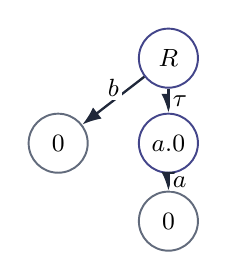
\begin{tikzpicture}[x=1cm,y=.9cm]
        \node[st] (r) at (0,1.2) {$R$};
        \node[st] (r1) at (0,0) {$a.0$};
        \node[terminal] (z1) at (0,-1.1) {$0$};
        \node[terminal] (z2) at (-1.4,0) {$0$};

        \draw[trans] (r)--node[lab,right] {$\tau$}(r1);
        \draw[trans] (r1)--node[lab,right] {$a$}(z1);
        \draw[trans] (r)--node[lab,above] {$b$}(z2);
      \end{tikzpicture}
    \end{column}

    \begin{column}{.50\textwidth}\centering
      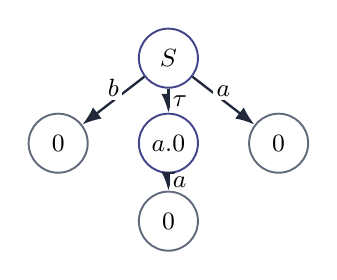
\begin{tikzpicture}[x=1cm,y=.9cm]
        \node[st] (s) at (0,1.2) {$S$};
        \node[st] (s1) at (0,0) {$a.0$};
        \node[terminal] (za) at (1.4,0) {$0$};
        \node[terminal] (zb) at (-1.4,0) {$0$};
        \node[terminal] (z1) at (0,-1.1) {$0$};

        \draw[trans] (s)--node[lab,right] {$\tau$}(s1);
        \draw[trans] (s1)--node[lab,right] {$a$}(z1);
        \draw[trans] (s)--node[lab,above] {$a$}(za);
        \draw[trans] (s)--node[lab,above] {$b$}(zb);
      \end{tikzpicture}
    \end{column}
  \end{columns}

  \[
      R\approx_{\mathrm w}S.
  \]

  But let
  \[
      \chi=
      \bigl(\langle\!\langle b\rangle\!\rangle\top\bigr)
      \langle a\rangle\top.
  \]
  Then
  \[
      S\models\chi,
      \qquad
      R\not\models\chi.
  \]

  \Takeaway{Weak bisimulation forgets too much for an until operator
  that inspects the internal path.}
\end{frame}


% ----------------------------------------------------------------------
\begin{frame}{What exactly does the formula observe?}
  \[
      \chi=
      \bigl(\langle\!\langle b\rangle\!\rangle\top\bigr)
      \langle a\rangle\top.
  \]

  \begin{block}{$S\models\chi$}
    $S$ may perform $a$ immediately:
    \[
       S\step{a}0.
    \]
    Before $a$ happens, we are still in $S$, where $b$ is possible.
  \end{block}

  \begin{alertblock}{$R\not\models\chi$}
    Every execution of $a$ has to start with
    \[
       R\step{\tau}a.0\step{a}0.
    \]
    After the silent step the $b$-alternative has disappeared:
    \[
       a.0\not\models
       \langle\!\langle b\rangle\!\rangle\top.
    \]
  \end{alertblock}

  \Takeaway{The difference is not the visible trace.
  It is \emph{when a branching possibility disappears}.}
\end{frame}


% ----------------------------------------------------------------------
\begin{frame}{Branching bisimulation}
  \begin{block}{Definition}
    A symmetric relation $R$ is a \textbf{branching bisimulation} if
    $p\,R\,q$ and
    \[
       p\step{\alpha}p'
    \]
    imply either
    \[
       \alpha=\tau
       \quad\text{and}\quad p'\,R\,q,
    \]
    or there exist $q_0,q'$ such that
    \[
       q\Rightarrow q_0\step{\alpha}q',
       \qquad
       p\,R\,q_0,
       \qquad
       p'\,R\,q'.
    \]
  \end{block}

  \begin{center}
    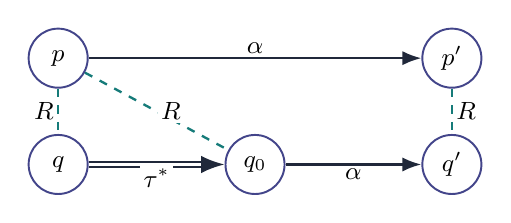
\begin{tikzpicture}[x=1.25cm,y=.9cm]
      \node[st] (p)  at (0,1) {$p$};
      \node[st] (pp) at (4,1) {$p'$};
      \node[st] (q)  at (0,-.5) {$q$};
      \node[st] (q0) at (2,-.5) {$q_0$};
      \node[st] (qp) at (4,-.5) {$q'$};

      \draw[trans] (p)--node[lab,above] {$\alpha$}(pp);
      \draw[trans,double,double distance=1pt]
         (q)--node[lab,below] {$\tau^*$}(q0);
      \draw[trans] (q0)--node[lab,below] {$\alpha$}(qp);
      \draw[rel] (p)--node[lab,left] {$R$}(q);
      \draw[rel] (p)--node[lab,right] {$R$}(q0);
      \draw[rel] (pp)--node[lab,right] {$R$}(qp);
    \end{tikzpicture}
  \end{center}

  \Takeaway{Silent preparation may be ignored only while the original
  branching situation is preserved.}
\end{frame}


% ----------------------------------------------------------------------
\begin{frame}{Weak versus branching bisimulation}
  For the previous processes,
  \[
      R=\tau.a.0+b.0,
      \qquad
      S=a.0+\tau.a.0+b.0,
  \]
  we have
  \[
      R\approx_{\mathrm w}S,
      \qquad
      R\not\approx_{\mathrm b}S.
  \]

  \begin{block}{Why does branching bisimulation fail?}
    Consider the direct transition
    \[
       S\step{a}0.
    \]
    The only way $R$ can prepare an $a$ is
    \[
       R\step{\tau}a.0\step{a}0.
    \]
    Branching bisimulation would require
    \[
       S\approx_{\mathrm b}a.0
    \]
    immediately before the matching $a$.
    This is impossible: $S$ still offers $b$, while $a.0$ does not.
  \end{block}

  \Takeaway{Branching bisimulation remembers which choices survive
  during an internal computation.}
\end{frame}


% ----------------------------------------------------------------------
\begin{frame}{Hennessy--Milner logic with Until}
  \begin{block}{HMLU}
    \[
      \varphi ::=
      \top
      \mid\neg\varphi
      \mid\varphi\land\psi
      \mid\varphi\langle\alpha\rangle\psi .
    \]
    The last operator requires an internal path
    \[
      p=p_0\step{\tau}\cdots\step{\tau}p_n
      \step{\alpha}q
    \]
    such that every $p_i$ satisfies $\varphi$ and $q$ satisfies $\psi$.
  \end{block}

  \begin{block}{Theorem}
    For finite LTSs,
    \[
       p\approx_{\mathrm b}q
       \quad\Longleftrightarrow\quad
       p\text{ and }q\text{ satisfy the same HMLU formulas}.
    \]
  \end{block}

  \[
      \underbrace{\text{weak HML}}_{\text{endpoint only}}
      \quad\leadsto\quad
      \approx_{\mathrm w}
      \qquad
      \underbrace{\text{HMLU}}_{\text{inspect silent prefix}}
      \quad\leadsto\quad
      \approx_{\mathrm b}.
  \]

  \Takeaway{The extra logical power of ``until'' corresponds exactly
  to preservation of branching during silent computation.}
  \Source{De Nicola and Vaandrager, JACM 42(2), 1995.}
\end{frame}


% ----------------------------------------------------------------------
\begin{frame}{Connection with CTL without the next operator}
  HMLU already gives the cleanest action-based characterization.
  There is also a direct connection with CTL.

  \begin{block}{Translate an LTS to a state-labelled system}
    Keep original states and label them by a fresh proposition $\bot$.
    Replace every visible transition
    \[
        p\step{a}q
    \]
    by
    \[
        p\longrightarrow [p,a,q]\longrightarrow q,
    \]
    where the intermediate state is labelled by $a$.
    Silent transitions $p\step{\tau}q$ remain direct edges.
  \end{block}

  \begin{block}{Theorem for finite LTSs}
    Under the divergence-blind interpretation,
    \[
      p\approx_{\mathrm b}q
      \quad\Longleftrightarrow\quad
      p,q\text{ satisfy the same }\mathrm{CTL}^{*}\!-\!X
      \text{ formulas}.
    \]
    In fact, $\mathrm{CTL}-X$ already induces the same equivalence.
  \end{block}

  \Takeaway{Removing $X$ makes finite stuttering invisible,
  while Until still observes whether properties remain true
  throughout the stuttering segment.}
\end{frame}


% ----------------------------------------------------------------------
\begin{frame}{Infinite silence is a separate question}
  Consider
  \[
  \begin{array}{c@{\qquad\qquad}c}
    p\step{a}0
    &
    q\step{a}0,\qquad q\step{\tau}q .
  \end{array}
  \]

  \begin{block}{Ordinary weak and branching bisimulation}
    \[
       p\approx_{\mathrm w}q,
       \qquad
       p\approx_{\mathrm b}q.
    \]
    The $\tau$-loop can be ignored forever.
  \end{block}

  \begin{alertblock}{But there is an observable design question}
    $q$ admits an infinite internal computation
    \[
       q\step{\tau}q\step{\tau}q\step{\tau}\cdots,
    \]
    while $p$ does not.
  \end{alertblock}

  If this distinction matters, use a
  \textbf{divergence-preserving} version of the equivalence
  (and a corresponding divergence-sensitive logic).

  \Takeaway{Two independent questions arise:
  what may finite silent computation forget, and whether infinite silence matters.}
\end{frame}


% ----------------------------------------------------------------------
\begin{frame}{Weak and branching bisimilarity are not congruences}
  Both equivalences abstract from an initial finite silent computation:
  \[
       \tau.0\approx_{\mathrm w}0,
       \qquad
       \tau.0\approx_{\mathrm b}0.
  \]

  Now put the processes in the choice context
  \[
       C[-]=a.0+[-].
  \]

  Then
  \[
      C[\tau.0]=a.0+\tau.0,
      \qquad
      C[0]=a.0+0.
  \]

  But
  \[
      a.0+\tau.0\not\approx_{\mathrm w}a.0+0.
  \]
  The left process can silently choose the second branch and deadlock,
  while the right process cannot.

  Hence also
  \[
      a.0+\tau.0\not\approx_{\mathrm b}a.0+0.
  \]

  \Takeaway{The problem is at the root:
  an initial silent step may resolve an external choice.}
\end{frame}


% ----------------------------------------------------------------------
\begin{frame}{Rooted weak bisimilarity}
  To recover substitution under choice, treat the first move more strictly.

  Define
  \[
  q\xRightarrow{\widehat{\alpha}}q'=
  \begin{cases}
    q\Rightarrow\step{a}\Rightarrow q',
       & \alpha=a\in\Sigma,\\[1mm]
    q\Rightarrow\step{\tau}\Rightarrow q',
       & \alpha=\tau.
  \end{cases}
  \]
  Notice that a root $\tau$ must now be matched by
  \textbf{at least one} $\tau$.

  \begin{block}{Rooted weak bisimilarity}
    \[
      p\approx_{\mathrm{rw}}q
    \]
    iff every initial
    \[
      p\step{\alpha}p'
    \]
    can be matched by
    \[
      q\xRightarrow{\widehat{\alpha}}q'
      \qquad\text{with}\qquad
      p'\approx_{\mathrm w}q',
    \]
    and symmetrically.
  \end{block}

  Thus
  \[
     \tau.0\not\approx_{\mathrm{rw}}0.
  \]

  \Takeaway{After the root has been matched, ordinary weak
  bisimilarity is sufficient again.}
\end{frame}


% ----------------------------------------------------------------------
\begin{frame}{Rooted branching bisimilarity}
  For branching bisimulation the standard root condition is even cleaner.

  \begin{block}{Definition}
    \[
       p\approx_{\mathrm{rb}}q
    \]
    iff every initial transition
    \[
       p\step{\alpha}p'
    \]
    can be matched by an actual transition
    \[
       q\step{\alpha}q'
    \]
    such that
    \[
       p'\approx_{\mathrm b}q',
    \]
    and symmetrically.
  \end{block}

  \begin{block}{Compositional role}
    The rooted variants repair the failure under nondeterministic choice.
    For the standard CCS-style operators they give the corresponding
    congruences.
  \end{block}

  \Takeaway{Rootedness and branching preservation solve different problems:
  branching controls what may happen \emph{inside} a silent computation;
  rootedness controls how a component may be used by its environment.}
\end{frame}


% ----------------------------------------------------------------------
\begin{frame}{What $\tau$ adds to the picture}
  \begin{center}
  \renewcommand{\arraystretch}{1.45}
  \begin{tabular}{@{}lll@{}}
    \textbf{Observation} &
    \textbf{Logic} &
    \textbf{Equivalence}\\
    \hline
    every transition &
    HML &
    strong bisimulation\\

    endpoints of silent computations &
    weak HML &
    weak bisimulation\\

    branching preserved during silence &
    HML with Until &
    branching bisimulation\\

    finite stuttering in branching time &
    CTL$^{*}{-}X$ &
    branching bisimulation\\
  \end{tabular}
  \end{center}

  \vspace{4mm}

  Two additional refinements answer independent questions:
  \[
      \text{divergence preservation}
      \qquad\text{and}\qquad
      \text{rootedness / congruence}.
  \]

  \Takeaway{There is no single way to ``ignore $\tau$'':
  the equivalence depends on what the observer is allowed to see.}
\end{frame}

% 18 -----------------------------------------------------------------
\begin{frame}{First example: an internal delay}
  \[
    P=a.\nil,\qquad Q=\tau.a.\nil.
  \]
  \centering
  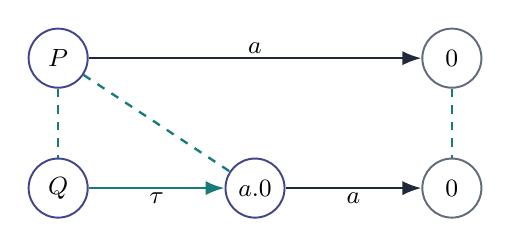
\begin{tikzpicture}[x=1cm,y=1cm]
    \node[st] (p) at (0,1.05) {$P$}; \node[terminal] (p0) at (5,1.05) {$0$};
    \node[st] (q) at (0,-.6) {$Q$}; \node[st] (q1) at (2.5,-.6) {$a.0$};
    \node[terminal] (q0) at (5,-.6) {$0$};
    \draw[trans] (p)--node[lab,above] {$a$}(p0);
    \draw[tauedge] (q)--node[lab,below] {$\tau$}(q1);
    \draw[trans] (q1)--node[lab,below] {$a$}(q0);
    \draw[rel] (p)--(q); \draw[rel] (p)--(q1); \draw[rel] (p0)--(q0);
  \end{tikzpicture}
  \par\vspace{1mm}
  \uncover<2->{\Takeaway{$P\wb Q$, but $P\not\sim Q$. The $\tau$-step of $Q$ can be matched by $P$ doing nothing.}}
  \note{The two displayed states named a.0/P have identical behaviour; the dotted links show a possible witness across disjoint copies. All displayed zero states are deadlocks.}
\end{frame}

% 19 -----------------------------------------------------------------
\begin{frame}{Weak bisimulation detects silent deadlock}
  Return to $P=a.\nil+\tau.\nil$ and $Q=a.\nil$.
  \begin{block}{The missing obligation is now present}
    If $P\,R\,Q$ and $P\step{\tau}\nil$, we need
    \[
      Q\silent Q'\quad\text{and}\quad\nil\,R\,Q'.
    \]
    $Q$ has no internal move, so $Q'=Q$.
    But $Q$ can perform $a$, and $\nil$ cannot match it.
  \end{block}
  Therefore $P\notwb Q$.
  \begin{exampleblock}{What is intentionally ignored}
    $\tau.\nil\wb\nil$: finite internal work leading only to inaction adds no visible possibility.

  \end{exampleblock}
  \Takeaway{Ignore the duration of finite internal work, not its effect on the available continuations.}
\end{frame}

% 20 -----------------------------------------------------------------
\section{Branching bisimulation}
\begin{frame}{Weak matching may pass over a choice}
  \centering
  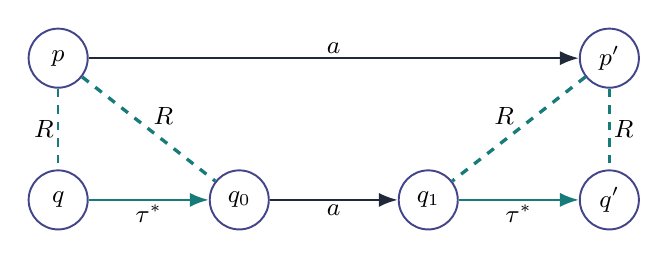
\begin{tikzpicture}[x=1cm,y=1cm]
    \node[st] (p) at (0,1.3) {$p$}; \node[st] (pp) at (7,1.3) {$p'$};
    \node[st] (q) at (0,-.5) {$q$}; \node[st] (q0) at (2.3,-.5) {$q_0$};
    \node[st] (q1) at (4.7,-.5) {$q_1$}; \node[st] (qq) at (7,-.5) {$q'$};
    \draw[trans] (p)--node[lab,above] {$a$}(pp);
    \draw[tauedge] (q)--node[lab,below] {$\tau^*$}(q0);
    \draw[trans] (q0)--node[lab,below] {$a$}(q1);
    \draw[tauedge] (q1)--node[lab,below] {$\tau^*$}(qq);
    \draw[rel] (p)--node[lab,left] {$R$}(q);
    \draw[rel] (pp)--node[lab,right] {$R$}(qq);
    \uncover<2->{\draw[rel,line width=1.2pt] (p)--node[lab,above right] {$R$}(q0);
      \draw[rel,line width=1.2pt] (pp)--node[lab,above left] {$R$}(q1);}
  \end{tikzpicture}
  \par\vspace{4mm}
  \begin{block}{Weak bisimulation}
    Requires related endpoints; no explicit obligations at $q_0$ and $q_1$.
  \end{block}
  \uncover<2->{\Takeaway{Branching bisimulation also preserves the choices \emph{around} the matching visible action. We use an equivalent definition with no trailing silent path.}}
  \Source{Adapted matching diagram from \cite{GW96}; the next slide uses the formulation of \cite{GLT09}.}
\end{frame}

% 21 -----------------------------------------------------------------
\begin{frame}{Branching bisimulation: definition}
  Write $u\optstep{\alpha}v$ for a single $\alpha$-step, or for $u=v$ when $\alpha=\tau$.
  \begin{block}{Definition}
    A symmetric relation $R$ is a \textbf{branching bisimulation} if
    $p\,R\,q$ and $p\step{\alpha}p'$ imply that there exist $q_0,q'$ with
    \[
      q\silent q_0\optstep{\alpha}q',
      \qquad \boxed{p\,R\,q_0},\qquad p'\,R\,q'.
    \]
    We write $p\bb q$ if some branching bisimulation relates them.
  \end{block}
  \begin{itemize}\setlength\itemsep{2mm}
    \item Before the matching action, $q_0$ must still represent $p$.
    \item Immediately afterwards, $q'$ must represent $p'$.
    \item A $\tau$-step may be ignored only when the required states remain related.
  \end{itemize}
  \Source{\cite[Definition 2.1]{GLT09}. Branching bisimilarity is an equivalence relation.}
  \note{This is the optional-final-step relational definition from GLT09, which induces standard branching bisimilarity. Do not insist that every tau-transition must be inert. For the largest relation, the stuttering property ensures that the preparatory tau path stays in the source equivalence class.}
\end{frame}

% 22 -----------------------------------------------------------------
\begin{frame}{Weak, but not branching, bisimilar}
  \[
    X=b.\nil+\tau.C,\quad C=c.\nil,\qquad
    P=a.X,\quad Q=a.X+a.C.
  \]
  \centering
  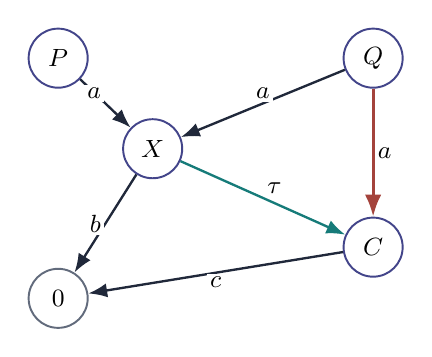
\begin{tikzpicture}[x=1cm,y=1cm]
    \node[st] (p) at (-2,1.05) {$P$};
    \node[st] (q) at (2,1.05) {$Q$};
    \node[st] (x) at (-.8,-.1) {$X$};
    \node[st] (c) at (2,-1.35) {$C$};
    \node[terminal] (z) at (-2,-2.0) {$0$};
    \draw[trans] (p)--node[lab,above left] {$a$}(x);
    \draw[trans] (q)--node[lab,above] {$a$}(x);
    \draw[newedge] (q)--node[lab,right] {$a$}(c);
    \draw[tauedge] (x)--node[lab,above right] {$\tau$}(c);
    \draw[trans] (x)--node[lab,left] {$b$}(z);
    \draw[trans] (c)--node[lab,below] {$c$}(z);
  \end{tikzpicture}
  \par\vspace{1mm}
  \Takeaway{$P\wb Q$, but $P\notbb Q$: the additional transition bypasses $X$, where $b$ is still possible.}
  \note{This is a compact instance of the standard weak tau-law a.(B+tau.C)+a.C approximately a.(B+tau.C). Share X, C and 0 between the two roots, so the weak witness consists of identity pairs plus (P,Q) and its converse.}
\end{frame}

% 23 -----------------------------------------------------------------
\begin{frame}{The separating example: why the relations differ}
  \[
    P=a.X,\quad Q=a.X+a.C,\quad X=b.\nil+\tau.C,\quad C=c.\nil.
  \]
  \begin{columns}[T,onlytextwidth]
    \begin{column}{.48\textwidth}
      \begin{exampleblock}{Weak: $P\wb Q$}
        Match the additional move $Q\step{a}C$ by
        \[
          P\step{a}X\step{\tau}C.
        \]
        Other moves match directly.\\[1mm]
        A witness is
        \[
          R=\Id\cup\{(P,Q),(Q,P)\}.
        \]
      \end{exampleblock}
    \end{column}
    \begin{column}{.48\textwidth}
      \begin{alertblock}{Branching: $P\notbb Q$}
        $P$ has no initial $\tau$-step. Matching $Q\step{a}C$ must therefore use
        \[
          P\step{a}X.
        \]
        This requires $X\bb C$, but only $X$ can perform $b$.
      \end{alertblock}
    \end{column}
  \end{columns}
  \Takeaway{Weak matching may combine the $a$-step with discarding $b$. Branching matching cannot.}
\end{frame}

% 24 -----------------------------------------------------------------
\begin{frame}{Why prefer branching bisimulation?}
  For a visible step $p\step{a}p'$, a branching response can be chosen as
  \[
    \begin{gathered}
      q=q_0\step{\tau}q_1\step{\tau}\cdots\step{\tau}q_k\step{a}q',\\[1mm]
      \boxed{p\bb q_i\quad(0\leq i\leq k)},\qquad p'\bb q'.
    \end{gathered}
  \]
  \begin{block}{Internal preparation stays in one abstract state}
    Every $q_i$ represents $p$. Immediately after the matching visible step,
    $q'$ represents $p'$.
  \end{block}
  \begin{exampleblock}{Contrast with weak matching}
    Only the endpoints must be related. Internal preparation and completion
    may pass through other behaviours.
  \end{exampleblock}
  \Takeaway{Branching equivalence preserves more intermediate structure. Divergence preservation and rootedness remain separate requirements.}
  \vspace{-2mm}\Source{Branching transfer and the stuttering property: \cite{GW96,GLT09}.}
  \note{For the largest branching equivalence, both ends of the preparatory path are equivalent to p. The stuttering property puts every intermediate state in that class. Do not present the bare endpoint stuttering property alone as a separator from weak bisimilarity: the extra transfer obligations are decisive. Weak bisimulation remains a legitimate coarser observation regime.}
\end{frame}

% 25 -----------------------------------------------------------------
\begin{frame}{Three equivalences, three levels of abstraction}
  \[
    {\sim}\ \subsetneq\ {\approx_{\mathrm b}}\ \subsetneq\ {\approx_{\mathrm w}}.
  \]
  \vspace{3mm}
  \renewcommand{\arraystretch}{1.6}
  \begin{tabular}{@{}p{.27\textwidth}p{.67\textwidth}@{}}
    \textbf{Strong} & Match one transition by one transition.\\
    \textbf{Branching} & Abstract from internal steps while preserving branching during matching.\\
    \textbf{Weak} & Match transitions by weak paths with related endpoints.
  \end{tabular}
  \vspace{2mm}
  \begin{block}{Witnesses for strictness}
    $a.\nil\bb\tau.a.\nil$, but they are not strongly bisimilar.\\[1mm]
    The previous $P,Q$ are weakly, but not branching, bisimilar.
  \end{block}
  \Source{On LTSs without $\tau$-transitions, all three notions coincide. See \cite{GW96}.}
  \note{Branching implies weak directly: the branching response is a legal weak response. For an optional tau final step this is still a tau-star path. No claim about a partial-order or true-concurrency semantics is being made.}
\end{frame}

% 26 -----------------------------------------------------------------
\section{Divergence}
\begin{frame}{Divergence: silent activity may continue forever}
  \begin{block}{Definition}
    A state $p$ \textbf{diverges} if there is an infinite execution
    \[
      p=p_0\step{\tau}p_1\step{\tau}p_2\step{\tau}\cdots.
    \]
  \end{block}
  \centering
  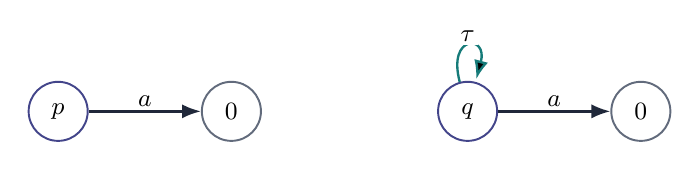
\begin{tikzpicture}[x=1cm,y=1cm]
    \node[st] (p) at (0,0) {$p$}; \node[terminal] (z1) at (2.2,0) {$0$};
    \node[st] (q) at (5.2,0) {$q$}; \node[terminal] (z2) at (7.4,0) {$0$};
    \draw[trans] (p)--node[lab,above] {$a$}(z1);
    \draw[trans] (q)--node[lab,above] {$a$}(z2);
    \draw[tauedge] (q) edge[loop above] node[lab] {$\tau$} (q);
  \end{tikzpicture}
  \par\vspace{2mm}
  \uncover<2->{\Takeaway{$p\bb q$, yet only $q$ has an infinite execution avoiding $a$.}}
  \Source{For maximal executions, with no fairness assumption. Infinite activity is not a deadlock.}
\end{frame}

% 27 -----------------------------------------------------------------
\begin{frame}{Finite silence, deadlock, and infinite silence}
  Let $D$ have only the self-loop $D\step{\tau}D$.
  \begin{block}{Ordinary weak and branching bisimilarity}
    \[
      \nil\bb\tau.\nil\bb D.
    \]
    All three have no visible behaviour, but only $D$ has infinite internal activity.
  \end{block}
  \begin{exampleblock}{Divergence-preserving branching bisimilarity}
    Add an obligation to match infinite internal activity within related behaviour.
    Then
    \[
      \nil\dbb\tau.\nil,\qquad \nil\notdbb D.
    \]
  \end{exampleblock}
  \Takeaway{Divergence preservation distinguishes infinite activity from finite silence. It does not make every internal step observable.}
  \Source{\cite{GLT09}. No fairness assumption is implicit; the exact divergence clause is in the appendix.}
  \note{A deadlock has no outgoing transition. An internal loop is not a deadlock, even though it may provide no visible progress. Ordinary weak and branching equivalence ignore this distinction in the pure-loop example. The previous example with an a-exit explains why this matters for inevitable response. Do not claim preservation of arbitrary CTL formulas or arbitrary fairness assumptions.}
\end{frame}

% 28 -----------------------------------------------------------------
\section{Rooted relations}
\begin{frame}{Ordinary weak equivalences fail under choice}
  \[
    P=\tau.a.\nil\bb a.\nil=Q,\qquad C[-]=[-]+b.\nil.
  \]
  \begin{columns}[T,onlytextwidth]
    \begin{column}{.49\textwidth}\centering
      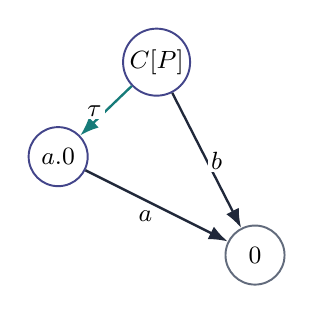
\begin{tikzpicture}[x=1cm,y=1cm]
        \node[st] (p) at (0,1.0) {$C[P]$};
        \node[st] (a) at (-1.25,-.2) {$a.0$};
        \node[terminal] (z) at (1.25,-1.45) {$0$};
        \draw[tauedge] (p)--node[lab,left] {$\tau$}(a);
        \draw[trans] (p)--node[lab,right] {$b$}(z);
        \draw[trans] (a)--node[lab,below left] {$a$}(z);
      \end{tikzpicture}
    \end{column}
    \begin{column}{.49\textwidth}\centering
      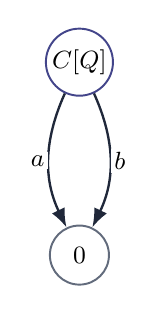
\begin{tikzpicture}[x=1cm,y=1cm]
        \node[st] (q) at (0,1.0) {$C[Q]$};
        \node[terminal] (z) at (0,-1.45) {$0$};
        \draw[trans] (q) to[bend right=25] node[lab,left] {$a$} (z);
        \draw[trans] (q) to[bend left=25] node[lab,right] {$b$} (z);
      \end{tikzpicture}
    \end{column}
  \end{columns}
  \uncover<2->{\Takeaway{$C[P]\notwb C[Q]$, hence also $C[P]\notbb C[Q]$. The left process can silently discard $b$; the right process cannot.}}
  \Source{The weak-choice counterexample from the supplied slides, made explicit.}
\end{frame}

% 29 -----------------------------------------------------------------
\begin{frame}{The coarsest congruence contained in an equivalence}
  Starting with an equivalence $\approx$, define
  \[
    P\approx^{\mathrm{ctx}}Q
    \quad\Longleftrightarrow\quad
    \forall C[-]:\ C[P]\approx C[Q].
  \]
  \begin{block}{Why this is the desired repair}
    \begin{itemize}\setlength\itemsep{2mm}
      \item The identity context gives $\approx^{\mathrm{ctx}}\,\subseteq\,\approx$.
      \item Composing contexts shows that $\approx^{\mathrm{ctx}}$ is a congruence.
      \item Every congruence contained in $\approx$ is contained in $\approx^{\mathrm{ctx}}$.
    \end{itemize}
  \end{block}
  \Takeaway{Root conditions give a local characterisation, avoiding quantification over all contexts.}
  \Source{For the usual CCS setting, root conditions provide such characterisations; see \cite{MCS}.}
  \note{The claim that contextual refinement is an equivalence is pointwise inherited from the base equivalence. Closure of our one-hole contexts under composition proves compatibility. 'Coarsest' means largest as a relation among congruences contained in the base equivalence.}
\end{frame}

% 30 -----------------------------------------------------------------
\begin{frame}{Rooted branching bisimilarity}
  \begin{block}{Definition}
    $P\rbb Q$ if every transition $P\step{\alpha}P'$ has a match
    \[
      Q\step{\alpha}Q'\quad\text{with}\quad P'\bb Q',
    \]
    and conversely, for every $\alpha\in\Act$.
  \end{block}
  \Takeaway{Match the initial step \textbf{strictly}, including $\tau$; compare successors by \textbf{ordinary branching bisimilarity}.}
  \[
    \tau.a.\nil\notrbb a.\nil,
    \qquad
    a.\tau.b.\nil\rbb a.b.\nil.
  \]
  {\small\textcolor{Warn}{Do not require rooted equivalence of the successors:} that would impose strong-style matching at every step.}
  \Source{Root conditions: \cite{MCS,GLS20}.}
\end{frame}

% 31 -----------------------------------------------------------------
\begin{frame}{Rooted weak bisimilarity: a different root condition}
  \begin{block}{Definition: observational congruence}
    $P\rwb Q$ if every $P\step{\alpha}P'$ can be matched by
    \[
      Q\silent Q_0\step{\alpha}Q_1\silent Q'
      \quad\text{with}\quad P'\wb Q',
    \]
    and symmetrically, for all $\alpha\in\Act$.
  \end{block}
  \begin{alertblock}{The middle step is compulsory, also for $\alpha=\tau$}
    Matching an initial $\tau$ requires at least one $\tau$-transition: $\tau^+$, not merely $\tau^*$.
  \end{alertblock}
  \renewcommand{\arraystretch}{1.45}
  \begin{tabular}{@{}ll@{}}
    Rooted branching: & one initial step; branching-equivalent successors.\\
    Rooted weak: & a nonempty matching weak path; weak-equivalent successors.
  \end{tabular}
  \Source{\cite{MCS}. Both are congruences for the constructors used in the lecture.}
\end{frame}

% 32 -----------------------------------------------------------------
\begin{frame}{Rootedness repairs the choice problem}
  \begin{block}{Theorem}
    Rooted branching and rooted weak bisimilarity are congruences for prefix, choice, blocking, and hiding.
  \end{block}
  \textbf{Choice case.} Assume $P\rbb Q$ and consider $P+R$ and $Q+R$.
  \begin{itemize}\setlength\itemsep{2.5mm}
    \item If $P+R\step{\alpha}P'$ uses $P$, rootedness provides
      $Q\step{\alpha}Q'$ with $P'\bb Q'$. Thus $Q+R$ has the required \emph{single} matching step.
    \item If the move uses $R$, use the identical step of $R$ on the other side.
  \end{itemize}
  \Takeaway{Once the first transition has resolved the choice, ordinary branching equivalence suffices for the derivatives.}
  \Source{\cite{MCS}. For rooted weak equivalence, a nonempty response also resolves the outer choice; a zero-step response would not.}
  \note{For prefix, use P approximately_b Q, implied by rootedness. For parallel, the immediate step is either a component step or a synchronisation, and the derivative pair is branching equivalent by compatibility of branching equivalence with parallel. Restriction and hiding preserve the matching label, and the derivative pair remains branching equivalent.}
\end{frame}

% 33 -----------------------------------------------------------------
\begin{frame}{Rootedness and divergence solve different problems}
  \renewcommand{\arraystretch}{1.55}
  \begin{tabular}{@{}p{.26\textwidth}p{.68\textwidth}@{}}
    \textbf{Rootedness} & Protects initial branching when a component is placed in a context.\\
    \shortstack[l]{\textbf{Divergence}\\\textbf{preservation}} & Prevents infinite internal activity from being erased by equivalence.
  \end{tabular}
  \vspace{3mm}
  Let $D$ have only the self-loop $D\step{\tau}D$. Then
  \[
    a.\nil\rbb a.D,
    \qquad\text{but}\qquad a.\nil\notdbb a.D.
  \]
  \uncover<2->{\begin{block}{The other direction also fails}
    \[
      a.\nil\dbb\tau.a.\nil,
      \qquad a.\nil\notrbb\tau.a.\nil.
    \]
  \end{block}}
  \Takeaway{The two refinements are incomparable. They can also be combined.}
  \note{First example: 0 and D are branching equivalent, so strict matching of the initial a succeeds. However D diverges and 0 does not. Second example: both processes are divergence-free and branching equivalent but the roots have different immediate labels. Rooted divergence-preserving branching bisimilarity uses approximately_b^Delta for the derivatives in the rooted definition.}
\end{frame}

% 34 -----------------------------------------------------------------
\section{Compositional application}
\begin{frame}{Application: extend the language with communication}
  Visible actions come in complementary pairs $a,\bar a$, with $\overline{\bar a}=a$.
  Only complementary visible actions synchronise.
  \begin{block}{A component can move on its own}
    \[
      \frac{P\step{\alpha}P'}{P\parallel Q\step{\alpha}P'\parallel Q}
      \qquad
      \frac{Q\step{\alpha}Q'}{P\parallel Q\step{\alpha}P\parallel Q'}.
    \]
  \end{block}
  \begin{block}{Two components can communicate}
    \[
      \frac{P\step{a}P'\qquad Q\step{\bar a}Q'}
           {P\parallel Q\step{\tau}P'\parallel Q'}.
    \]
  \end{block}
  \Takeaway{Synchronisation is possible, but not compulsory. Blocking both $a$ and $\bar a$ forces a private handshake.}
  \Source{Add parallel contexts $C[-]\parallel R$ and $R\parallel C[-]$. Strong and rooted congruence extend to them \cite{MCS}.}
\end{frame}

% 35 -----------------------------------------------------------------
\begin{frame}{An internal handshake gives a replaceable implementation}
  \[
    \begin{aligned}
      \mathit{Client}&=\mathsf{req}.\bar h.\mathsf{done}.\nil,&
      \mathit{Server}&=h.\nil,\\
      \mathit{System}&=\blockact{\{h,\bar h\}}{\mathit{Client}\parallel\mathit{Server}},&
      \mathit{Spec}&=\mathsf{req}.\mathsf{done}.\nil.
    \end{aligned}
  \]
  \centering
  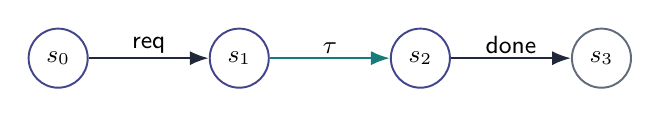
\begin{tikzpicture}[x=1cm,y=1cm]
    \node[st] (s0) at (0,0) {$s_0$}; \node[st] (s1) at (2.3,0) {$s_1$};
    \node[st] (s2) at (4.6,0) {$s_2$}; \node[terminal] (s3) at (6.9,0) {$s_3$};
    \draw[trans] (s0)--node[lab,above] {$\mathsf{req}$}(s1);
    \draw[tauedge] (s1)--node[lab,above] {$\tau$}(s2);
    \draw[trans] (s2)--node[lab,above] {$\mathsf{done}$}(s3);
  \end{tikzpicture}
  \par\vspace{2mm}
  \begin{block}{What blocking enforces}
    The $h$ and $\bar h$ actions cannot occur separately. Their joint transition is labelled $\tau$ and is not blocked.
  \end{block}
  \Takeaway{$\mathit{System}\rbb\mathit{Spec}$. Both start with $\mathsf{req}$; their derivatives are branching bisimilar.}
  \note{Let H={h,bar h}. Then s1=block_H(bar h.done.0 || h.0), s2=block_H(done.0 || 0), and s3=block_H(0 || 0). The req transitions match strictly; their derivatives are branching equivalent via the single internal handshake. Thus the systems are rooted branching equivalent and can be substituted in the extended finite contexts.}
\end{frame}

% 36 -----------------------------------------------------------------
\section{Confluence}
\begin{frame}{Confluence: different paths can be joined}
  For a binary reduction relation $\to_r$, \textbf{confluence} means
  \[
    s\step{r*}u\ \land\ s\step{r*}v
    \quad\Longrightarrow\quad
    \exists w:\ u\step{r*}w\ \land\ v\step{r*}w.
  \]
  \centering
  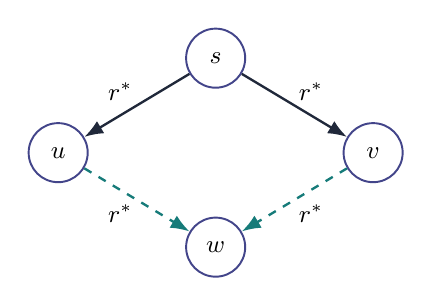
\begin{tikzpicture}[x=1cm,y=1cm]
    \node[st] (s) at (0,1.2) {$s$};
    \node[st] (u) at (-2,0) {$u$}; \node[st] (v) at (2,0) {$v$};
    \node[st] (w) at (0,-1.2) {$w$};
    \draw[trans] (s)--node[lab,above left] {$r^*$}(u);
    \draw[trans] (s)--node[lab,above right] {$r^*$}(v);
    \draw[tauedge,dashed] (u)--node[lab,below left] {$r^*$}(w);
    \draw[tauedge,dashed] (v)--node[lab,below right] {$r^*$}(w);
  \end{tikzpicture}
  \par\vspace{1mm}
  \Takeaway{For behavioural abstraction, joining internal paths is not enough: visible alternatives must also be respected.}
  \note{Only introduce the joining idea. Do not claim local confluence implies confluence without termination. The remaining slides use a local tau-focused sufficient condition from Groote and van de Pol, not the full CCS weak-confluence notion in the old slides.}
\end{frame}

% 37 -----------------------------------------------------------------
\begin{frame}{Internal confluence alone is insufficient}
  Return to
  \[
    S=\tau.a.\nil+b.\nil.
  \]
  Its $\tau$-relation is terminating and confluent: there is only one internal edge.
  \begin{columns}[T,onlytextwidth]
    \begin{column}{.43\textwidth}\centering
      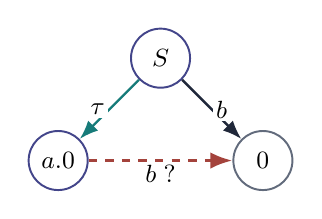
\begin{tikzpicture}[x=1cm,y=1cm]
        \node[st] (s) at (0,1.0) {$S$};
        \node[st] (a) at (-1.3,-.3) {$a.0$};
        \node[terminal] (z) at (1.3,-.3) {$0$};
        \draw[tauedge] (s)--node[lab,left] {$\tau$}(a);
        \draw[trans] (s)--node[lab,right] {$b$}(z);
        \draw[newedge,dashed] (a)--node[lab,below] {$b\;?$}(z);
      \end{tikzpicture}
    \end{column}
    \begin{column}{.54\textwidth}
      \begin{alertblock}{The missing matching behaviour}
        After the $\tau$-step, $b$ is unavailable.\\[2mm]
        Therefore $S\notbb a.\nil$.
      \end{alertblock}
    \end{column}
  \end{columns}
  \Takeaway{To prioritise an internal step, check its interaction with \emph{all competing labels}, not only $\tau$.}
\end{frame}

% 38 -----------------------------------------------------------------
\begin{frame}{A local sufficient condition: $T$-confluence}
  Choose a set $T$ of internal transitions. Write $s\step{\tau}_T t$ for an edge in $T$.
  \begin{block}{Definition}
    For every $s\step{\tau}_T t$ and $s\step{\alpha}u$, there is $v$ such that
    \[
      t\optstep{\alpha}v
      \quad\text{and}\quad
      u=v\ \text{or}\ u\step{\tau}_T v.
    \]
  \end{block}
  \begin{columns}[c,onlytextwidth]
    \begin{column}{.45\textwidth}\centering
      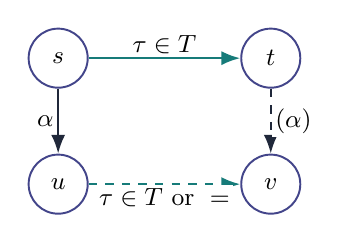
\begin{tikzpicture}[x=1cm,y=1cm]
        \node[st] (s) at (0,1.15) {$s$}; \node[st] (t) at (2.7,1.15) {$t$};
        \node[st] (u) at (0,-.45) {$u$}; \node[st] (v) at (2.7,-.45) {$v$};
        \draw[tauedge] (s)--node[lab,above] {$\tau\in T$}(t);
        \draw[trans] (s)--node[lab,left] {$\alpha$}(u);
        \draw[tauedge,dashed] (u)--node[lab,below] {$\tau\in T\ \text{or }=$}(v);
        \draw[trans,dashed] (t)--node[lab,right] {$(\alpha)$}(v);
      \end{tikzpicture}
    \end{column}
    \begin{column}{.52\textwidth}
      The right-hand step is optional only for $\alpha=\tau$.\\[2mm]
      The bottom edge, when present, must belong to the \emph{same set} $T$.
    \end{column}
  \end{columns}
  \Source{\cite[Section 2]{GP00}. This local reduction criterion is not the full CCS confluence notion.}
\end{frame}

% 39 -----------------------------------------------------------------
\begin{frame}{Confluent internal steps are inert}
  \begin{block}{Theorem}
    If the LTS is $T$-confluent, then
    \[
      s\step{\tau}_T t\quad\Longrightarrow\quad s\bb t.
    \]
    Such an internal transition is called \textbf{inert}.
  \end{block}
  \textbf{Proof idea.} Consider
  \[
    R=\Id\cup T\cup T^{-1},
  \]
  viewing $T$ as a relation on its endpoints.
  \begin{itemize}\setlength\itemsep{2mm}
    \item Match a move from $s$ using the confluence square.
    \item Match a move from $t$ by first taking $s\step{\tau}_T t$, then copying it.
  \end{itemize}
  \Takeaway{This local confluence criterion is sufficient for inertness, but not necessary.}
  \Source{\cite[Section 2]{GP00}. This inertness theorem does not require termination.}
\end{frame}

% 40 -----------------------------------------------------------------
\begin{frame}{Prioritising internal work}
  \begin{block}{A sound reduction under an explicit assumption}
    Suppose the LTS is $T$-confluent and \textbf{$\tau$-convergent}: it has no infinite $\tau$-execution. At each state with an outgoing $T$-edge, retain one such edge and remove its other outgoing transitions.
  \end{block}
  \centering
  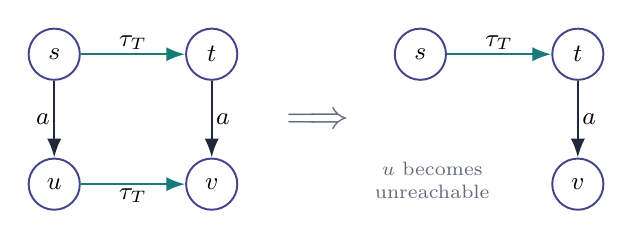
\begin{tikzpicture}[x=1cm,y=1cm,st/.append style={minimum size=6.5mm}]
    \node[st] (s) at (0,1.05) {$s$}; \node[st] (t) at (2,1.05) {$t$};
    \node[st] (u) at (0,-.6) {$u$}; \node[st] (v) at (2,-.6) {$v$};
    \draw[tauedge] (s)--node[lab,above] {$\tau_T$}(t);
    \draw[trans] (s)--node[lab,left] {$a$}(u);
    \draw[trans] (t)--node[lab,right] {$a$}(v);
    \draw[tauedge] (u)--node[lab,below] {$\tau_T$}(v);
    \node[font=\Large,text=Muted] at (3.35,.2) {$\Longrightarrow$};
    \node[st] (s2) at (4.65,1.05) {$s$}; \node[st] (t2) at (6.65,1.05) {$t$};
    \node[st] (v2) at (6.65,-.6) {$v$};
    \draw[tauedge] (s2)--node[lab,above] {$\tau_T$}(t2);
    \draw[trans] (t2)--node[lab,right] {$a$}(v2);
    \node[font=\scriptsize,text=Muted,align=center] at (4.8,-.55) {$u$ becomes\\unreachable};
  \end{tikzpicture}
  \par\vspace{1mm}
  \Takeaway{The initial states remain branching bisimilar. Removing unreachable states can shrink the graph before full minimisation.}
  \Source{\cite[Section 5]{GP00}. The guarantee is ordinary branching bisimilarity, not rooted equivalence.}
\end{frame}

% 41 -----------------------------------------------------------------
\begin{frame}{Why the convergence assumption matters}
  \centering
  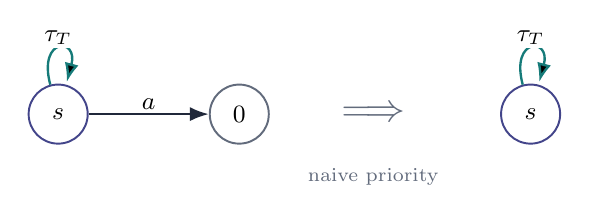
\begin{tikzpicture}[x=1cm,y=1cm]
    \node[st] (s) at (0,0) {$s$}; \node[terminal] (z) at (2.3,0) {$0$};
    \draw[tauedge] (s) edge[loop above] node[lab] {$\tau_T$} (s);
    \draw[trans] (s)--node[lab,above] {$a$}(z);
    \node[text=Muted,font=\Large] at (4,0) {$\Longrightarrow$};
    \node[st] (s2) at (6,0) {$s$};
    \draw[tauedge] (s2) edge[loop above] node[lab] {$\tau_T$} (s2);
    \node[font=\scriptsize,text=Muted] at (4,-.8) {naive priority};
  \end{tikzpicture}
  \par\vspace{4mm}
  \begin{alertblock}{The self-loop is confluent, but the reduction is wrong}
    Prioritising it removes the only $a$-transition. The resulting process is not even weakly bisimilar to the original one.
  \end{alertblock}
  \Takeaway{Inertness in the \emph{original} LTS does not justify arbitrary edge deletions. A priority policy must not trap all behaviour in an internal cycle.}
  \Source{Counterexample to unrestricted prioritisation; cf.\ \cite[Section 5]{GP00}.}
  \note{The tau-self-loop meets the local condition: a competing a-step is matched by itself, with an identity bottom edge. Thus the failure really is in prioritisation, not in confluence detection. Simply deleting tau cycles may itself erase divergence, so divergence-preserving reductions need a separate argument.}
\end{frame}

% 42 -----------------------------------------------------------------
\section{Summary}
\begin{frame}{The three requirements are distinct}
  \renewcommand{\arraystretch}{1.4}
  \begin{tabular}{@{}p{.32\textwidth}p{.62\textwidth}@{}}
    \textbf{Behavioural observations} & Traces record possible words; bisimulation also matches branching continuations.\\
    \textbf{Internal abstraction} & Weak paths abstract internal work; branching matching also preserves intermediate branching.\\
    \textbf{Infinite internal activity} & Divergence preservation prevents infinite silence from being erased.\\
    \textbf{Contextual replacement} & Rooted refinements restore congruence for choice.\\
    \textbf{State-space reduction} & Confluence gives inertness; prioritisation additionally needs convergence.
  \end{tabular}
  \vspace{2mm}
  \Takeaway{Congruence is the algebraic requirement. The observation regime determines which behavioural equivalence to use.}
  \Source{Next lecture: Mazurkiewicz traces and non-interleaving semantics; unfoldings afterwards.}
  \note{The refinements are not one linear hierarchy: rootedness and divergence preservation are incomparable and can be combined. Independence versus nondeterministic choice remains entirely for the next lecture.}
\end{frame}

\appendix
\inbackuptrue
\section{Optional material}

% A1 ----------------------------------------------------------------
\begin{frame}{\optional The weak bisimulation game}
  A position is a pair of states $(p,q)$.
  \begin{enumerate}\setlength\itemsep{2.5mm}
    \item Spoiler chooses either side and one transition, say $p\step{\alpha}p'$.
    \item Duplicator chooses a \emph{finite} matching path $q\wstep{\alpha}q'$.
    \item Continue from $(p',q')$.
  \end{enumerate}
  \begin{block}{Winning condition}
    Spoiler wins when a chosen transition has no matching response.\\
    Duplicator wins infinite plays, and positions where Spoiler has no move.
  \end{block}
  \Takeaway{$p\wb q$ exactly when Duplicator has a winning strategy from $(p,q)$.}
  \begin{exampleblock}{A silent commitment gives Spoiler a strategy}
    For $P=\tau.(a.\nil+b.\nil)$ and $Q=\tau.a.\nil+\tau.b.\nil$, start with $Q\step{\tau}a.\nil$. Either response from $P$ still permits $b$.
  \end{exampleblock}
  \note{Choose Q and its tau-transition to a.0. After either response from P, choose the weakly available b as a short sequence of challenges. If Duplicator stayed at P, Spoiler first takes its tau, then b.}
\end{frame}

% A2 ----------------------------------------------------------------
\begin{frame}{\optional Invisible does not mean irrelevant}
  \[
    P=\tau.(a.\nil+b.\nil),\qquad
    Q=\tau.a.\nil+\tau.b.\nil.
  \]
  \begin{columns}[T,onlytextwidth]
    \begin{column}{.49\textwidth}\centering
      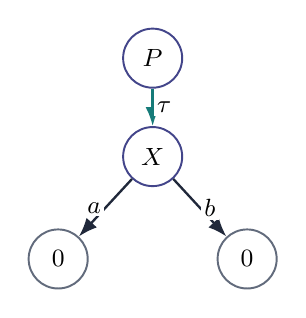
\begin{tikzpicture}[x=1cm,y=1cm]
        \node[st] (p) at (0,1.25) {$P$};
        \node[st] (x) at (0,0) {$X$};
        \node[terminal] (z1) at (-1.2,-1.3) {$0$};
        \node[terminal] (z2) at (1.2,-1.3) {$0$};
        \draw[tauedge] (p)--node[lab,right] {$\tau$}(x);
        \draw[trans] (x)--node[lab,left] {$a$}(z1);
        \draw[trans] (x)--node[lab,right] {$b$}(z2);
      \end{tikzpicture}
    \end{column}
    \begin{column}{.49\textwidth}\centering
      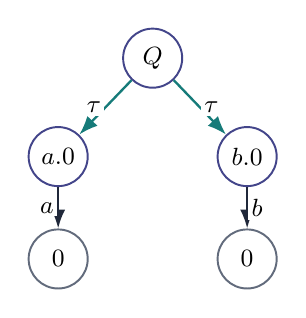
\begin{tikzpicture}[x=1cm,y=1cm]
        \node[st] (q) at (0,1.25) {$Q$};
        \node[st] (u) at (-1.2,0) {$a.0$};
        \node[st] (v) at (1.2,0) {$b.0$};
        \node[terminal] (z1) at (-1.2,-1.3) {$0$};
        \node[terminal] (z2) at (1.2,-1.3) {$0$};
        \draw[tauedge] (q)--node[lab,left] {$\tau$}(u);
        \draw[tauedge] (q)--node[lab,right] {$\tau$}(v);
        \draw[trans] (u)--node[lab,left] {$a$}(z1);
        \draw[trans] (v)--node[lab,right] {$b$}(z2);
      \end{tikzpicture}
    \end{column}
  \end{columns}
  \uncover<2->{\Takeaway{$P\notwb Q$: after $Q\step{\tau}a.0$, every possible silent response of $P$ still allows $b$.}}
  \note{Both P and X can perform b weakly. Neither can be related by a weak bisimulation to a.0. This also explains why the weak-bisimulation transfer clause must cover tau, not only visible labels.}
\end{frame}

% A3 ----------------------------------------------------------------
\begin{frame}{\optional Weak bisimilarity by saturation}
  \begin{block}{Saturated LTS}
    Keep the states and add an edge for every weak transition:
    \[
      p\step{\alpha}_{\mathrm{sat}}q
      \quad\Longleftrightarrow\quad
      p\wstep{\alpha}q
      \qquad(\alpha\in\Act).
    \]
    This includes \emph{all} $\tau^*$-shortcuts, not just $\tau$-self-loops.
  \end{block}
  \begin{block}{Characterisation}
    \[
      p\wb q\text{ in }T
      \quad\Longleftrightarrow\quad
      p\sim q\text{ in }T_{\mathrm{sat}}.
    \]
  \end{block}
  \Takeaway{Compute $\tau$-reachability, build the saturated graph, then reuse strong-bisimulation partition refinement.}
  \Source{Adapted and made explicit from the saturation idea in the supplied weak-bisimulation slides.}
\end{frame}

% A4 ----------------------------------------------------------------
\begin{frame}{\optional Why saturation works, and what it costs}
  \textbf{From weak to strong.} Repeatedly apply the weak transfer condition along the finite path
  \[
    \tau^*\,a\,\tau^*\quad\text{or}\quad\tau^*.
  \]
  Concatenating the responses gives a matching saturated edge with a related endpoint.
  \vspace{3mm}
  \textbf{From strong to weak.} Every original edge is a saturated edge; a matching saturated edge is exactly an allowed weak response.
  \begin{alertblock}{Finite-state cost}
    With $n$ states and $k=|\Act|$ labels, the saturated LTS can have up to $kn^2$ edges. The reduction can destroy sparsity. Include the cost of constructing saturation, not only of minimising it.
  \end{alertblock}
  \Source{This also proves that weak bisimilarity is an equivalence relation.}
\end{frame}

% A5 ----------------------------------------------------------------
\begin{frame}{\optional The precise divergence-preservation clause}
  Let $R$ be a symmetric branching bisimulation.
  \begin{block}{Explicit divergence condition}
    If $p\,R\,q$ and there is an infinite path
    \[
      p=p_0\step{\tau}p_1\step{\tau}p_2\cdots
      \quad\text{with }p_i\,R\,q\text{ for every }i,
    \]
    then there must be an infinite path
    \[
      q=q_0\step{\tau}q_1\step{\tau}q_2\cdots
      \quad\text{with }p_i\,R\,q_j\text{ for all }i,j.
    \]
  \end{block}
  We write $p\dbb q$ if some branching bisimulation satisfying this condition relates them.
  \Takeaway{The condition concerns divergence \emph{within related behaviour}; it is not merely an extra Boolean label saying ``can diverge''.}
  \Source{\cite[Section 3]{GLT09}; also \cite[Definition 2.1]{GLS20}.}
\end{frame}

% A6 ----------------------------------------------------------------
\begin{frame}{\optional The inertness proof in detail}
  Let $s\step{\tau}_T t$ and put $R=\Id\cup T\cup T^{-1}$.
  \par\vspace{2mm}
  \textbf{A move from $s$.} For $s\step{\alpha}u$, confluence gives
  \[
    t\optstep{\alpha}v,\qquad u=v\text{ or }u\step{\tau}_T v.
  \]
  The source pair is $(s,t)\in R$ and the target pair is $(u,v)\in R$.
  \par\vspace{2mm}
  \textbf{A move from $t$.} For $t\step{\alpha}v$, respond with
  \[
    s\step{\tau}_T t\step{\alpha}v.
  \]
  Use the identity pairs $(t,t)$ before the matching action and $(v,v)$ afterwards.
  \Takeaway{Identity and converse pairs give the remaining cases. Thus $R$ is a branching bisimulation.}
  \Source{Proof for the sufficient condition in \cite{GP00}.}
\end{frame}

% A7 ----------------------------------------------------------------
\begin{frame}{\optional Weak modal observations}
  Replace the one-step modality of Hennessy--Milner logic by a weak modality:
  \[
    \varphi::=\top\mid\neg\varphi\mid\varphi\land\varphi
       \mid\langle\!\langle\alpha\rangle\!\rangle\varphi,
       \qquad \alpha\in\Act,
  \]
  \[
    p\models\langle\!\langle\alpha\rangle\!\rangle\varphi
    \quad\Longleftrightarrow\quad
    \exists q:\ p\wstep{\alpha}q\ \land\ q\models\varphi.
  \]
  \begin{block}{Finite LTSs}
    Two states are weakly bisimilar iff they satisfy the same formulas of this logic.
  \end{block}
  \textbf{Reason:} apply the Hennessy--Milner theorem to the saturated LTS.
  \begin{alertblock}{Keep the $\tau$-modality}
    $a.\nil+\tau.\nil$ satisfies
    $\langle\!\langle\tau\rangle\!\rangle\neg\langle\!\langle a\rangle\!\rangle\top$,
    but $a.\nil$ does not.
  \end{alertblock}
  \note{This is an explicit deduction from saturation and the finite-state HML theorem from Lecture 3. It makes no unqualified claim about CTL preservation on arbitrary action-labelled LTSs.}
\end{frame}

\section{References}
% A8 ----------------------------------------------------------------
\begin{frame}{References: abstraction and congruence}
  \small
  \begin{thebibliography}{GLS20}
    \bibitem[GW96]{GW96}
      R. J. van Glabbeek and W. P. Weijland.
      \emph{Branching Time and Abstraction in Bisimulation Semantics}.
      Journal of the ACM 43(3), 555--600, 1996.
      \newblock\href{https://theory.stanford.edu/~rvg/abstraction/}{Author-hosted version}.
    \bibitem[GLT09]{GLT09}
      R. J. van Glabbeek, B. Luttik, and N. Tr\v{c}ka.
      \emph{Branching Bisimilarity with Explicit Divergence}.
      Fundamenta Informaticae 93(4), 371--392, 2009.
      \newblock\href{https://arxiv.org/abs/0812.3068}{arXiv:0812.3068}.
    \bibitem[GLS20]{GLS20}
      R. J. van Glabbeek, B. Luttik, and L. Spaninks.
      \emph{Rooted Divergence-Preserving Branching Bisimilarity is a Congruence}.
      Logical Methods in Computer Science 16(3:14), 2020.
      \newblock\href{https://arxiv.org/abs/1801.01180}{arXiv:1801.01180}.
  \end{thebibliography}
\end{frame}

% A9 ----------------------------------------------------------------
\begin{frame}{References: reduction and source material}
  \small
  \begin{thebibliography}{MCS}
    \bibitem[GP00]{GP00}
      J. F. Groote and J. van de Pol.
      \emph{State Space Reduction using Partial $\tau$-Confluence}.
      CWI report SEN-R0008, 2000, especially Sections 2 and 5.
      \newblock\href{https://ir.cwi.nl/pub/4446}{CWI repository record}.
    \bibitem[MCS]{MCS}
      R. J. van Glabbeek.
      \emph{Modelling Concurrent Systems: course notes}.
      University of Edinburgh, 2024, especially Lectures 6--8.
      \newblock\href{https://homepages.inf.ed.ac.uk/rvangla/MCS/notes.html}{Author's course notes}.
  \end{thebibliography}
  \begin{block}{Basis and additions}
    The supplied weak-bisimulation and process-algebra slides provide the starting material. Branching bisimulation, divergence, and rootedness are developed for this lecture. The former global CCS-confluence section is replaced by the local $\tau$-reduction criterion above.
  \end{block}
  \Source{A source map, corrections to the old slides, and teaching cautions are recorded in \texttt{lecture5\_notes.md}.}
\end{frame}

\end{document}
'
% Sources, scope changes, and technical cautions: lecture5_notes.md.
\ifdefined\HANDOUT
  \documentclass[handout,aspectratio=169,11pt]{beamer}
\else
  \documentclass[aspectratio=169,11pt]{beamer}
\fi
\usepackage[T1]{fontenc}
\usepackage[utf8]{inputenc}
\usepackage{lmodern}
\usepackage{amsmath,amssymb,mathtools,booktabs,array}
\usepackage{tikz}
\usetikzlibrary{arrows.meta,positioning,calc,fit,backgrounds}
\usepackage{appendixnumberbeamer}
\usefonttheme{professionalfonts}

\definecolor{Ink}{HTML}{20283A}
\definecolor{Indigo}{HTML}{43458A}
\definecolor{Pale}{HTML}{F0F0F8}
\definecolor{Teal}{HTML}{167B79}
\definecolor{PaleTeal}{HTML}{EAF5F3}
\definecolor{Warn}{HTML}{A4433C}
\definecolor{PaleWarn}{HTML}{FBF0EE}
\definecolor{Muted}{HTML}{626B7C}
\setbeamercolor{normal text}{fg=Ink,bg=white}
\setbeamercolor{structure}{fg=Indigo}
\setbeamercolor{frametitle}{fg=Indigo}
\setbeamercolor{title}{fg=Indigo}
\setbeamercolor{block title}{fg=Indigo,bg=Pale}
\setbeamercolor{block body}{fg=Ink,bg=Pale}
\setbeamercolor{block title example}{fg=Teal,bg=PaleTeal}
\setbeamercolor{block body example}{fg=Ink,bg=PaleTeal}
\setbeamercolor{block title alerted}{fg=Warn,bg=PaleWarn}
\setbeamercolor{block body alerted}{fg=Ink,bg=PaleWarn}
\setbeamertemplate{blocks}[rounded][shadow=false]
\setbeamertemplate{navigation symbols}{}
\setbeamertemplate{bibliography item}[text]
\pdfstringdefDisableCommands{\def\translate#1{#1}}
\setbeamersize{text margin left=8mm,text margin right=8mm}
\setbeamerfont{frametitle}{size=\Large,series=\bfseries}
\setbeamerfont{block title}{size=\normalsize,series=\bfseries}
\setbeamerfont{footnote}{size=\scriptsize}
\setbeamertemplate{itemize item}{\small\raise0.2ex\hbox{\textbullet}}
\setbeamertemplate{itemize subitem}{\tiny\raise0.2ex\hbox{\textbullet}}
\setbeamercovered{invisible}
\setbeameroption{hide notes}
\newif\ifinbackup
\inbackupfalse
\setbeamertemplate{headline}{\color{Indigo}\rule{\paperwidth}{0.5mm}}
\setbeamertemplate{footline}{%
  \leavevmode\hbox{%
    \begin{beamercolorbox}[wd=.79\paperwidth,ht=3.5mm,dp=2mm,leftskip=8mm]{normal text}%
      \color{Muted}\scriptsize Theory of Concurrency\enspace/\enspace Lecture 5\enspace/\enspace\insertsectionhead
    \end{beamercolorbox}%
    \begin{beamercolorbox}[wd=.21\paperwidth,ht=3.5mm,dp=2mm,rightskip=8mm plus1fil]{normal text}%
      \hfill\color{Muted}\scriptsize\ifinbackup Backup\enspace\fi\insertframenumber\,/\,\inserttotalframenumber
    \end{beamercolorbox}%
  }}
\setlength{\abovedisplayskip}{6pt}
\setlength{\belowdisplayskip}{6pt}
\newcommand{\step}[1]{\xrightarrow{#1}}
\newcommand{\wstep}[1]{\xRightarrow{#1}}
\newcommand{\silent}{\mathrel{\Rightarrow}}
\newcommand{\optstep}[1]{\xrightarrow{(#1)}}
\newcommand{\wb}{\mathrel{\approx_{\mathrm w}}}
\newcommand{\bb}{\mathrel{\approx_{\mathrm b}}}
\newcommand{\rbb}{\mathrel{\approx_{\mathrm{rb}}}}
\newcommand{\rwb}{\mathrel{\approx_{\mathrm{rw}}}}
\newcommand{\dbb}{\mathrel{\approx_{\mathrm b}^{\Delta}}}
\newcommand{\notwb}{\mathrel{\not\approx_{\mathrm w}}}
\newcommand{\notbb}{\mathrel{\not\approx_{\mathrm b}}}
\newcommand{\notrbb}{\mathrel{\not\approx_{\mathrm{rb}}}}
\newcommand{\notdbb}{\mathrel{\not\approx_{\mathrm b}^{\Delta}}}
\newcommand{\nil}{\mathbf 0}
\newcommand{\Act}{\Sigma_\tau}
\newcommand{\blockact}[2]{\operatorname{block}_{#1}(#2)}
\newcommand{\hide}[2]{\operatorname{hide}_{#1}(#2)}
\newcommand{\restr}[2]{(\nu #1)\,#2}
\newcommand{\Tr}{\operatorname{Tr}}
\newcommand{\CT}{\operatorname{CT}}
\newcommand{\Id}{\operatorname{Id}}
\newcommand{\Source}[1]{\par\vspace{2mm}{\scriptsize\color{Muted}#1\par}}
\newcommand{\Takeaway}[1]{\begin{exampleblock}{}#1\end{exampleblock}}
\newcommand{\optional}{\textcolor{Muted}{\scriptsize OPTIONAL}\quad}
\tikzset{
  >=Latex,
  st/.style={circle,draw=Indigo,line width=.7pt,fill=white,minimum size=7.5mm,inner sep=1pt,font=\small},
  terminal/.style={st,draw=Muted},
  trans/.style={->,line width=.85pt,draw=Ink},
  tauedge/.style={trans,draw=Teal},
  newedge/.style={trans,draw=Warn,line width=1.1pt},
  rel/.style={dashed,draw=Teal,line width=.85pt},
  lab/.style={font=\small,fill=white,inner sep=1.2pt},
  tinylabel/.style={font=\scriptsize,fill=white,inner sep=1pt},
  panel/.style={rounded corners=2mm,fill=Pale,draw=none,inner sep=4mm}
}
\title{Congruence and abstraction}
\subtitle{Lecture 5: Weak and branching bisimulation}
\author{Piotr Hofman}
\institute{Theory of Concurrency}
\date{}

\begin{document}

% 1 -----------------------------------------------------------------
\section{Overview}
\begin{frame}[plain]
  \vspace{8mm}
  {\color{Muted}\large THEORY OF CONCURRENCY\par}
  \vspace{6mm}
  {\color{Indigo}\LARGE\bfseries Congruence and abstraction\par}
  \vspace{3mm}
  {\Large From strong to weak and branching bisimulation\par}
  \vspace{7mm}
  {\large Lecture 5\quad\textcolor{Muted}{Piotr Hofman}\par}
  \vfill
  \begin{beamercolorbox}[sep=3mm,wd=\textwidth]{block body}
    First: when does equivalence support substitution?\\[1mm]
    Then: how much internal behaviour may an abstraction forget?
  \end{beamercolorbox}
  \vspace{3mm}
\end{frame}

% 2 -----------------------------------------------------------------


% 3 -----------------------------------------------------------------
\section{Congruence}
\begin{frame}{Congruence: equality compatible with operations}
  Let $\mathcal A$ be a set equipped with operations $f:\mathcal A^n\to\mathcal A$.
  \begin{block}{Definition}
    An equivalence relation $\equiv$ is a \textbf{congruence} if, for every operation $f$,
    \[
      x_i\equiv y_i\ (1\leq i\leq n)
      \quad\Longrightarrow\quad
      f(x_1,\ldots,x_n)\equiv f(y_1,\ldots,y_n).
    \]
  \end{block}
  \begin{exampleblock}{A familiar example: integers modulo $2$}
    If $x\equiv_2 x'$ and $y\equiv_2 y'$, then
    \[
      x+y\equiv_2 x'+y',\qquad xy\equiv_2 x'y'.
    \]
    Parity is a congruence for addition and multiplication.
  \end{exampleblock}
  \Takeaway{The requirement depends on the chosen operations, not only on the equivalence relation.}
  \Source{The general algebraic definition; process congruence is its application to system constructors.}
\end{frame}

% 4 -----------------------------------------------------------------
\begin{frame}{Why congruence gives a well-defined quotient}
  Every equivalence partitions $\mathcal A$ into classes $[x]$.
  We would like to define operations on classes by
  \[
    \overline f([x_1],\ldots,[x_n])=[f(x_1,\ldots,x_n)].
  \]
  \begin{block}{The role of congruence}
    The result must not depend on the representatives $x_1,\ldots,x_n$.
    This is \emph{exactly} the compatibility requirement in the definition.
  \end{block}
  \begin{exampleblock}{For systems}
    Build a larger system from the behavioural classes of its components,
    without inspecting which representatives were chosen.
  \end{exampleblock}
  \Takeaway{Congruence makes ``compute with behaviours instead of implementations'' mathematically meaningful.}
  \note{This is a quotient algebra of processes under constructors. It is distinct from the quotient of states inside a single LTS used for partition-refinement minimisation. Do not infer that an arbitrary state equivalence yields a behaviour-preserving quotient transition system.}
\end{frame}

% 5 -----------------------------------------------------------------
\section{Processes and contexts}
\begin{frame}{Processes and a small collection of operations}
  \begin{block}{For now: every action is visible}
    An LTS is $T=(S,\Sigma,\to)$, with ${\to}\subseteq S\times\Sigma\times S$.
    A process is an LTS with a distinguished state.
  \end{block}
  \renewcommand{\arraystretch}{1.4}
  \begin{tabular}{@{}p{.21\textwidth}p{.74\textwidth}@{}}
    $\nil$ & No outgoing transitions.\\
    $a.P$ & Perform $a\in\Sigma$, then behave as $P$.\\
    $P+Q$ & Perform a first transition of one summand; discard the other.\\
    $\blockact{H}{P}$ & Disable transitions labelled in $H\subseteq\Sigma$.
  \end{tabular}
  \vspace{2mm}
  \Takeaway{These are operations on LTSs; expressions are just convenient notation.}
  \Source{No acceptance predicate or successful-termination marker. Cyclic processes may be given directly as graphs.}
  \note{The initial fragment deliberately needs neither internal actions nor a full process calculus. Action blocking is written explicitly instead of using a channel-restriction shorthand. Later we add hiding and CCS parallel composition.}
\end{frame}




% 6 -----------------------------------------------------------------
\begin{frame}{The operations are defined by transition rules}
  \begin{block}{Prefix and choice}
    \[
      \frac{}{a.P\step{a}P}
      \qquad
      \frac{P\step{a}P'}{P+Q\step{a}P'}
      \qquad
      \frac{Q\step{a}Q'}{P+Q\step{a}Q'}.
    \]
  \end{block}
  \begin{block}{Blocking: restriction to allowed actions}
    \[
      \frac{P\step{a}P'}{\blockact{H}{P}\step{a}\blockact{H}{P'}}
      \qquad a\notin H.
    \]
    No rule permits an action in $H$.
  \end{block}
  \[
    a.b.\nil+a.c.\nil\step{a}b.\nil,
    \qquad \blockact{\{c\}}{c.\nil}\sim\nil.
  \]
  \Source{Prefix and choice follow the supplied CCS rules; blocking is the label-based restriction operation.}
\end{frame}

% 7 -----------------------------------------------------------------
\begin{frame}{Process congruence: replacement in every context}
  A finite \textbf{one-hole context} is built from the chosen operations:
  \[
    C[-]::=[-]\mid a.C[-]\mid C[-]+R\mid R+C[-]\mid\blockact{H}{C[-]}.
  \]
  Here $R$ is any fixed process. $C[P]$ is obtained by filling the hole with $P$.
  \begin{block}{Equivalent formulation of compatibility}
    \[
      P\equiv Q\quad\Longrightarrow\quad C[P]\equiv C[Q]
      \quad\text{for every allowed }C[-].
    \]
  \end{block}
  \begin{alertblock}{A different requirement from logical preservation}
    Satisfying the same formulas concerns \emph{observations}. Congruence concerns
    \emph{operations that build larger systems}.
  \end{alertblock}
  \Source{Adapted from the supplied context definitions; see also \cite{MCS}.}
  \note{Operator compatibility implies context compatibility by induction on the finite context. The converse follows by fixing all but one argument of an operation and replacing the arguments one at a time. No recursion-binding contexts are included.}
\end{frame}


\begin{frame}{Congruence: from basic operations to contexts}
  \begin{block}{Lemma}
    Let $\equiv$ be an equivalence relation on processes.
    The following conditions are equivalent:
    \begin{enumerate}
      \item $\equiv$ is compatible with every basic process operation.
      \item For every finite one-hole context $C[-]$ built from these
            operations and fixed processes,
            \[
              P\equiv Q \quad\Longrightarrow\quad C[P]\equiv C[Q].
            \]
    \end{enumerate}
  \end{block}

  \begin{block}{Proof sketch}
    \textbf{$(1)\Rightarrow(2)$.}
    Structural induction on $C[-]$: apply compatibility at each
    constructor and reflexivity for the fixed arguments.

    \medskip
    \textbf{$(2)\Rightarrow(1)$.}
    Fix all arguments of a basic operation except one.
    This gives a one-hole context, hence compatibility in that argument.
    Replace the arguments one at a time and use transitivity.
  \end{block}

 % \Takeaway{Compatibility with contexts is not an additional requirement: checking the basic operations suffices.}
\end{frame}

% 8 -----------------------------------------------------------------
\begin{frame}{Strong bisimilarity is a congruence}
  \begin{block}{Theorem for the operators just defined}
    \[
      P\sim Q\quad\Longrightarrow\quad C[P]\sim C[Q].
    \]
  \end{block}
  \textbf{Example: preservation by choice.} Assume $P\sim Q$ and fix $R$.
  \begin{itemize}\setlength\itemsep{3mm}
    \item A move of $P+R$ coming from $P$ is matched by a move of $Q$ with a bisimilar successor.
    \item A move coming from $R$ is matched by the identical move of $R$.
  \end{itemize}
  The same reasoning applies in the reverse direction.
  %\Takeaway{Prove compatibility with each constructor, then use induction on the context.}
  \Source{Compatibility for the displayed constructors; see \cite{MCS}.}
  \note{Explicit correction to old prezentacja(1).pdf, page 33: the printed claim 'not a congruence' contradicts its proof sketch and is false for these operators. At this point only prefix, choice and blocking are in scope. Prefix gives related successors; blocking filters the same labels on both sides. Compatibility with parallel and hiding will be used after those operations have been introduced.}
\end{frame}

% 9 -----------------------------------------------------------------
\section{Traces versus bisimulation}
\begin{frame}{Trace equivalence is also a congruence}
  Use the language of \textbf{all finite traces}, including the empty word:
  \[
    \Tr(P)=\{w\in\Sigma^*: P\step{w}P'\text{ for some }P'\}.
  \]
  \begin{block}{The trace language of a composite is determined by its operands}
    \[
    \begin{aligned}
      \Tr(\nil)&=\{\varepsilon\},\\
      \Tr(a.P)&=\{\varepsilon\}\cup a\Tr(P),\\
      \Tr(P+Q)&=\Tr(P)\cup\Tr(Q),\\
      \Tr(\blockact{H}{P})&=\Tr(P)\cap(\Sigma\setminus H)^*.
    \end{aligned}
    \]
  \end{block}
  \Takeaway{Congruence \emph{alone} does not justify choosing bisimulation over trace equivalence. We also need to specify what must be observed.}
  \note{This is the all-finite-traces convention, not an accepted language 
  with designated final states and not the 
  infinite-word semantics of LTL. Standard CCS 
  finite visible trace equivalence is also compositional, 
  but its extra operators are not needed for the argument here.}
\end{frame}




% 10 -----------------------------------------------------------------
\begin{frame}{The same traces, different choices after interaction}
  \[
    P=a.(b.\nil+c.\nil),\qquad Q=a.b.\nil+a.c.\nil.
  \]
  \begin{columns}[T,onlytextwidth]
    \begin{column}{.48\textwidth}\centering
      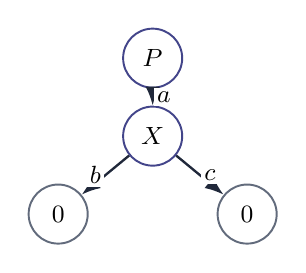
\begin{tikzpicture}[x=1cm,y=.9cm]
        \node[st] (p) at (0,1.1) {$P$}; \node[st] (x) at (0,0) {$X$};
        \node[terminal] (z1) at (-1.2,-1.1) {$0$}; \node[terminal] (z2) at (1.2,-1.1) {$0$};
        \draw[trans] (p)--node[lab,right] {$a$}(x);
        \draw[trans] (x)--node[lab,left] {$b$}(z1);
        \draw[trans] (x)--node[lab,right] {$c$}(z2);
      \end{tikzpicture}
    \end{column}
    \begin{column}{.48\textwidth}\centering
      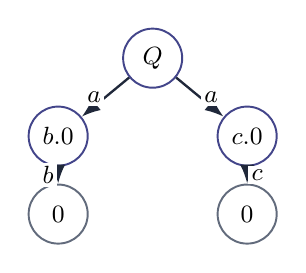
\begin{tikzpicture}[x=1cm,y=.9cm]
        \node[st] (q) at (0,1.1) {$Q$};
        \node[st] (u) at (-1.2,0) {$b.0$}; \node[st] (v) at (1.2,0) {$c.0$};
        \node[terminal] (z1) at (-1.2,-1.1) {$0$}; \node[terminal] (z2) at (1.2,-1.1) {$0$};
        \draw[trans] (q)--node[lab,left] {$a$}(u); \draw[trans] (q)--node[lab,right] {$a$}(v);
        \draw[trans] (u)--node[lab,left] {$b$}(z1); \draw[trans] (v)--node[lab,right] {$c$}(z2);
      \end{tikzpicture}
    \end{column}
  \end{columns}
  \[
    \Tr(P)=\Tr(Q)=\{\varepsilon,a,ab,ac\},\qquad P\not\sim Q.
  \]
  \Takeaway{$P$ satisfies $\langle a\rangle(\langle b\rangle\top\land\langle c\rangle\top)$; $Q$ does not.}
\end{frame}




% 11 -----------------------------------------------------------------
\begin{frame}{Deadlock observations can destroy congruence}
  A \textbf{finite completed trace} ends in a deadlock:
  \[
    \CT(P)=\{w:P\step{w}P'\text{ and }P'\text{ has no outgoing transition}\}.
  \]
  For the preceding $P$ and $Q$, $\CT(P)=\CT(Q)=\{ab,ac\}$.
  \begin{alertblock}{An environment that blocks $c$}
    \[
    \begin{aligned}
      \CT(\blockact{\{c\}}{P})&=\{ab\},\\
      \CT(\blockact{\{c\}}{Q})&=\{a,ab\}.
    \end{aligned}
    \]
    The second process can commit to its $c$-branch and become stuck after $a$.
  \end{alertblock}
  \Takeaway{The ordinary trace languages still agree. Completed-trace equality is not a congruence for blocking.}
  \note{For general infinite-state systems, completed-trace equivalence is often defined to preserve both all traces and completed traces. This example refutes congruence under either convention: the original pair agrees on both. All displayed processes are finite and have no successful-termination predicate.}
\end{frame}

% 12 -----------------------------------------------------------------
\begin{frame}{Why make bisimulation our baseline?}
  \begin{block}{The verification objective}
    Preserve the available continuations after every matched interaction,
    including branching observations and deadlock behaviour.
  \end{block}
  \renewcommand{\arraystretch}{1.45}
  \begin{tabular}{@{}p{.26\textwidth}p{.68\textwidth}@{}}
    \textbf{Logical} & Strong bisimulation preserves HML; on Kripke structures, its label-preserving version preserves CTL$^*$.\\
    \textbf{Algebraic} & It supports substitution under the chosen constructors.\\
    \textbf{Proof-theoretic} & A witness is checked locally by matching transitions; finite-state minimisation uses partition refinement.
  \end{tabular}
  \vspace{2mm}
  \note{Do not say that traces cannot express liveness: 
  equality of infinite state-labelled trace languages preserves LTL, 
  including LTL liveness. 
  Nor do deadlock and compositionality alone uniquely characterise bisimulation: 
  failure/testing semantics offers intermediate alternatives. 
  The chosen baseline reflects this course's branching-time analysis and local proof methods.}
\end{frame}

% 13 -----------------------------------------------------------------
\section{Internal actions and abstraction}
\begin{frame}{Now add internal actions and abstraction}
  Let $\Act=\Sigma\cup\{\tau\}$, with $\tau\notin\Sigma$.\\[1mm]
  $a,b,c\in\Sigma$ are visible; $\alpha\in\Act$ may be internal.\par\vspace{2mm}
  \centering
  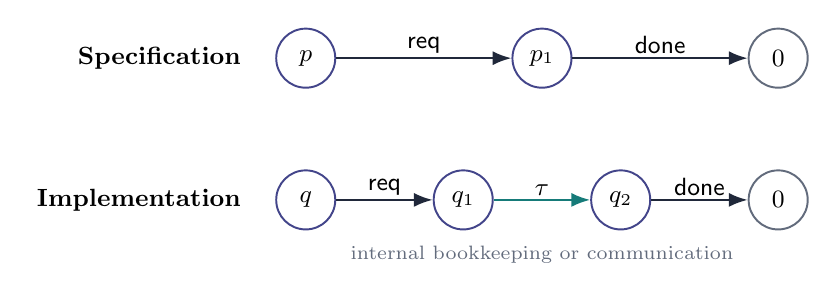
\begin{tikzpicture}[x=1cm,y=1cm]
    \node[anchor=east,font=\small\bfseries] at (-.7,1.35) {Specification};
    \node[st] (p) at (0,1.35) {$p$};
    \node[st] (p1) at (3,1.35) {$p_1$};
    \node[terminal] (p2) at (6,1.35) {$0$};
    \draw[trans] (p)--node[lab,above] {$\mathsf{req}$}(p1);
    \draw[trans] (p1)--node[lab,above] {$\mathsf{done}$}(p2);
    \node[anchor=east,font=\small\bfseries] at (-.7,-.45) {Implementation};
    \node[st] (q) at (0,-.45) {$q$};
    \node[st] (q1) at (2,-.45) {$q_1$};
    \node[st] (q2) at (4,-.45) {$q_2$};
    \node[terminal] (q3) at (6,-.45) {$0$};
    \draw[trans] (q)--node[lab,above] {$\mathsf{req}$}(q1);
    \draw[tauedge] (q1)--node[lab,above] {$\tau$}(q2);
    \draw[trans] (q2)--node[lab,above] {$\mathsf{done}$}(q3);
    \node[font=\scriptsize,text=Muted] at (3,-1.15) {internal bookkeeping or communication};
  \end{tikzpicture}
  \par\vspace{2mm}
  \begin{block}{External behaviour}
    Strong bisimulation distinguishes the initial states because of the internal step.
    We seek a coarser relation that can abstract from this bookkeeping.
  \end{block}
  \note{Spoiler performs req and then the implementation's tau. The specification cannot match that tau strongly. Do not identify hiding with edge deletion: hiding changes labels, retaining the intermediate states and alternatives.}
\end{frame}

% 14 -----------------------------------------------------------------
\begin{frame}{The simplified process algebra with internal actions}
  Let $\Sigma$ contain the visible actions, with $\tau\notin\Sigma$.
  Write
  \[
    \Sigma_\tau=\Sigma\cup\{\tau\},
    \qquad \alpha\in\Sigma_\tau,
    \qquad H\subseteq\Sigma.
  \]

  \begin{block}{Process constructors}
    \renewcommand{\arraystretch}{1.4}
    \begin{tabular}{@{}p{.25\textwidth}p{.69\textwidth}@{}}
      $\nil$
        & No outgoing transitions, not even internal ones.\\
      $\alpha.P$
        & Perform $\alpha$, then behave as $P$.
          In particular, $\tau.P\step{\tau}P$.\\
      $P+Q$
        & The first transition of either summand selects that
          summand and discards the other, even if its label is $\tau$.\\
      $\blockact{H}{P}$
        & Remove transitions labelled in $H$.
          Other transitions, including $\tau$-transitions, remain.\\
      $\hide{H}{P}$ \alert{(new)}
        & Replace labels in $H$ by $\tau$.
          Retain all states and transitions; leave other labels unchanged.


        \end{tabular}
  \end{block}


\end{frame}


\begin{frame}{The simplified process algebra with internal actions}
  Let $\Sigma$ contain the visible actions, with $\tau\notin\Sigma$.
  Write
  \[
    \Sigma_\tau=\Sigma\cup\{\tau\},
    \qquad \alpha\in\Sigma_\tau,
    \qquad H\subseteq\Sigma.
  \]


  \begin{exampleblock}{Blocking prevents an action; hiding conceals it}
    \[
      \blockact{\{a\}}{a.b.\nil}\sim\nil,
      \qquad
      \hide{\{a\}}{a.b.\nil}\sim\tau.b.\nil.
    \]
    After hiding $a$, the process can still reach and perform $b$.
  \end{exampleblock}
\end{frame}



\begin{frame}{Operational rules: an internal step is still a step}
  Throughout, $\alpha\in\Sigma_\tau$ and $H\subseteq\Sigma$.
  The process $\nil$ has no transition rules.

  \begin{block}{Prefix and choice: the same rules for visible and internal actions}
    \[
      \frac{}{\alpha.P\step{\alpha}P}
      \qquad
      \frac{P\step{\alpha}P'}{P+Q\step{\alpha}P'}
      \qquad
      \frac{Q\step{\alpha}Q'}{P+Q\step{\alpha}Q'}.
    \]
  \end{block}

  \begin{block}{Blocking and hiding}
    \[
      \frac{P\step{\alpha}P'}
           {\blockact{H}{P}\step{\alpha}\blockact{H}{P'}}
      \;(\alpha\notin H)
      \qquad
      \frac{P\step{\alpha}P'}
           {\hide{H}{P}\step{h_H(\alpha)}\hide{H}{P'}},
    \]
    where
    \[
      h_H(\alpha)=
      \begin{cases}
        \tau,   & \alpha\in H,\\
        \alpha, & \alpha\notin H.
      \end{cases}
      \qquad\text{In particular, }h_H(\tau)=\tau.
    \]
  \end{block}

\end{frame}



\begin{frame}{Operational rules: an internal step is still a step}
 

  \begin{alertblock}{A silent transition can resolve a choice}
    \[
      \tau.a.\nil+b.\nil\step{\tau}a.\nil,
      \qquad
      \tau.a.\nil+b.\nil\step{b}\nil.
    \]
    Both initial transitions are possible: $\tau$ has no priority.
    If the $\tau$-step occurs, the successor is $a.\nil$,
    \textbf{not} $a.\nil+b.\nil$: the $b$-alternative disappears.
  \end{alertblock}
\end{frame}

% 15 -----------------------------------------------------------------
\begin{frame}{A tempting but inadequate proposal: ignore silent moves}
  Suppose we compare only visible behaviour, allowing internal work before and after it,
  but impose \emph{no obligation} on a purely internal move.
  \[
    P=a.\nil+\tau.\nil,\qquad Q=a.\nil.
  \]
  \centering
  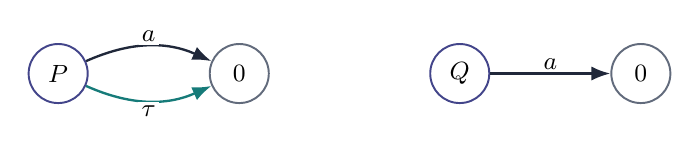
\begin{tikzpicture}[x=1cm,y=1cm]
    \node[st] (p) at (0,0) {$P$}; \node[terminal] (z) at (2.3,0) {$0$};
    \node[st] (q) at (5.1,0) {$Q$}; \node[terminal] (z2) at (7.4,0) {$0$};
    \draw[trans] (p) to[bend left=24] node[lab,above] {$a$}(z);
    \draw[tauedge] (p) to[bend right=24] node[lab,below] {$\tau$}(z);
    \draw[trans] (q)--node[lab,above] {$a$}(z2);
  \end{tikzpicture}
  \par\vspace{3mm}
  \begin{alertblock}{The silent-deadlock problem}
    Both can perform $a$, but only $P$ can silently become stuck \emph{before} $a$.
    The naive proposal ignores that commitment.
  \end{alertblock}
  \Takeaway{Internal transitions must also be matched, even when the matching response may do nothing.}
  \note{A precise failed definition uses the weak-transfer obligation only for visible labels. The symmetric relation {(P,Q),(Q,P),(0,0)} passes that test. This is deliberately not presented as weak bisimulation; the next definition adds the missing obligation. Contracting all internal edges is likewise unsound.}
\end{frame}

% 16 -----------------------------------------------------------------
\section{Weak bisimulation}
\begin{frame}{Weak transitions}
  \begin{block}{Zero or more internal steps}
    \[
      p\silent q\quad\Longleftrightarrow\quad p\step{\tau *}q.
    \]
    In particular, $p\silent p$ always holds.
  \end{block}
  \begin{block}{One visible action, with internal work around it}
    For $a\in\Sigma$,
    \[
      p\wstep{a}q\quad\Longleftrightarrow\quad
      \exists u,v:\ p\silent u\step{a}v\silent q.
    \]
    For uniform notation, define $\;p\wstep{\tau}q\;\Longleftrightarrow\;p\silent q$.
  \end{block}
  \Takeaway{A weak visible move contains exactly one visible action. A weak $\tau$-move may be empty. All matching paths are finite.}
  \Source{Weak-bisimulation notation adapted from the supplied slides; see also \cite{GW96}.}
\end{frame}

% 17 -----------------------------------------------------------------
\begin{frame}{Weak bisimulation}
  \begin{block}{Definition}
    A \textbf{symmetric} relation $R\subseteq S\times S$ is a weak bisimulation if
    \[
      p\,R\,q\ \land\ p\step{\alpha}p'
      \quad\Longrightarrow\quad
      \exists q':\ q\wstep{\alpha}q'\ \land\ p'\,R\,q'
      \qquad(\alpha\in\Act).
    \]
    We write $p\wb q$ if some weak bisimulation relates $p$ and $q$.
  \end{block}
  \centering
  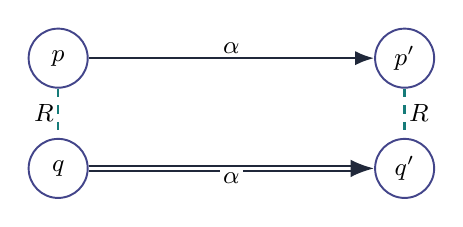
\begin{tikzpicture}[x=1cm,y=1cm]
    \node[st] (p) at (0,1.0) {$p$}; \node[st] (p1) at (4.4,1.0) {$p'$};
    \node[st] (q) at (0,-.4) {$q$}; \node[st] (q1) at (4.4,-.4) {$q'$};
    \draw[trans] (p)--node[lab,above] {$\alpha$}(p1);
    \draw[trans,double,double distance=1pt] (q)--node[lab,below] {$\alpha$}(q1);
    \draw[rel] (p)--node[lab,left] {$R$}(q);
    \draw[rel] (p1)--node[lab,right] {$R$}(q1);
  \end{tikzpicture}
  \par\vspace{1mm}
  {\small Symmetry supplies the same obligation for moves from $q$.}
  \Source{Weak bisimilarity is the greatest weak bisimulation and is an equivalence relation.}
  \note{The union of weak bisimulations is a weak bisimulation. The largest relation is weak bisimilarity and is an equivalence. These facts also follow from the saturation construction in the backup slides.}
\end{frame}


% ----------------------------------------------------------------------
\begin{frame}{Weak Hennessy--Milner logic}
  Recall
  \[
    p\Rightarrow q
    \quad\Longleftrightarrow\quad
    p\step{\tau *}q,
  \]
  and, for $a\in\Sigma$,
  \[
    p\xRightarrow{a}q
    \quad\Longleftrightarrow\quad
    p\step{\tau *}\step{a}\step{\tau *}q.
  \]

  \begin{block}{Weak modalities}
    \[
      \varphi ::= \top
      \mid \neg\varphi
      \mid \varphi\land\psi
      \mid \langle\!\langle\alpha\rangle\!\rangle\varphi,
      \qquad \alpha\in\Sigma\cup\{\tau\}.
    \]
    \[
      p\models\langle\!\langle\alpha\rangle\!\rangle\varphi
      \quad\Longleftrightarrow\quad
      \exists q:\;
      p\xRightarrow{\alpha}q
      \land q\models\varphi .
    \]
    For $\alpha=\tau$, we put $\xRightarrow{\tau}=\Rightarrow$,
    so zero or more internal steps are allowed.
  \end{block}

  \Takeaway{The logic observes the endpoint of a weak transition,
  but not the states crossed by its internal part.}
\end{frame}


% ----------------------------------------------------------------------
\begin{frame}{Weak HML characterizes weak bisimulation}
  \begin{block}{Theorem}
    For finite LTSs,
    \[
      p\approx_{\mathrm w}q
      \quad\Longleftrightarrow\quad
      \forall\varphi\in\mathrm{WHML}:
      \bigl(p\models\varphi\iff q\models\varphi\bigr).
    \]
  \end{block}



  \begin{block}{Why? Saturate the transition system}
    Construct $\mathrm{Sat}(T)$ by putting
    \[
      p\step{a}_{\mathrm w}q
      \quad\Longleftrightarrow\quad
      p\xRightarrow{a}q,  \text{ and }
    \]
    \[
      p\step{\tau}_{\mathrm w}q
      \quad\Longleftrightarrow\quad
      p\Rightarrow q.
    \]
    Then
    \[
      p\approx_{\mathrm w}q\text{ in }T
      \quad\Longleftrightarrow\quad
      p\sim q\text{ in }\mathrm{Sat}(T).
    \]
    Apply the ordinary Hennessy--Milner theorem to $\mathrm{Sat}(T)$.
  \end{block}

  \Takeaway{Weak bisimulation is ordinary bisimulation after forgetting
  the internal structure of finite silent computations.}
  \Source{Hennessy--Milner; De Nicola--Vaandrager.}
\end{frame}


% ----------------------------------------------------------------------
\begin{frame}{What if the logic can inspect a silent computation?}
  Weak HML sees only
  \[
      p \xRightarrow{a} q.
  \]
  It cannot ask what remains possible \emph{while} the silent preparation
  for $a$ is taking place.

  \begin{block}{A CTL-style ``until'' operator}
    Introduce
    \[
      \varphi\langle a\rangle\psi
    \]
    with the semantics
    \[
    p\models\varphi\langle a\rangle\psi
    \]
    iff there exist
    \[
      p=p_0\step{\tau}p_1\step{\tau}\cdots
      \step{\tau}p_n\step{a}q
    \]
    such that
    \[
      p_i\models\varphi\quad(0\leq i\leq n),
      \qquad q\models\psi.
    \]
  \end{block}

  \Takeaway{This is an ``until $a$ happens'' modality:
  it observes properties of the intermediate silent states.}

  \note{This is the essential operator of Hennessy--Milner Logic with Until,
  HMLU. I would call it CTL-style rather than ``weak CTL'', because
  ``CTL over the saturated LTS'' would have different semantics.}
\end{frame}


% ----------------------------------------------------------------------
\begin{frame}{Until can distinguish weakly bisimilar processes}
  Consider
  \[
    R=\tau.a.\nil+b.\nil,
    \qquad
    S=a.\nil+\tau.a.\nil+b.\nil.
  \]

  \begin{columns}[T,onlytextwidth]
    \begin{column}{.46\textwidth}\centering
      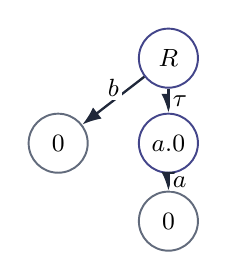
\begin{tikzpicture}[x=1cm,y=.9cm]
        \node[st] (r) at (0,1.2) {$R$};
        \node[st] (r1) at (0,0) {$a.0$};
        \node[terminal] (z1) at (0,-1.1) {$0$};
        \node[terminal] (z2) at (-1.4,0) {$0$};

        \draw[trans] (r)--node[lab,right] {$\tau$}(r1);
        \draw[trans] (r1)--node[lab,right] {$a$}(z1);
        \draw[trans] (r)--node[lab,above] {$b$}(z2);
      \end{tikzpicture}
    \end{column}

    \begin{column}{.50\textwidth}\centering
      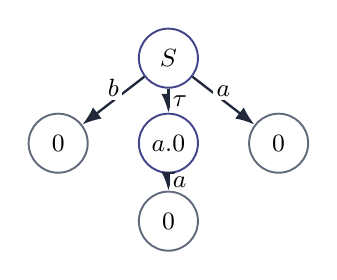
\begin{tikzpicture}[x=1cm,y=.9cm]
        \node[st] (s) at (0,1.2) {$S$};
        \node[st] (s1) at (0,0) {$a.0$};
        \node[terminal] (za) at (1.4,0) {$0$};
        \node[terminal] (zb) at (-1.4,0) {$0$};
        \node[terminal] (z1) at (0,-1.1) {$0$};

        \draw[trans] (s)--node[lab,right] {$\tau$}(s1);
        \draw[trans] (s1)--node[lab,right] {$a$}(z1);
        \draw[trans] (s)--node[lab,above] {$a$}(za);
        \draw[trans] (s)--node[lab,above] {$b$}(zb);
      \end{tikzpicture}
    \end{column}
  \end{columns}

  \[
      R\approx_{\mathrm w}S.
  \]

  But let
  \[
      \chi=
      \bigl(\langle\!\langle b\rangle\!\rangle\top\bigr)
      \langle a\rangle\top.
  \]
  Then
  \[
      S\models\chi,
      \qquad
      R\not\models\chi.
  \]

  \Takeaway{Weak bisimulation forgets too much for an until operator
  that inspects the internal path.}
\end{frame}


% ----------------------------------------------------------------------
\begin{frame}{What exactly does the formula observe?}
  \[
      \chi=
      \bigl(\langle\!\langle b\rangle\!\rangle\top\bigr)
      \langle a\rangle\top.
  \]

  \begin{block}{$S\models\chi$}
    $S$ may perform $a$ immediately:
    \[
       S\step{a}0.
    \]
    Before $a$ happens, we are still in $S$, where $b$ is possible.
  \end{block}

  \begin{alertblock}{$R\not\models\chi$}
    Every execution of $a$ has to start with
    \[
       R\step{\tau}a.0\step{a}0.
    \]
    After the silent step the $b$-alternative has disappeared:
    \[
       a.0\not\models
       \langle\!\langle b\rangle\!\rangle\top.
    \]
  \end{alertblock}

  \Takeaway{The difference is not the visible trace.
  It is \emph{when a branching possibility disappears}.}
\end{frame}


% ----------------------------------------------------------------------
\begin{frame}{Branching bisimulation}
  \begin{block}{Definition}
    A symmetric relation $R$ is a \textbf{branching bisimulation} if
    $p\,R\,q$ and
    \[
       p\step{\alpha}p'
    \]
    imply either
    \[
       \alpha=\tau
       \quad\text{and}\quad p'\,R\,q,
    \]
    or there exist $q_0,q'$ such that
    \[
       q\Rightarrow q_0\step{\alpha}q',
       \qquad
       p\,R\,q_0,
       \qquad
       p'\,R\,q'.
    \]
  \end{block}

  \begin{center}
    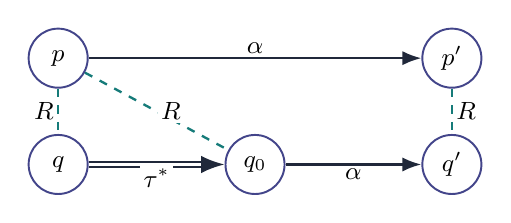
\begin{tikzpicture}[x=1.25cm,y=.9cm]
      \node[st] (p)  at (0,1) {$p$};
      \node[st] (pp) at (4,1) {$p'$};
      \node[st] (q)  at (0,-.5) {$q$};
      \node[st] (q0) at (2,-.5) {$q_0$};
      \node[st] (qp) at (4,-.5) {$q'$};

      \draw[trans] (p)--node[lab,above] {$\alpha$}(pp);
      \draw[trans,double,double distance=1pt]
         (q)--node[lab,below] {$\tau^*$}(q0);
      \draw[trans] (q0)--node[lab,below] {$\alpha$}(qp);
      \draw[rel] (p)--node[lab,left] {$R$}(q);
      \draw[rel] (p)--node[lab,right] {$R$}(q0);
      \draw[rel] (pp)--node[lab,right] {$R$}(qp);
    \end{tikzpicture}
  \end{center}

  \Takeaway{Silent preparation may be ignored only while the original
  branching situation is preserved.}
\end{frame}


% ----------------------------------------------------------------------
\begin{frame}{Weak versus branching bisimulation}
  For the previous processes,
  \[
      R=\tau.a.0+b.0,
      \qquad
      S=a.0+\tau.a.0+b.0,
  \]
  we have
  \[
      R\approx_{\mathrm w}S,
      \qquad
      R\not\approx_{\mathrm b}S.
  \]

  \begin{block}{Why does branching bisimulation fail?}
    Consider the direct transition
    \[
       S\step{a}0.
    \]
    The only way $R$ can prepare an $a$ is
    \[
       R\step{\tau}a.0\step{a}0.
    \]
    Branching bisimulation would require
    \[
       S\approx_{\mathrm b}a.0
    \]
    immediately before the matching $a$.
    This is impossible: $S$ still offers $b$, while $a.0$ does not.
  \end{block}

  \Takeaway{Branching bisimulation remembers which choices survive
  during an internal computation.}
\end{frame}


% ----------------------------------------------------------------------
\begin{frame}{Hennessy--Milner logic with Until}
  \begin{block}{HMLU}
    \[
      \varphi ::=
      \top
      \mid\neg\varphi
      \mid\varphi\land\psi
      \mid\varphi\langle\alpha\rangle\psi .
    \]
    The last operator requires an internal path
    \[
      p=p_0\step{\tau}\cdots\step{\tau}p_n
      \step{\alpha}q
    \]
    such that every $p_i$ satisfies $\varphi$ and $q$ satisfies $\psi$.
  \end{block}

  \begin{block}{Theorem}
    For finite LTSs,
    \[
       p\approx_{\mathrm b}q
       \quad\Longleftrightarrow\quad
       p\text{ and }q\text{ satisfy the same HMLU formulas}.
    \]
  \end{block}

  \[
      \underbrace{\text{weak HML}}_{\text{endpoint only}}
      \quad\leadsto\quad
      \approx_{\mathrm w}
      \qquad
      \underbrace{\text{HMLU}}_{\text{inspect silent prefix}}
      \quad\leadsto\quad
      \approx_{\mathrm b}.
  \]

  \Takeaway{The extra logical power of ``until'' corresponds exactly
  to preservation of branching during silent computation.}
  \Source{De Nicola and Vaandrager, JACM 42(2), 1995.}
\end{frame}


% ----------------------------------------------------------------------
\begin{frame}{Connection with CTL without the next operator}
  HMLU already gives the cleanest action-based characterization.
  There is also a direct connection with CTL.

  \begin{block}{Translate an LTS to a state-labelled system}
    Keep original states and label them by a fresh proposition $\bot$.
    Replace every visible transition
    \[
        p\step{a}q
    \]
    by
    \[
        p\longrightarrow [p,a,q]\longrightarrow q,
    \]
    where the intermediate state is labelled by $a$.
    Silent transitions $p\step{\tau}q$ remain direct edges.
  \end{block}

  \begin{block}{Theorem for finite LTSs}
    Under the divergence-blind interpretation,
    \[
      p\approx_{\mathrm b}q
      \quad\Longleftrightarrow\quad
      p,q\text{ satisfy the same }\mathrm{CTL}^{*}\!-\!X
      \text{ formulas}.
    \]
    In fact, $\mathrm{CTL}-X$ already induces the same equivalence.
  \end{block}

  \Takeaway{Removing $X$ makes finite stuttering invisible,
  while Until still observes whether properties remain true
  throughout the stuttering segment.}
\end{frame}


% ----------------------------------------------------------------------
\begin{frame}{Infinite silence is a separate question}
  Consider
  \[
  \begin{array}{c@{\qquad\qquad}c}
    p\step{a}0
    &
    q\step{a}0,\qquad q\step{\tau}q .
  \end{array}
  \]

  \begin{block}{Ordinary weak and branching bisimulation}
    \[
       p\approx_{\mathrm w}q,
       \qquad
       p\approx_{\mathrm b}q.
    \]
    The $\tau$-loop can be ignored forever.
  \end{block}

  \begin{alertblock}{But there is an observable design question}
    $q$ admits an infinite internal computation
    \[
       q\step{\tau}q\step{\tau}q\step{\tau}\cdots,
    \]
    while $p$ does not.
  \end{alertblock}

  If this distinction matters, use a
  \textbf{divergence-preserving} version of the equivalence
  (and a corresponding divergence-sensitive logic).

  \Takeaway{Two independent questions arise:
  what may finite silent computation forget, and whether infinite silence matters.}
\end{frame}


% ----------------------------------------------------------------------
\begin{frame}{Weak and branching bisimilarity are not congruences}
  Both equivalences abstract from an initial finite silent computation:
  \[
       \tau.0\approx_{\mathrm w}0,
       \qquad
       \tau.0\approx_{\mathrm b}0.
  \]

  Now put the processes in the choice context
  \[
       C[-]=a.0+[-].
  \]

  Then
  \[
      C[\tau.0]=a.0+\tau.0,
      \qquad
      C[0]=a.0+0.
  \]

  But
  \[
      a.0+\tau.0\not\approx_{\mathrm w}a.0+0.
  \]
  The left process can silently choose the second branch and deadlock,
  while the right process cannot.

  Hence also
  \[
      a.0+\tau.0\not\approx_{\mathrm b}a.0+0.
  \]

  \Takeaway{The problem is at the root:
  an initial silent step may resolve an external choice.}
\end{frame}


% ----------------------------------------------------------------------
\begin{frame}{Rooted weak bisimilarity}
  To recover substitution under choice, treat the first move more strictly.

  Define
  \[
  q\xRightarrow{\widehat{\alpha}}q'=
  \begin{cases}
    q\Rightarrow\step{a}\Rightarrow q',
       & \alpha=a\in\Sigma,\\[1mm]
    q\Rightarrow\step{\tau}\Rightarrow q',
       & \alpha=\tau.
  \end{cases}
  \]
  Notice that a root $\tau$ must now be matched by
  \textbf{at least one} $\tau$.

  \begin{block}{Rooted weak bisimilarity}
    \[
      p\approx_{\mathrm{rw}}q
    \]
    iff every initial
    \[
      p\step{\alpha}p'
    \]
    can be matched by
    \[
      q\xRightarrow{\widehat{\alpha}}q'
      \qquad\text{with}\qquad
      p'\approx_{\mathrm w}q',
    \]
    and symmetrically.
  \end{block}

  Thus
  \[
     \tau.0\not\approx_{\mathrm{rw}}0.
  \]

  \Takeaway{After the root has been matched, ordinary weak
  bisimilarity is sufficient again.}
\end{frame}


% ----------------------------------------------------------------------
\begin{frame}{Rooted branching bisimilarity}
  For branching bisimulation the standard root condition is even cleaner.

  \begin{block}{Definition}
    \[
       p\approx_{\mathrm{rb}}q
    \]
    iff every initial transition
    \[
       p\step{\alpha}p'
    \]
    can be matched by an actual transition
    \[
       q\step{\alpha}q'
    \]
    such that
    \[
       p'\approx_{\mathrm b}q',
    \]
    and symmetrically.
  \end{block}

  \begin{block}{Compositional role}
    The rooted variants repair the failure under nondeterministic choice.
    For the standard CCS-style operators they give the corresponding
    congruences.
  \end{block}

  \Takeaway{Rootedness and branching preservation solve different problems:
  branching controls what may happen \emph{inside} a silent computation;
  rootedness controls how a component may be used by its environment.}
\end{frame}


% ----------------------------------------------------------------------
\begin{frame}{What $\tau$ adds to the picture}
  \begin{center}
  \renewcommand{\arraystretch}{1.45}
  \begin{tabular}{@{}lll@{}}
    \textbf{Observation} &
    \textbf{Logic} &
    \textbf{Equivalence}\\
    \hline
    every transition &
    HML &
    strong bisimulation\\

    endpoints of silent computations &
    weak HML &
    weak bisimulation\\

    branching preserved during silence &
    HML with Until &
    branching bisimulation\\

    finite stuttering in branching time &
    CTL$^{*}{-}X$ &
    branching bisimulation\\
  \end{tabular}
  \end{center}

  \vspace{4mm}

  Two additional refinements answer independent questions:
  \[
      \text{divergence preservation}
      \qquad\text{and}\qquad
      \text{rootedness / congruence}.
  \]

  \Takeaway{There is no single way to ``ignore $\tau$'':
  the equivalence depends on what the observer is allowed to see.}
\end{frame}

% 18 -----------------------------------------------------------------
\begin{frame}{First example: an internal delay}
  \[
    P=a.\nil,\qquad Q=\tau.a.\nil.
  \]
  \centering
  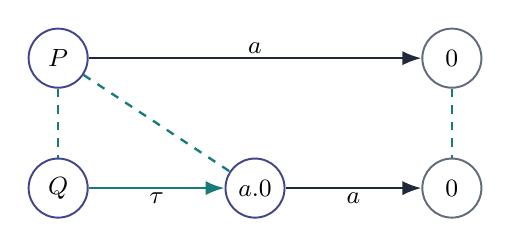
\begin{tikzpicture}[x=1cm,y=1cm]
    \node[st] (p) at (0,1.05) {$P$}; \node[terminal] (p0) at (5,1.05) {$0$};
    \node[st] (q) at (0,-.6) {$Q$}; \node[st] (q1) at (2.5,-.6) {$a.0$};
    \node[terminal] (q0) at (5,-.6) {$0$};
    \draw[trans] (p)--node[lab,above] {$a$}(p0);
    \draw[tauedge] (q)--node[lab,below] {$\tau$}(q1);
    \draw[trans] (q1)--node[lab,below] {$a$}(q0);
    \draw[rel] (p)--(q); \draw[rel] (p)--(q1); \draw[rel] (p0)--(q0);
  \end{tikzpicture}
  \par\vspace{1mm}
  \uncover<2->{\Takeaway{$P\wb Q$, but $P\not\sim Q$. The $\tau$-step of $Q$ can be matched by $P$ doing nothing.}}
  \note{The two displayed states named a.0/P have identical behaviour; the dotted links show a possible witness across disjoint copies. All displayed zero states are deadlocks.}
\end{frame}

% 19 -----------------------------------------------------------------
\begin{frame}{Weak bisimulation detects silent deadlock}
  Return to $P=a.\nil+\tau.\nil$ and $Q=a.\nil$.
  \begin{block}{The missing obligation is now present}
    If $P\,R\,Q$ and $P\step{\tau}\nil$, we need
    \[
      Q\silent Q'\quad\text{and}\quad\nil\,R\,Q'.
    \]
    $Q$ has no internal move, so $Q'=Q$.
    But $Q$ can perform $a$, and $\nil$ cannot match it.
  \end{block}
  Therefore $P\notwb Q$.
  \begin{exampleblock}{What is intentionally ignored}
    $\tau.\nil\wb\nil$: finite internal work leading only to inaction adds no visible possibility.

  \end{exampleblock}
  \Takeaway{Ignore the duration of finite internal work, not its effect on the available continuations.}
\end{frame}

% 20 -----------------------------------------------------------------
\section{Branching bisimulation}
\begin{frame}{Weak matching may pass over a choice}
  \centering
  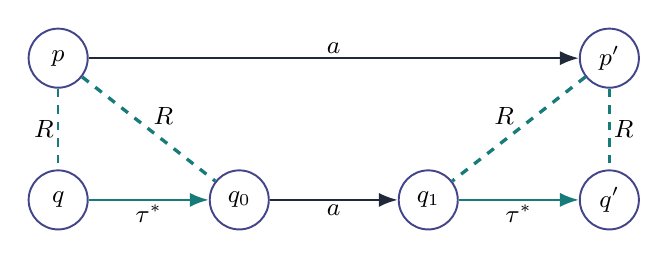
\begin{tikzpicture}[x=1cm,y=1cm]
    \node[st] (p) at (0,1.3) {$p$}; \node[st] (pp) at (7,1.3) {$p'$};
    \node[st] (q) at (0,-.5) {$q$}; \node[st] (q0) at (2.3,-.5) {$q_0$};
    \node[st] (q1) at (4.7,-.5) {$q_1$}; \node[st] (qq) at (7,-.5) {$q'$};
    \draw[trans] (p)--node[lab,above] {$a$}(pp);
    \draw[tauedge] (q)--node[lab,below] {$\tau^*$}(q0);
    \draw[trans] (q0)--node[lab,below] {$a$}(q1);
    \draw[tauedge] (q1)--node[lab,below] {$\tau^*$}(qq);
    \draw[rel] (p)--node[lab,left] {$R$}(q);
    \draw[rel] (pp)--node[lab,right] {$R$}(qq);
    \uncover<2->{\draw[rel,line width=1.2pt] (p)--node[lab,above right] {$R$}(q0);
      \draw[rel,line width=1.2pt] (pp)--node[lab,above left] {$R$}(q1);}
  \end{tikzpicture}
  \par\vspace{4mm}
  \begin{block}{Weak bisimulation}
    Requires related endpoints; no explicit obligations at $q_0$ and $q_1$.
  \end{block}
  \uncover<2->{\Takeaway{Branching bisimulation also preserves the choices \emph{around} the matching visible action. We use an equivalent definition with no trailing silent path.}}
  \Source{Adapted matching diagram from \cite{GW96}; the next slide uses the formulation of \cite{GLT09}.}
\end{frame}

% 21 -----------------------------------------------------------------
\begin{frame}{Branching bisimulation: definition}
  Write $u\optstep{\alpha}v$ for a single $\alpha$-step, or for $u=v$ when $\alpha=\tau$.
  \begin{block}{Definition}
    A symmetric relation $R$ is a \textbf{branching bisimulation} if
    $p\,R\,q$ and $p\step{\alpha}p'$ imply that there exist $q_0,q'$ with
    \[
      q\silent q_0\optstep{\alpha}q',
      \qquad \boxed{p\,R\,q_0},\qquad p'\,R\,q'.
    \]
    We write $p\bb q$ if some branching bisimulation relates them.
  \end{block}
  \begin{itemize}\setlength\itemsep{2mm}
    \item Before the matching action, $q_0$ must still represent $p$.
    \item Immediately afterwards, $q'$ must represent $p'$.
    \item A $\tau$-step may be ignored only when the required states remain related.
  \end{itemize}
  \Source{\cite[Definition 2.1]{GLT09}. Branching bisimilarity is an equivalence relation.}
  \note{This is the optional-final-step relational definition from GLT09, which induces standard branching bisimilarity. Do not insist that every tau-transition must be inert. For the largest relation, the stuttering property ensures that the preparatory tau path stays in the source equivalence class.}
\end{frame}

% 22 -----------------------------------------------------------------
\begin{frame}{Weak, but not branching, bisimilar}
  \[
    X=b.\nil+\tau.C,\quad C=c.\nil,\qquad
    P=a.X,\quad Q=a.X+a.C.
  \]
  \centering
  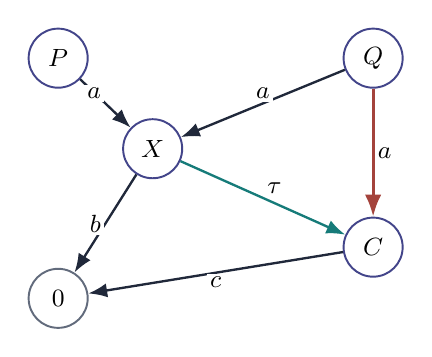
\begin{tikzpicture}[x=1cm,y=1cm]
    \node[st] (p) at (-2,1.05) {$P$};
    \node[st] (q) at (2,1.05) {$Q$};
    \node[st] (x) at (-.8,-.1) {$X$};
    \node[st] (c) at (2,-1.35) {$C$};
    \node[terminal] (z) at (-2,-2.0) {$0$};
    \draw[trans] (p)--node[lab,above left] {$a$}(x);
    \draw[trans] (q)--node[lab,above] {$a$}(x);
    \draw[newedge] (q)--node[lab,right] {$a$}(c);
    \draw[tauedge] (x)--node[lab,above right] {$\tau$}(c);
    \draw[trans] (x)--node[lab,left] {$b$}(z);
    \draw[trans] (c)--node[lab,below] {$c$}(z);
  \end{tikzpicture}
  \par\vspace{1mm}
  \Takeaway{$P\wb Q$, but $P\notbb Q$: the additional transition bypasses $X$, where $b$ is still possible.}
  \note{This is a compact instance of the standard weak tau-law a.(B+tau.C)+a.C approximately a.(B+tau.C). Share X, C and 0 between the two roots, so the weak witness consists of identity pairs plus (P,Q) and its converse.}
\end{frame}

% 23 -----------------------------------------------------------------
\begin{frame}{The separating example: why the relations differ}
  \[
    P=a.X,\quad Q=a.X+a.C,\quad X=b.\nil+\tau.C,\quad C=c.\nil.
  \]
  \begin{columns}[T,onlytextwidth]
    \begin{column}{.48\textwidth}
      \begin{exampleblock}{Weak: $P\wb Q$}
        Match the additional move $Q\step{a}C$ by
        \[
          P\step{a}X\step{\tau}C.
        \]
        Other moves match directly.\\[1mm]
        A witness is
        \[
          R=\Id\cup\{(P,Q),(Q,P)\}.
        \]
      \end{exampleblock}
    \end{column}
    \begin{column}{.48\textwidth}
      \begin{alertblock}{Branching: $P\notbb Q$}
        $P$ has no initial $\tau$-step. Matching $Q\step{a}C$ must therefore use
        \[
          P\step{a}X.
        \]
        This requires $X\bb C$, but only $X$ can perform $b$.
      \end{alertblock}
    \end{column}
  \end{columns}
  \Takeaway{Weak matching may combine the $a$-step with discarding $b$. Branching matching cannot.}
\end{frame}

% 24 -----------------------------------------------------------------
\begin{frame}{Why prefer branching bisimulation?}
  For a visible step $p\step{a}p'$, a branching response can be chosen as
  \[
    \begin{gathered}
      q=q_0\step{\tau}q_1\step{\tau}\cdots\step{\tau}q_k\step{a}q',\\[1mm]
      \boxed{p\bb q_i\quad(0\leq i\leq k)},\qquad p'\bb q'.
    \end{gathered}
  \]
  \begin{block}{Internal preparation stays in one abstract state}
    Every $q_i$ represents $p$. Immediately after the matching visible step,
    $q'$ represents $p'$.
  \end{block}
  \begin{exampleblock}{Contrast with weak matching}
    Only the endpoints must be related. Internal preparation and completion
    may pass through other behaviours.
  \end{exampleblock}
  \Takeaway{Branching equivalence preserves more intermediate structure. Divergence preservation and rootedness remain separate requirements.}
  \vspace{-2mm}\Source{Branching transfer and the stuttering property: \cite{GW96,GLT09}.}
  \note{For the largest branching equivalence, both ends of the preparatory path are equivalent to p. The stuttering property puts every intermediate state in that class. Do not present the bare endpoint stuttering property alone as a separator from weak bisimilarity: the extra transfer obligations are decisive. Weak bisimulation remains a legitimate coarser observation regime.}
\end{frame}

% 25 -----------------------------------------------------------------
\begin{frame}{Three equivalences, three levels of abstraction}
  \[
    {\sim}\ \subsetneq\ {\approx_{\mathrm b}}\ \subsetneq\ {\approx_{\mathrm w}}.
  \]
  \vspace{3mm}
  \renewcommand{\arraystretch}{1.6}
  \begin{tabular}{@{}p{.27\textwidth}p{.67\textwidth}@{}}
    \textbf{Strong} & Match one transition by one transition.\\
    \textbf{Branching} & Abstract from internal steps while preserving branching during matching.\\
    \textbf{Weak} & Match transitions by weak paths with related endpoints.
  \end{tabular}
  \vspace{2mm}
  \begin{block}{Witnesses for strictness}
    $a.\nil\bb\tau.a.\nil$, but they are not strongly bisimilar.\\[1mm]
    The previous $P,Q$ are weakly, but not branching, bisimilar.
  \end{block}
  \Source{On LTSs without $\tau$-transitions, all three notions coincide. See \cite{GW96}.}
  \note{Branching implies weak directly: the branching response is a legal weak response. For an optional tau final step this is still a tau-star path. No claim about a partial-order or true-concurrency semantics is being made.}
\end{frame}

% 26 -----------------------------------------------------------------
\section{Divergence}
\begin{frame}{Divergence: silent activity may continue forever}
  \begin{block}{Definition}
    A state $p$ \textbf{diverges} if there is an infinite execution
    \[
      p=p_0\step{\tau}p_1\step{\tau}p_2\step{\tau}\cdots.
    \]
  \end{block}
  \centering
  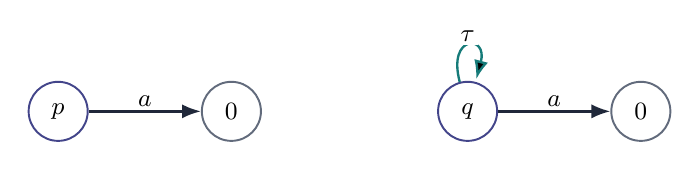
\begin{tikzpicture}[x=1cm,y=1cm]
    \node[st] (p) at (0,0) {$p$}; \node[terminal] (z1) at (2.2,0) {$0$};
    \node[st] (q) at (5.2,0) {$q$}; \node[terminal] (z2) at (7.4,0) {$0$};
    \draw[trans] (p)--node[lab,above] {$a$}(z1);
    \draw[trans] (q)--node[lab,above] {$a$}(z2);
    \draw[tauedge] (q) edge[loop above] node[lab] {$\tau$} (q);
  \end{tikzpicture}
  \par\vspace{2mm}
  \uncover<2->{\Takeaway{$p\bb q$, yet only $q$ has an infinite execution avoiding $a$.}}
  \Source{For maximal executions, with no fairness assumption. Infinite activity is not a deadlock.}
\end{frame}

% 27 -----------------------------------------------------------------
\begin{frame}{Finite silence, deadlock, and infinite silence}
  Let $D$ have only the self-loop $D\step{\tau}D$.
  \begin{block}{Ordinary weak and branching bisimilarity}
    \[
      \nil\bb\tau.\nil\bb D.
    \]
    All three have no visible behaviour, but only $D$ has infinite internal activity.
  \end{block}
  \begin{exampleblock}{Divergence-preserving branching bisimilarity}
    Add an obligation to match infinite internal activity within related behaviour.
    Then
    \[
      \nil\dbb\tau.\nil,\qquad \nil\notdbb D.
    \]
  \end{exampleblock}
  \Takeaway{Divergence preservation distinguishes infinite activity from finite silence. It does not make every internal step observable.}
  \Source{\cite{GLT09}. No fairness assumption is implicit; the exact divergence clause is in the appendix.}
  \note{A deadlock has no outgoing transition. An internal loop is not a deadlock, even though it may provide no visible progress. Ordinary weak and branching equivalence ignore this distinction in the pure-loop example. The previous example with an a-exit explains why this matters for inevitable response. Do not claim preservation of arbitrary CTL formulas or arbitrary fairness assumptions.}
\end{frame}

% 28 -----------------------------------------------------------------
\section{Rooted relations}
\begin{frame}{Ordinary weak equivalences fail under choice}
  \[
    P=\tau.a.\nil\bb a.\nil=Q,\qquad C[-]=[-]+b.\nil.
  \]
  \begin{columns}[T,onlytextwidth]
    \begin{column}{.49\textwidth}\centering
      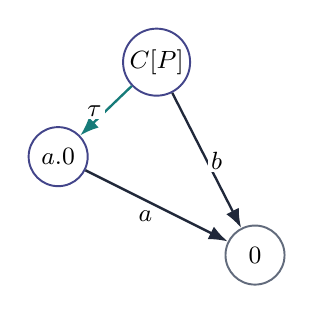
\begin{tikzpicture}[x=1cm,y=1cm]
        \node[st] (p) at (0,1.0) {$C[P]$};
        \node[st] (a) at (-1.25,-.2) {$a.0$};
        \node[terminal] (z) at (1.25,-1.45) {$0$};
        \draw[tauedge] (p)--node[lab,left] {$\tau$}(a);
        \draw[trans] (p)--node[lab,right] {$b$}(z);
        \draw[trans] (a)--node[lab,below left] {$a$}(z);
      \end{tikzpicture}
    \end{column}
    \begin{column}{.49\textwidth}\centering
      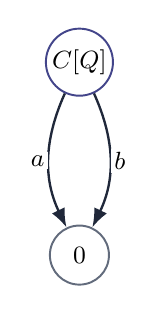
\begin{tikzpicture}[x=1cm,y=1cm]
        \node[st] (q) at (0,1.0) {$C[Q]$};
        \node[terminal] (z) at (0,-1.45) {$0$};
        \draw[trans] (q) to[bend right=25] node[lab,left] {$a$} (z);
        \draw[trans] (q) to[bend left=25] node[lab,right] {$b$} (z);
      \end{tikzpicture}
    \end{column}
  \end{columns}
  \uncover<2->{\Takeaway{$C[P]\notwb C[Q]$, hence also $C[P]\notbb C[Q]$. The left process can silently discard $b$; the right process cannot.}}
  \Source{The weak-choice counterexample from the supplied slides, made explicit.}
\end{frame}

% 29 -----------------------------------------------------------------
\begin{frame}{The coarsest congruence contained in an equivalence}
  Starting with an equivalence $\approx$, define
  \[
    P\approx^{\mathrm{ctx}}Q
    \quad\Longleftrightarrow\quad
    \forall C[-]:\ C[P]\approx C[Q].
  \]
  \begin{block}{Why this is the desired repair}
    \begin{itemize}\setlength\itemsep{2mm}
      \item The identity context gives $\approx^{\mathrm{ctx}}\,\subseteq\,\approx$.
      \item Composing contexts shows that $\approx^{\mathrm{ctx}}$ is a congruence.
      \item Every congruence contained in $\approx$ is contained in $\approx^{\mathrm{ctx}}$.
    \end{itemize}
  \end{block}
  \Takeaway{Root conditions give a local characterisation, avoiding quantification over all contexts.}
  \Source{For the usual CCS setting, root conditions provide such characterisations; see \cite{MCS}.}
  \note{The claim that contextual refinement is an equivalence is pointwise inherited from the base equivalence. Closure of our one-hole contexts under composition proves compatibility. 'Coarsest' means largest as a relation among congruences contained in the base equivalence.}
\end{frame}

% 30 -----------------------------------------------------------------
\begin{frame}{Rooted branching bisimilarity}
  \begin{block}{Definition}
    $P\rbb Q$ if every transition $P\step{\alpha}P'$ has a match
    \[
      Q\step{\alpha}Q'\quad\text{with}\quad P'\bb Q',
    \]
    and conversely, for every $\alpha\in\Act$.
  \end{block}
  \Takeaway{Match the initial step \textbf{strictly}, including $\tau$; compare successors by \textbf{ordinary branching bisimilarity}.}
  \[
    \tau.a.\nil\notrbb a.\nil,
    \qquad
    a.\tau.b.\nil\rbb a.b.\nil.
  \]
  {\small\textcolor{Warn}{Do not require rooted equivalence of the successors:} that would impose strong-style matching at every step.}
  \Source{Root conditions: \cite{MCS,GLS20}.}
\end{frame}

% 31 -----------------------------------------------------------------
\begin{frame}{Rooted weak bisimilarity: a different root condition}
  \begin{block}{Definition: observational congruence}
    $P\rwb Q$ if every $P\step{\alpha}P'$ can be matched by
    \[
      Q\silent Q_0\step{\alpha}Q_1\silent Q'
      \quad\text{with}\quad P'\wb Q',
    \]
    and symmetrically, for all $\alpha\in\Act$.
  \end{block}
  \begin{alertblock}{The middle step is compulsory, also for $\alpha=\tau$}
    Matching an initial $\tau$ requires at least one $\tau$-transition: $\tau^+$, not merely $\tau^*$.
  \end{alertblock}
  \renewcommand{\arraystretch}{1.45}
  \begin{tabular}{@{}ll@{}}
    Rooted branching: & one initial step; branching-equivalent successors.\\
    Rooted weak: & a nonempty matching weak path; weak-equivalent successors.
  \end{tabular}
  \Source{\cite{MCS}. Both are congruences for the constructors used in the lecture.}
\end{frame}

% 32 -----------------------------------------------------------------
\begin{frame}{Rootedness repairs the choice problem}
  \begin{block}{Theorem}
    Rooted branching and rooted weak bisimilarity are congruences for prefix, choice, blocking, and hiding.
  \end{block}
  \textbf{Choice case.} Assume $P\rbb Q$ and consider $P+R$ and $Q+R$.
  \begin{itemize}\setlength\itemsep{2.5mm}
    \item If $P+R\step{\alpha}P'$ uses $P$, rootedness provides
      $Q\step{\alpha}Q'$ with $P'\bb Q'$. Thus $Q+R$ has the required \emph{single} matching step.
    \item If the move uses $R$, use the identical step of $R$ on the other side.
  \end{itemize}
  \Takeaway{Once the first transition has resolved the choice, ordinary branching equivalence suffices for the derivatives.}
  \Source{\cite{MCS}. For rooted weak equivalence, a nonempty response also resolves the outer choice; a zero-step response would not.}
  \note{For prefix, use P approximately_b Q, implied by rootedness. For parallel, the immediate step is either a component step or a synchronisation, and the derivative pair is branching equivalent by compatibility of branching equivalence with parallel. Restriction and hiding preserve the matching label, and the derivative pair remains branching equivalent.}
\end{frame}

% 33 -----------------------------------------------------------------
\begin{frame}{Rootedness and divergence solve different problems}
  \renewcommand{\arraystretch}{1.55}
  \begin{tabular}{@{}p{.26\textwidth}p{.68\textwidth}@{}}
    \textbf{Rootedness} & Protects initial branching when a component is placed in a context.\\
    \shortstack[l]{\textbf{Divergence}\\\textbf{preservation}} & Prevents infinite internal activity from being erased by equivalence.
  \end{tabular}
  \vspace{3mm}
  Let $D$ have only the self-loop $D\step{\tau}D$. Then
  \[
    a.\nil\rbb a.D,
    \qquad\text{but}\qquad a.\nil\notdbb a.D.
  \]
  \uncover<2->{\begin{block}{The other direction also fails}
    \[
      a.\nil\dbb\tau.a.\nil,
      \qquad a.\nil\notrbb\tau.a.\nil.
    \]
  \end{block}}
  \Takeaway{The two refinements are incomparable. They can also be combined.}
  \note{First example: 0 and D are branching equivalent, so strict matching of the initial a succeeds. However D diverges and 0 does not. Second example: both processes are divergence-free and branching equivalent but the roots have different immediate labels. Rooted divergence-preserving branching bisimilarity uses approximately_b^Delta for the derivatives in the rooted definition.}
\end{frame}

% 34 -----------------------------------------------------------------
\section{Compositional application}
\begin{frame}{Application: extend the language with communication}
  Visible actions come in complementary pairs $a,\bar a$, with $\overline{\bar a}=a$.
  Only complementary visible actions synchronise.
  \begin{block}{A component can move on its own}
    \[
      \frac{P\step{\alpha}P'}{P\parallel Q\step{\alpha}P'\parallel Q}
      \qquad
      \frac{Q\step{\alpha}Q'}{P\parallel Q\step{\alpha}P\parallel Q'}.
    \]
  \end{block}
  \begin{block}{Two components can communicate}
    \[
      \frac{P\step{a}P'\qquad Q\step{\bar a}Q'}
           {P\parallel Q\step{\tau}P'\parallel Q'}.
    \]
  \end{block}
  \Takeaway{Synchronisation is possible, but not compulsory. Blocking both $a$ and $\bar a$ forces a private handshake.}
  \Source{Add parallel contexts $C[-]\parallel R$ and $R\parallel C[-]$. Strong and rooted congruence extend to them \cite{MCS}.}
\end{frame}

% 35 -----------------------------------------------------------------
\begin{frame}{An internal handshake gives a replaceable implementation}
  \[
    \begin{aligned}
      \mathit{Client}&=\mathsf{req}.\bar h.\mathsf{done}.\nil,&
      \mathit{Server}&=h.\nil,\\
      \mathit{System}&=\blockact{\{h,\bar h\}}{\mathit{Client}\parallel\mathit{Server}},&
      \mathit{Spec}&=\mathsf{req}.\mathsf{done}.\nil.
    \end{aligned}
  \]
  \centering
  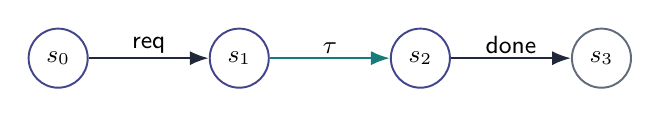
\begin{tikzpicture}[x=1cm,y=1cm]
    \node[st] (s0) at (0,0) {$s_0$}; \node[st] (s1) at (2.3,0) {$s_1$};
    \node[st] (s2) at (4.6,0) {$s_2$}; \node[terminal] (s3) at (6.9,0) {$s_3$};
    \draw[trans] (s0)--node[lab,above] {$\mathsf{req}$}(s1);
    \draw[tauedge] (s1)--node[lab,above] {$\tau$}(s2);
    \draw[trans] (s2)--node[lab,above] {$\mathsf{done}$}(s3);
  \end{tikzpicture}
  \par\vspace{2mm}
  \begin{block}{What blocking enforces}
    The $h$ and $\bar h$ actions cannot occur separately. Their joint transition is labelled $\tau$ and is not blocked.
  \end{block}
  \Takeaway{$\mathit{System}\rbb\mathit{Spec}$. Both start with $\mathsf{req}$; their derivatives are branching bisimilar.}
  \note{Let H={h,bar h}. Then s1=block_H(bar h.done.0 || h.0), s2=block_H(done.0 || 0), and s3=block_H(0 || 0). The req transitions match strictly; their derivatives are branching equivalent via the single internal handshake. Thus the systems are rooted branching equivalent and can be substituted in the extended finite contexts.}
\end{frame}

% 36 -----------------------------------------------------------------
\section{Confluence}
\begin{frame}{Confluence: different paths can be joined}
  For a binary reduction relation $\to_r$, \textbf{confluence} means
  \[
    s\step{r*}u\ \land\ s\step{r*}v
    \quad\Longrightarrow\quad
    \exists w:\ u\step{r*}w\ \land\ v\step{r*}w.
  \]
  \centering
  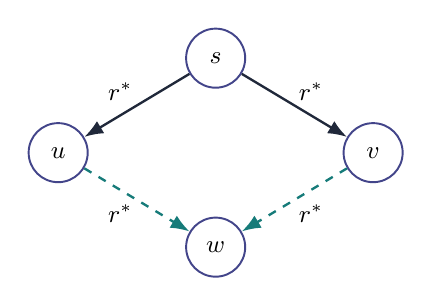
\begin{tikzpicture}[x=1cm,y=1cm]
    \node[st] (s) at (0,1.2) {$s$};
    \node[st] (u) at (-2,0) {$u$}; \node[st] (v) at (2,0) {$v$};
    \node[st] (w) at (0,-1.2) {$w$};
    \draw[trans] (s)--node[lab,above left] {$r^*$}(u);
    \draw[trans] (s)--node[lab,above right] {$r^*$}(v);
    \draw[tauedge,dashed] (u)--node[lab,below left] {$r^*$}(w);
    \draw[tauedge,dashed] (v)--node[lab,below right] {$r^*$}(w);
  \end{tikzpicture}
  \par\vspace{1mm}
  \Takeaway{For behavioural abstraction, joining internal paths is not enough: visible alternatives must also be respected.}
  \note{Only introduce the joining idea. Do not claim local confluence implies confluence without termination. The remaining slides use a local tau-focused sufficient condition from Groote and van de Pol, not the full CCS weak-confluence notion in the old slides.}
\end{frame}

% 37 -----------------------------------------------------------------
\begin{frame}{Internal confluence alone is insufficient}
  Return to
  \[
    S=\tau.a.\nil+b.\nil.
  \]
  Its $\tau$-relation is terminating and confluent: there is only one internal edge.
  \begin{columns}[T,onlytextwidth]
    \begin{column}{.43\textwidth}\centering
      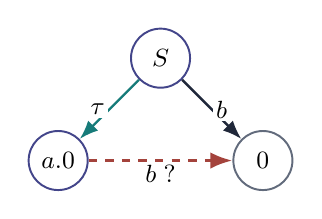
\begin{tikzpicture}[x=1cm,y=1cm]
        \node[st] (s) at (0,1.0) {$S$};
        \node[st] (a) at (-1.3,-.3) {$a.0$};
        \node[terminal] (z) at (1.3,-.3) {$0$};
        \draw[tauedge] (s)--node[lab,left] {$\tau$}(a);
        \draw[trans] (s)--node[lab,right] {$b$}(z);
        \draw[newedge,dashed] (a)--node[lab,below] {$b\;?$}(z);
      \end{tikzpicture}
    \end{column}
    \begin{column}{.54\textwidth}
      \begin{alertblock}{The missing matching behaviour}
        After the $\tau$-step, $b$ is unavailable.\\[2mm]
        Therefore $S\notbb a.\nil$.
      \end{alertblock}
    \end{column}
  \end{columns}
  \Takeaway{To prioritise an internal step, check its interaction with \emph{all competing labels}, not only $\tau$.}
\end{frame}

% 38 -----------------------------------------------------------------
\begin{frame}{A local sufficient condition: $T$-confluence}
  Choose a set $T$ of internal transitions. Write $s\step{\tau}_T t$ for an edge in $T$.
  \begin{block}{Definition}
    For every $s\step{\tau}_T t$ and $s\step{\alpha}u$, there is $v$ such that
    \[
      t\optstep{\alpha}v
      \quad\text{and}\quad
      u=v\ \text{or}\ u\step{\tau}_T v.
    \]
  \end{block}
  \begin{columns}[c,onlytextwidth]
    \begin{column}{.45\textwidth}\centering
      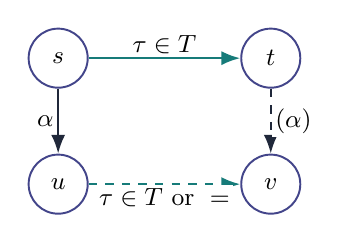
\begin{tikzpicture}[x=1cm,y=1cm]
        \node[st] (s) at (0,1.15) {$s$}; \node[st] (t) at (2.7,1.15) {$t$};
        \node[st] (u) at (0,-.45) {$u$}; \node[st] (v) at (2.7,-.45) {$v$};
        \draw[tauedge] (s)--node[lab,above] {$\tau\in T$}(t);
        \draw[trans] (s)--node[lab,left] {$\alpha$}(u);
        \draw[tauedge,dashed] (u)--node[lab,below] {$\tau\in T\ \text{or }=$}(v);
        \draw[trans,dashed] (t)--node[lab,right] {$(\alpha)$}(v);
      \end{tikzpicture}
    \end{column}
    \begin{column}{.52\textwidth}
      The right-hand step is optional only for $\alpha=\tau$.\\[2mm]
      The bottom edge, when present, must belong to the \emph{same set} $T$.
    \end{column}
  \end{columns}
  \Source{\cite[Section 2]{GP00}. This local reduction criterion is not the full CCS confluence notion.}
\end{frame}

% 39 -----------------------------------------------------------------
\begin{frame}{Confluent internal steps are inert}
  \begin{block}{Theorem}
    If the LTS is $T$-confluent, then
    \[
      s\step{\tau}_T t\quad\Longrightarrow\quad s\bb t.
    \]
    Such an internal transition is called \textbf{inert}.
  \end{block}
  \textbf{Proof idea.} Consider
  \[
    R=\Id\cup T\cup T^{-1},
  \]
  viewing $T$ as a relation on its endpoints.
  \begin{itemize}\setlength\itemsep{2mm}
    \item Match a move from $s$ using the confluence square.
    \item Match a move from $t$ by first taking $s\step{\tau}_T t$, then copying it.
  \end{itemize}
  \Takeaway{This local confluence criterion is sufficient for inertness, but not necessary.}
  \Source{\cite[Section 2]{GP00}. This inertness theorem does not require termination.}
\end{frame}

% 40 -----------------------------------------------------------------
\begin{frame}{Prioritising internal work}
  \begin{block}{A sound reduction under an explicit assumption}
    Suppose the LTS is $T$-confluent and \textbf{$\tau$-convergent}: it has no infinite $\tau$-execution. At each state with an outgoing $T$-edge, retain one such edge and remove its other outgoing transitions.
  \end{block}
  \centering
  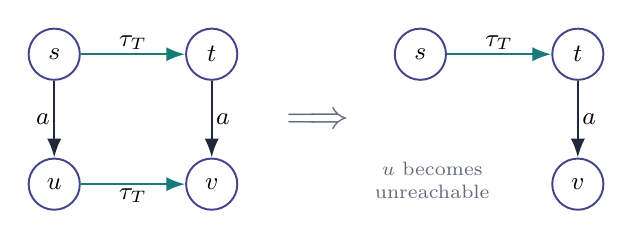
\begin{tikzpicture}[x=1cm,y=1cm,st/.append style={minimum size=6.5mm}]
    \node[st] (s) at (0,1.05) {$s$}; \node[st] (t) at (2,1.05) {$t$};
    \node[st] (u) at (0,-.6) {$u$}; \node[st] (v) at (2,-.6) {$v$};
    \draw[tauedge] (s)--node[lab,above] {$\tau_T$}(t);
    \draw[trans] (s)--node[lab,left] {$a$}(u);
    \draw[trans] (t)--node[lab,right] {$a$}(v);
    \draw[tauedge] (u)--node[lab,below] {$\tau_T$}(v);
    \node[font=\Large,text=Muted] at (3.35,.2) {$\Longrightarrow$};
    \node[st] (s2) at (4.65,1.05) {$s$}; \node[st] (t2) at (6.65,1.05) {$t$};
    \node[st] (v2) at (6.65,-.6) {$v$};
    \draw[tauedge] (s2)--node[lab,above] {$\tau_T$}(t2);
    \draw[trans] (t2)--node[lab,right] {$a$}(v2);
    \node[font=\scriptsize,text=Muted,align=center] at (4.8,-.55) {$u$ becomes\\unreachable};
  \end{tikzpicture}
  \par\vspace{1mm}
  \Takeaway{The initial states remain branching bisimilar. Removing unreachable states can shrink the graph before full minimisation.}
  \Source{\cite[Section 5]{GP00}. The guarantee is ordinary branching bisimilarity, not rooted equivalence.}
\end{frame}

% 41 -----------------------------------------------------------------
\begin{frame}{Why the convergence assumption matters}
  \centering
  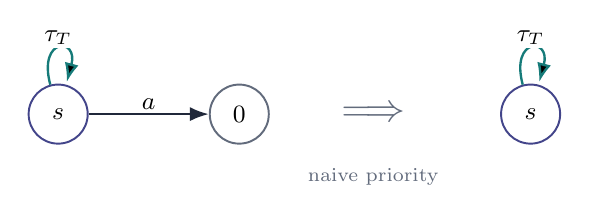
\begin{tikzpicture}[x=1cm,y=1cm]
    \node[st] (s) at (0,0) {$s$}; \node[terminal] (z) at (2.3,0) {$0$};
    \draw[tauedge] (s) edge[loop above] node[lab] {$\tau_T$} (s);
    \draw[trans] (s)--node[lab,above] {$a$}(z);
    \node[text=Muted,font=\Large] at (4,0) {$\Longrightarrow$};
    \node[st] (s2) at (6,0) {$s$};
    \draw[tauedge] (s2) edge[loop above] node[lab] {$\tau_T$} (s2);
    \node[font=\scriptsize,text=Muted] at (4,-.8) {naive priority};
  \end{tikzpicture}
  \par\vspace{4mm}
  \begin{alertblock}{The self-loop is confluent, but the reduction is wrong}
    Prioritising it removes the only $a$-transition. The resulting process is not even weakly bisimilar to the original one.
  \end{alertblock}
  \Takeaway{Inertness in the \emph{original} LTS does not justify arbitrary edge deletions. A priority policy must not trap all behaviour in an internal cycle.}
  \Source{Counterexample to unrestricted prioritisation; cf.\ \cite[Section 5]{GP00}.}
  \note{The tau-self-loop meets the local condition: a competing a-step is matched by itself, with an identity bottom edge. Thus the failure really is in prioritisation, not in confluence detection. Simply deleting tau cycles may itself erase divergence, so divergence-preserving reductions need a separate argument.}
\end{frame}

% 42 -----------------------------------------------------------------
\section{Summary}
\begin{frame}{The three requirements are distinct}
  \renewcommand{\arraystretch}{1.4}
  \begin{tabular}{@{}p{.32\textwidth}p{.62\textwidth}@{}}
    \textbf{Behavioural observations} & Traces record possible words; bisimulation also matches branching continuations.\\
    \textbf{Internal abstraction} & Weak paths abstract internal work; branching matching also preserves intermediate branching.\\
    \textbf{Infinite internal activity} & Divergence preservation prevents infinite silence from being erased.\\
    \textbf{Contextual replacement} & Rooted refinements restore congruence for choice.\\
    \textbf{State-space reduction} & Confluence gives inertness; prioritisation additionally needs convergence.
  \end{tabular}
  \vspace{2mm}
  \Takeaway{Congruence is the algebraic requirement. The observation regime determines which behavioural equivalence to use.}
  \Source{Next lecture: Mazurkiewicz traces and non-interleaving semantics; unfoldings afterwards.}
  \note{The refinements are not one linear hierarchy: rootedness and divergence preservation are incomparable and can be combined. Independence versus nondeterministic choice remains entirely for the next lecture.}
\end{frame}

\appendix
\inbackuptrue
\section{Optional material}

% A1 ----------------------------------------------------------------
\begin{frame}{\optional The weak bisimulation game}
  A position is a pair of states $(p,q)$.
  \begin{enumerate}\setlength\itemsep{2.5mm}
    \item Spoiler chooses either side and one transition, say $p\step{\alpha}p'$.
    \item Duplicator chooses a \emph{finite} matching path $q\wstep{\alpha}q'$.
    \item Continue from $(p',q')$.
  \end{enumerate}
  \begin{block}{Winning condition}
    Spoiler wins when a chosen transition has no matching response.\\
    Duplicator wins infinite plays, and positions where Spoiler has no move.
  \end{block}
  \Takeaway{$p\wb q$ exactly when Duplicator has a winning strategy from $(p,q)$.}
  \begin{exampleblock}{A silent commitment gives Spoiler a strategy}
    For $P=\tau.(a.\nil+b.\nil)$ and $Q=\tau.a.\nil+\tau.b.\nil$, start with $Q\step{\tau}a.\nil$. Either response from $P$ still permits $b$.
  \end{exampleblock}
  \note{Choose Q and its tau-transition to a.0. After either response from P, choose the weakly available b as a short sequence of challenges. If Duplicator stayed at P, Spoiler first takes its tau, then b.}
\end{frame}

% A2 ----------------------------------------------------------------
\begin{frame}{\optional Invisible does not mean irrelevant}
  \[
    P=\tau.(a.\nil+b.\nil),\qquad
    Q=\tau.a.\nil+\tau.b.\nil.
  \]
  \begin{columns}[T,onlytextwidth]
    \begin{column}{.49\textwidth}\centering
      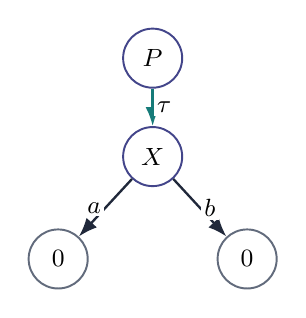
\begin{tikzpicture}[x=1cm,y=1cm]
        \node[st] (p) at (0,1.25) {$P$};
        \node[st] (x) at (0,0) {$X$};
        \node[terminal] (z1) at (-1.2,-1.3) {$0$};
        \node[terminal] (z2) at (1.2,-1.3) {$0$};
        \draw[tauedge] (p)--node[lab,right] {$\tau$}(x);
        \draw[trans] (x)--node[lab,left] {$a$}(z1);
        \draw[trans] (x)--node[lab,right] {$b$}(z2);
      \end{tikzpicture}
    \end{column}
    \begin{column}{.49\textwidth}\centering
      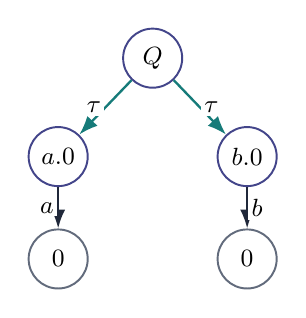
\begin{tikzpicture}[x=1cm,y=1cm]
        \node[st] (q) at (0,1.25) {$Q$};
        \node[st] (u) at (-1.2,0) {$a.0$};
        \node[st] (v) at (1.2,0) {$b.0$};
        \node[terminal] (z1) at (-1.2,-1.3) {$0$};
        \node[terminal] (z2) at (1.2,-1.3) {$0$};
        \draw[tauedge] (q)--node[lab,left] {$\tau$}(u);
        \draw[tauedge] (q)--node[lab,right] {$\tau$}(v);
        \draw[trans] (u)--node[lab,left] {$a$}(z1);
        \draw[trans] (v)--node[lab,right] {$b$}(z2);
      \end{tikzpicture}
    \end{column}
  \end{columns}
  \uncover<2->{\Takeaway{$P\notwb Q$: after $Q\step{\tau}a.0$, every possible silent response of $P$ still allows $b$.}}
  \note{Both P and X can perform b weakly. Neither can be related by a weak bisimulation to a.0. This also explains why the weak-bisimulation transfer clause must cover tau, not only visible labels.}
\end{frame}

% A3 ----------------------------------------------------------------
\begin{frame}{\optional Weak bisimilarity by saturation}
  \begin{block}{Saturated LTS}
    Keep the states and add an edge for every weak transition:
    \[
      p\step{\alpha}_{\mathrm{sat}}q
      \quad\Longleftrightarrow\quad
      p\wstep{\alpha}q
      \qquad(\alpha\in\Act).
    \]
    This includes \emph{all} $\tau^*$-shortcuts, not just $\tau$-self-loops.
  \end{block}
  \begin{block}{Characterisation}
    \[
      p\wb q\text{ in }T
      \quad\Longleftrightarrow\quad
      p\sim q\text{ in }T_{\mathrm{sat}}.
    \]
  \end{block}
  \Takeaway{Compute $\tau$-reachability, build the saturated graph, then reuse strong-bisimulation partition refinement.}
  \Source{Adapted and made explicit from the saturation idea in the supplied weak-bisimulation slides.}
\end{frame}

% A4 ----------------------------------------------------------------
\begin{frame}{\optional Why saturation works, and what it costs}
  \textbf{From weak to strong.} Repeatedly apply the weak transfer condition along the finite path
  \[
    \tau^*\,a\,\tau^*\quad\text{or}\quad\tau^*.
  \]
  Concatenating the responses gives a matching saturated edge with a related endpoint.
  \vspace{3mm}
  \textbf{From strong to weak.} Every original edge is a saturated edge; a matching saturated edge is exactly an allowed weak response.
  \begin{alertblock}{Finite-state cost}
    With $n$ states and $k=|\Act|$ labels, the saturated LTS can have up to $kn^2$ edges. The reduction can destroy sparsity. Include the cost of constructing saturation, not only of minimising it.
  \end{alertblock}
  \Source{This also proves that weak bisimilarity is an equivalence relation.}
\end{frame}

% A5 ----------------------------------------------------------------
\begin{frame}{\optional The precise divergence-preservation clause}
  Let $R$ be a symmetric branching bisimulation.
  \begin{block}{Explicit divergence condition}
    If $p\,R\,q$ and there is an infinite path
    \[
      p=p_0\step{\tau}p_1\step{\tau}p_2\cdots
      \quad\text{with }p_i\,R\,q\text{ for every }i,
    \]
    then there must be an infinite path
    \[
      q=q_0\step{\tau}q_1\step{\tau}q_2\cdots
      \quad\text{with }p_i\,R\,q_j\text{ for all }i,j.
    \]
  \end{block}
  We write $p\dbb q$ if some branching bisimulation satisfying this condition relates them.
  \Takeaway{The condition concerns divergence \emph{within related behaviour}; it is not merely an extra Boolean label saying ``can diverge''.}
  \Source{\cite[Section 3]{GLT09}; also \cite[Definition 2.1]{GLS20}.}
\end{frame}

% A6 ----------------------------------------------------------------
\begin{frame}{\optional The inertness proof in detail}
  Let $s\step{\tau}_T t$ and put $R=\Id\cup T\cup T^{-1}$.
  \par\vspace{2mm}
  \textbf{A move from $s$.} For $s\step{\alpha}u$, confluence gives
  \[
    t\optstep{\alpha}v,\qquad u=v\text{ or }u\step{\tau}_T v.
  \]
  The source pair is $(s,t)\in R$ and the target pair is $(u,v)\in R$.
  \par\vspace{2mm}
  \textbf{A move from $t$.} For $t\step{\alpha}v$, respond with
  \[
    s\step{\tau}_T t\step{\alpha}v.
  \]
  Use the identity pairs $(t,t)$ before the matching action and $(v,v)$ afterwards.
  \Takeaway{Identity and converse pairs give the remaining cases. Thus $R$ is a branching bisimulation.}
  \Source{Proof for the sufficient condition in \cite{GP00}.}
\end{frame}

% A7 ----------------------------------------------------------------
\begin{frame}{\optional Weak modal observations}
  Replace the one-step modality of Hennessy--Milner logic by a weak modality:
  \[
    \varphi::=\top\mid\neg\varphi\mid\varphi\land\varphi
       \mid\langle\!\langle\alpha\rangle\!\rangle\varphi,
       \qquad \alpha\in\Act,
  \]
  \[
    p\models\langle\!\langle\alpha\rangle\!\rangle\varphi
    \quad\Longleftrightarrow\quad
    \exists q:\ p\wstep{\alpha}q\ \land\ q\models\varphi.
  \]
  \begin{block}{Finite LTSs}
    Two states are weakly bisimilar iff they satisfy the same formulas of this logic.
  \end{block}
  \textbf{Reason:} apply the Hennessy--Milner theorem to the saturated LTS.
  \begin{alertblock}{Keep the $\tau$-modality}
    $a.\nil+\tau.\nil$ satisfies
    $\langle\!\langle\tau\rangle\!\rangle\neg\langle\!\langle a\rangle\!\rangle\top$,
    but $a.\nil$ does not.
  \end{alertblock}
  \note{This is an explicit deduction from saturation and the finite-state HML theorem from Lecture 3. It makes no unqualified claim about CTL preservation on arbitrary action-labelled LTSs.}
\end{frame}

\section{References}
% A8 ----------------------------------------------------------------
\begin{frame}{References: abstraction and congruence}
  \small
  \begin{thebibliography}{GLS20}
    \bibitem[GW96]{GW96}
      R. J. van Glabbeek and W. P. Weijland.
      \emph{Branching Time and Abstraction in Bisimulation Semantics}.
      Journal of the ACM 43(3), 555--600, 1996.
      \newblock\href{https://theory.stanford.edu/~rvg/abstraction/}{Author-hosted version}.
    \bibitem[GLT09]{GLT09}
      R. J. van Glabbeek, B. Luttik, and N. Tr\v{c}ka.
      \emph{Branching Bisimilarity with Explicit Divergence}.
      Fundamenta Informaticae 93(4), 371--392, 2009.
      \newblock\href{https://arxiv.org/abs/0812.3068}{arXiv:0812.3068}.
    \bibitem[GLS20]{GLS20}
      R. J. van Glabbeek, B. Luttik, and L. Spaninks.
      \emph{Rooted Divergence-Preserving Branching Bisimilarity is a Congruence}.
      Logical Methods in Computer Science 16(3:14), 2020.
      \newblock\href{https://arxiv.org/abs/1801.01180}{arXiv:1801.01180}.
  \end{thebibliography}
\end{frame}

% A9 ----------------------------------------------------------------
\begin{frame}{References: reduction and source material}
  \small
  \begin{thebibliography}{MCS}
    \bibitem[GP00]{GP00}
      J. F. Groote and J. van de Pol.
      \emph{State Space Reduction using Partial $\tau$-Confluence}.
      CWI report SEN-R0008, 2000, especially Sections 2 and 5.
      \newblock\href{https://ir.cwi.nl/pub/4446}{CWI repository record}.
    \bibitem[MCS]{MCS}
      R. J. van Glabbeek.
      \emph{Modelling Concurrent Systems: course notes}.
      University of Edinburgh, 2024, especially Lectures 6--8.
      \newblock\href{https://homepages.inf.ed.ac.uk/rvangla/MCS/notes.html}{Author's course notes}.
  \end{thebibliography}
  \begin{block}{Basis and additions}
    The supplied weak-bisimulation and process-algebra slides provide the starting material. Branching bisimulation, divergence, and rootedness are developed for this lecture. The former global CCS-confluence section is replaced by the local $\tau$-reduction criterion above.
  \end{block}
  \Source{A source map, corrections to the old slides, and teaching cautions are recorded in \texttt{lecture5\_notes.md}.}
\end{frame}

\end{document}
'
% Sources, scope changes, and technical cautions: lecture5_notes.md.
\ifdefined\HANDOUT
  \documentclass[handout,aspectratio=169,11pt]{beamer}
\else
  \documentclass[aspectratio=169,11pt]{beamer}
\fi
\usepackage[T1]{fontenc}
\usepackage[utf8]{inputenc}
\usepackage{lmodern}
\usepackage{amsmath,amssymb,mathtools,booktabs,array}
\usepackage{tikz}
\usetikzlibrary{arrows.meta,positioning,calc,fit,backgrounds}
\usepackage{appendixnumberbeamer}
\usefonttheme{professionalfonts}

\definecolor{Ink}{HTML}{20283A}
\definecolor{Indigo}{HTML}{43458A}
\definecolor{Pale}{HTML}{F0F0F8}
\definecolor{Teal}{HTML}{167B79}
\definecolor{PaleTeal}{HTML}{EAF5F3}
\definecolor{Warn}{HTML}{A4433C}
\definecolor{PaleWarn}{HTML}{FBF0EE}
\definecolor{Muted}{HTML}{626B7C}
\setbeamercolor{normal text}{fg=Ink,bg=white}
\setbeamercolor{structure}{fg=Indigo}
\setbeamercolor{frametitle}{fg=Indigo}
\setbeamercolor{title}{fg=Indigo}
\setbeamercolor{block title}{fg=Indigo,bg=Pale}
\setbeamercolor{block body}{fg=Ink,bg=Pale}
\setbeamercolor{block title example}{fg=Teal,bg=PaleTeal}
\setbeamercolor{block body example}{fg=Ink,bg=PaleTeal}
\setbeamercolor{block title alerted}{fg=Warn,bg=PaleWarn}
\setbeamercolor{block body alerted}{fg=Ink,bg=PaleWarn}
\setbeamertemplate{blocks}[rounded][shadow=false]
\setbeamertemplate{navigation symbols}{}
\setbeamertemplate{bibliography item}[text]
\pdfstringdefDisableCommands{\def\translate#1{#1}}
\setbeamersize{text margin left=8mm,text margin right=8mm}
\setbeamerfont{frametitle}{size=\Large,series=\bfseries}
\setbeamerfont{block title}{size=\normalsize,series=\bfseries}
\setbeamerfont{footnote}{size=\scriptsize}
\setbeamertemplate{itemize item}{\small\raise0.2ex\hbox{\textbullet}}
\setbeamertemplate{itemize subitem}{\tiny\raise0.2ex\hbox{\textbullet}}
\setbeamercovered{invisible}
\setbeameroption{hide notes}
\newif\ifinbackup
\inbackupfalse
\setbeamertemplate{headline}{\color{Indigo}\rule{\paperwidth}{0.5mm}}
\setbeamertemplate{footline}{%
  \leavevmode\hbox{%
    \begin{beamercolorbox}[wd=.79\paperwidth,ht=3.5mm,dp=2mm,leftskip=8mm]{normal text}%
      \color{Muted}\scriptsize Theory of Concurrency\enspace/\enspace Lecture 5\enspace/\enspace\insertsectionhead
    \end{beamercolorbox}%
    \begin{beamercolorbox}[wd=.21\paperwidth,ht=3.5mm,dp=2mm,rightskip=8mm plus1fil]{normal text}%
      \hfill\color{Muted}\scriptsize\ifinbackup Backup\enspace\fi\insertframenumber\,/\,\inserttotalframenumber
    \end{beamercolorbox}%
  }}
\setlength{\abovedisplayskip}{6pt}
\setlength{\belowdisplayskip}{6pt}
\newcommand{\step}[1]{\xrightarrow{#1}}
\newcommand{\wstep}[1]{\xRightarrow{#1}}
\newcommand{\silent}{\mathrel{\Rightarrow}}
\newcommand{\optstep}[1]{\xrightarrow{(#1)}}
\newcommand{\wb}{\mathrel{\approx_{\mathrm w}}}
\newcommand{\bb}{\mathrel{\approx_{\mathrm b}}}
\newcommand{\rbb}{\mathrel{\approx_{\mathrm{rb}}}}
\newcommand{\rwb}{\mathrel{\approx_{\mathrm{rw}}}}
\newcommand{\dbb}{\mathrel{\approx_{\mathrm b}^{\Delta}}}
\newcommand{\notwb}{\mathrel{\not\approx_{\mathrm w}}}
\newcommand{\notbb}{\mathrel{\not\approx_{\mathrm b}}}
\newcommand{\notrbb}{\mathrel{\not\approx_{\mathrm{rb}}}}
\newcommand{\notdbb}{\mathrel{\not\approx_{\mathrm b}^{\Delta}}}
\newcommand{\nil}{\mathbf 0}
\newcommand{\Act}{\Sigma_\tau}
\newcommand{\blockact}[2]{\operatorname{block}_{#1}(#2)}
\newcommand{\hide}[2]{\operatorname{hide}_{#1}(#2)}
\newcommand{\restr}[2]{(\nu #1)\,#2}
\newcommand{\Tr}{\operatorname{Tr}}
\newcommand{\CT}{\operatorname{CT}}
\newcommand{\Id}{\operatorname{Id}}
\newcommand{\Source}[1]{\par\vspace{2mm}{\scriptsize\color{Muted}#1\par}}
\newcommand{\Takeaway}[1]{\begin{exampleblock}{}#1\end{exampleblock}}
\newcommand{\optional}{\textcolor{Muted}{\scriptsize OPTIONAL}\quad}
\tikzset{
  >=Latex,
  st/.style={circle,draw=Indigo,line width=.7pt,fill=white,minimum size=7.5mm,inner sep=1pt,font=\small},
  terminal/.style={st,draw=Muted},
  trans/.style={->,line width=.85pt,draw=Ink},
  tauedge/.style={trans,draw=Teal},
  newedge/.style={trans,draw=Warn,line width=1.1pt},
  rel/.style={dashed,draw=Teal,line width=.85pt},
  lab/.style={font=\small,fill=white,inner sep=1.2pt},
  tinylabel/.style={font=\scriptsize,fill=white,inner sep=1pt},
  panel/.style={rounded corners=2mm,fill=Pale,draw=none,inner sep=4mm}
}
\title{Congruence and abstraction}
\subtitle{Lecture 5: Weak and branching bisimulation}
\author{Piotr Hofman}
\institute{Theory of Concurrency}
\date{}

\begin{document}

% 1 -----------------------------------------------------------------
\section{Overview}
\begin{frame}[plain]
  \vspace{8mm}
  {\color{Muted}\large THEORY OF CONCURRENCY\par}
  \vspace{6mm}
  {\color{Indigo}\LARGE\bfseries Congruence and abstraction\par}
  \vspace{3mm}
  {\Large From strong to weak and branching bisimulation\par}
  \vspace{7mm}
  {\large Lecture 5\quad\textcolor{Muted}{Piotr Hofman}\par}
  \vfill
  \begin{beamercolorbox}[sep=3mm,wd=\textwidth]{block body}
    First: when does equivalence support substitution?\\[1mm]
    Then: how much internal behaviour may an abstraction forget?
  \end{beamercolorbox}
  \vspace{3mm}
\end{frame}

% 2 -----------------------------------------------------------------


% 3 -----------------------------------------------------------------
\section{Congruence}
\begin{frame}{Congruence: equality compatible with operations}
  Let $\mathcal A$ be a set equipped with operations $f:\mathcal A^n\to\mathcal A$.
  \begin{block}{Definition}
    An equivalence relation $\equiv$ is a \textbf{congruence} if, for every operation $f$,
    \[
      x_i\equiv y_i\ (1\leq i\leq n)
      \quad\Longrightarrow\quad
      f(x_1,\ldots,x_n)\equiv f(y_1,\ldots,y_n).
    \]
  \end{block}
  \begin{exampleblock}{A familiar example: integers modulo $2$}
    If $x\equiv_2 x'$ and $y\equiv_2 y'$, then
    \[
      x+y\equiv_2 x'+y',\qquad xy\equiv_2 x'y'.
    \]
    Parity is a congruence for addition and multiplication.
  \end{exampleblock}
  \Takeaway{The requirement depends on the chosen operations, not only on the equivalence relation.}
  \Source{The general algebraic definition; process congruence is its application to system constructors.}
\end{frame}

% 4 -----------------------------------------------------------------
\begin{frame}{Why congruence gives a well-defined quotient}
  Every equivalence partitions $\mathcal A$ into classes $[x]$.
  We would like to define operations on classes by
  \[
    \overline f([x_1],\ldots,[x_n])=[f(x_1,\ldots,x_n)].
  \]
  \begin{block}{The role of congruence}
    The result must not depend on the representatives $x_1,\ldots,x_n$.
    This is \emph{exactly} the compatibility requirement in the definition.
  \end{block}
  \begin{exampleblock}{For systems}
    Build a larger system from the behavioural classes of its components,
    without inspecting which representatives were chosen.
  \end{exampleblock}
  \Takeaway{Congruence makes ``compute with behaviours instead of implementations'' mathematically meaningful.}
  \note{This is a quotient algebra of processes under constructors. It is distinct from the quotient of states inside a single LTS used for partition-refinement minimisation. Do not infer that an arbitrary state equivalence yields a behaviour-preserving quotient transition system.}
\end{frame}

% 5 -----------------------------------------------------------------
\section{Processes and contexts}
\begin{frame}{Processes and a small collection of operations}
  \begin{block}{For now: every action is visible}
    An LTS is $T=(S,\Sigma,\to)$, with ${\to}\subseteq S\times\Sigma\times S$.
    A process is an LTS with a distinguished state.
  \end{block}
  \renewcommand{\arraystretch}{1.4}
  \begin{tabular}{@{}p{.21\textwidth}p{.74\textwidth}@{}}
    $\nil$ & No outgoing transitions.\\
    $a.P$ & Perform $a\in\Sigma$, then behave as $P$.\\
    $P+Q$ & Perform a first transition of one summand; discard the other.\\
    $\blockact{H}{P}$ & Disable transitions labelled in $H\subseteq\Sigma$.
  \end{tabular}
  \vspace{2mm}
  \Takeaway{These are operations on LTSs; expressions are just convenient notation.}
  \Source{No acceptance predicate or successful-termination marker. Cyclic processes may be given directly as graphs.}
  \note{The initial fragment deliberately needs neither internal actions nor a full process calculus. Action blocking is written explicitly instead of using a channel-restriction shorthand. Later we add hiding and CCS parallel composition.}
\end{frame}




% 6 -----------------------------------------------------------------
\begin{frame}{The operations are defined by transition rules}
  \begin{block}{Prefix and choice}
    \[
      \frac{}{a.P\step{a}P}
      \qquad
      \frac{P\step{a}P'}{P+Q\step{a}P'}
      \qquad
      \frac{Q\step{a}Q'}{P+Q\step{a}Q'}.
    \]
  \end{block}
  \begin{block}{Blocking: restriction to allowed actions}
    \[
      \frac{P\step{a}P'}{\blockact{H}{P}\step{a}\blockact{H}{P'}}
      \qquad a\notin H.
    \]
    No rule permits an action in $H$.
  \end{block}
  \[
    a.b.\nil+a.c.\nil\step{a}b.\nil,
    \qquad \blockact{\{c\}}{c.\nil}\sim\nil.
  \]
  \Source{Prefix and choice follow the supplied CCS rules; blocking is the label-based restriction operation.}
\end{frame}

% 7 -----------------------------------------------------------------
\begin{frame}{Process congruence: replacement in every context}
  A finite \textbf{one-hole context} is built from the chosen operations:
  \[
    C[-]::=[-]\mid a.C[-]\mid C[-]+R\mid R+C[-]\mid\blockact{H}{C[-]}.
  \]
  Here $R$ is any fixed process. $C[P]$ is obtained by filling the hole with $P$.
  \begin{block}{Equivalent formulation of compatibility}
    \[
      P\equiv Q\quad\Longrightarrow\quad C[P]\equiv C[Q]
      \quad\text{for every allowed }C[-].
    \]
  \end{block}
  \begin{alertblock}{A different requirement from logical preservation}
    Satisfying the same formulas concerns \emph{observations}. Congruence concerns
    \emph{operations that build larger systems}.
  \end{alertblock}
  \Source{Adapted from the supplied context definitions; see also \cite{MCS}.}
  \note{Operator compatibility implies context compatibility by induction on the finite context. The converse follows by fixing all but one argument of an operation and replacing the arguments one at a time. No recursion-binding contexts are included.}
\end{frame}


\begin{frame}{Congruence: from basic operations to contexts}
  \begin{block}{Lemma}
    Let $\equiv$ be an equivalence relation on processes.
    The following conditions are equivalent:
    \begin{enumerate}
      \item $\equiv$ is compatible with every basic process operation.
      \item For every finite one-hole context $C[-]$ built from these
            operations and fixed processes,
            \[
              P\equiv Q \quad\Longrightarrow\quad C[P]\equiv C[Q].
            \]
    \end{enumerate}
  \end{block}

  \begin{block}{Proof sketch}
    \textbf{$(1)\Rightarrow(2)$.}
    Structural induction on $C[-]$: apply compatibility at each
    constructor and reflexivity for the fixed arguments.

    \medskip
    \textbf{$(2)\Rightarrow(1)$.}
    Fix all arguments of a basic operation except one.
    This gives a one-hole context, hence compatibility in that argument.
    Replace the arguments one at a time and use transitivity.
  \end{block}

 % \Takeaway{Compatibility with contexts is not an additional requirement: checking the basic operations suffices.}
\end{frame}

% 8 -----------------------------------------------------------------
\begin{frame}{Strong bisimilarity is a congruence}
  \begin{block}{Theorem for the operators just defined}
    \[
      P\sim Q\quad\Longrightarrow\quad C[P]\sim C[Q].
    \]
  \end{block}
  \textbf{Example: preservation by choice.} Assume $P\sim Q$ and fix $R$.
  \begin{itemize}\setlength\itemsep{3mm}
    \item A move of $P+R$ coming from $P$ is matched by a move of $Q$ with a bisimilar successor.
    \item A move coming from $R$ is matched by the identical move of $R$.
  \end{itemize}
  The same reasoning applies in the reverse direction.
  %\Takeaway{Prove compatibility with each constructor, then use induction on the context.}
  \Source{Compatibility for the displayed constructors; see \cite{MCS}.}
  \note{Explicit correction to old prezentacja(1).pdf, page 33: the printed claim 'not a congruence' contradicts its proof sketch and is false for these operators. At this point only prefix, choice and blocking are in scope. Prefix gives related successors; blocking filters the same labels on both sides. Compatibility with parallel and hiding will be used after those operations have been introduced.}
\end{frame}

% 9 -----------------------------------------------------------------
\section{Traces versus bisimulation}
\begin{frame}{Trace equivalence is also a congruence}
  Use the language of \textbf{all finite traces}, including the empty word:
  \[
    \Tr(P)=\{w\in\Sigma^*: P\step{w}P'\text{ for some }P'\}.
  \]
  \begin{block}{The trace language of a composite is determined by its operands}
    \[
    \begin{aligned}
      \Tr(\nil)&=\{\varepsilon\},\\
      \Tr(a.P)&=\{\varepsilon\}\cup a\Tr(P),\\
      \Tr(P+Q)&=\Tr(P)\cup\Tr(Q),\\
      \Tr(\blockact{H}{P})&=\Tr(P)\cap(\Sigma\setminus H)^*.
    \end{aligned}
    \]
  \end{block}
  \Takeaway{Congruence \emph{alone} does not justify choosing bisimulation over trace equivalence. We also need to specify what must be observed.}
  \note{This is the all-finite-traces convention, not an accepted language 
  with designated final states and not the 
  infinite-word semantics of LTL. Standard CCS 
  finite visible trace equivalence is also compositional, 
  but its extra operators are not needed for the argument here.}
\end{frame}




% 10 -----------------------------------------------------------------
\begin{frame}{The same traces, different choices after interaction}
  \[
    P=a.(b.\nil+c.\nil),\qquad Q=a.b.\nil+a.c.\nil.
  \]
  \begin{columns}[T,onlytextwidth]
    \begin{column}{.48\textwidth}\centering
      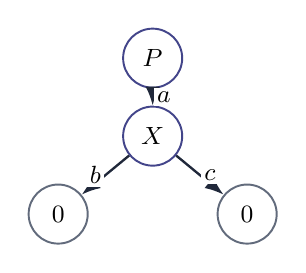
\begin{tikzpicture}[x=1cm,y=.9cm]
        \node[st] (p) at (0,1.1) {$P$}; \node[st] (x) at (0,0) {$X$};
        \node[terminal] (z1) at (-1.2,-1.1) {$0$}; \node[terminal] (z2) at (1.2,-1.1) {$0$};
        \draw[trans] (p)--node[lab,right] {$a$}(x);
        \draw[trans] (x)--node[lab,left] {$b$}(z1);
        \draw[trans] (x)--node[lab,right] {$c$}(z2);
      \end{tikzpicture}
    \end{column}
    \begin{column}{.48\textwidth}\centering
      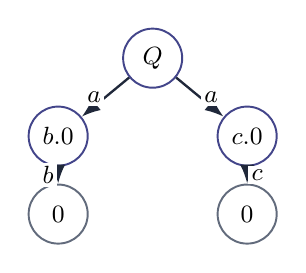
\begin{tikzpicture}[x=1cm,y=.9cm]
        \node[st] (q) at (0,1.1) {$Q$};
        \node[st] (u) at (-1.2,0) {$b.0$}; \node[st] (v) at (1.2,0) {$c.0$};
        \node[terminal] (z1) at (-1.2,-1.1) {$0$}; \node[terminal] (z2) at (1.2,-1.1) {$0$};
        \draw[trans] (q)--node[lab,left] {$a$}(u); \draw[trans] (q)--node[lab,right] {$a$}(v);
        \draw[trans] (u)--node[lab,left] {$b$}(z1); \draw[trans] (v)--node[lab,right] {$c$}(z2);
      \end{tikzpicture}
    \end{column}
  \end{columns}
  \[
    \Tr(P)=\Tr(Q)=\{\varepsilon,a,ab,ac\},\qquad P\not\sim Q.
  \]
  \Takeaway{$P$ satisfies $\langle a\rangle(\langle b\rangle\top\land\langle c\rangle\top)$; $Q$ does not.}
\end{frame}




% 11 -----------------------------------------------------------------
\begin{frame}{Deadlock observations can destroy congruence}
  A \textbf{finite completed trace} ends in a deadlock:
  \[
    \CT(P)=\{w:P\step{w}P'\text{ and }P'\text{ has no outgoing transition}\}.
  \]
  For the preceding $P$ and $Q$, $\CT(P)=\CT(Q)=\{ab,ac\}$.
  \begin{alertblock}{An environment that blocks $c$}
    \[
    \begin{aligned}
      \CT(\blockact{\{c\}}{P})&=\{ab\},\\
      \CT(\blockact{\{c\}}{Q})&=\{a,ab\}.
    \end{aligned}
    \]
    The second process can commit to its $c$-branch and become stuck after $a$.
  \end{alertblock}
  \Takeaway{The ordinary trace languages still agree. Completed-trace equality is not a congruence for blocking.}
  \note{For general infinite-state systems, completed-trace equivalence is often defined to preserve both all traces and completed traces. This example refutes congruence under either convention: the original pair agrees on both. All displayed processes are finite and have no successful-termination predicate.}
\end{frame}

% 12 -----------------------------------------------------------------
\begin{frame}{Why make bisimulation our baseline?}
  \begin{block}{The verification objective}
    Preserve the available continuations after every matched interaction,
    including branching observations and deadlock behaviour.
  \end{block}
  \renewcommand{\arraystretch}{1.45}
  \begin{tabular}{@{}p{.26\textwidth}p{.68\textwidth}@{}}
    \textbf{Logical} & Strong bisimulation preserves HML; on Kripke structures, its label-preserving version preserves CTL$^*$.\\
    \textbf{Algebraic} & It supports substitution under the chosen constructors.\\
    \textbf{Proof-theoretic} & A witness is checked locally by matching transitions; finite-state minimisation uses partition refinement.
  \end{tabular}
  \vspace{2mm}
  \note{Do not say that traces cannot express liveness: 
  equality of infinite state-labelled trace languages preserves LTL, 
  including LTL liveness. 
  Nor do deadlock and compositionality alone uniquely characterise bisimulation: 
  failure/testing semantics offers intermediate alternatives. 
  The chosen baseline reflects this course's branching-time analysis and local proof methods.}
\end{frame}

% 13 -----------------------------------------------------------------
\section{Internal actions and abstraction}
\begin{frame}{Now add internal actions and abstraction}
  Let $\Act=\Sigma\cup\{\tau\}$, with $\tau\notin\Sigma$.\\[1mm]
  $a,b,c\in\Sigma$ are visible; $\alpha\in\Act$ may be internal.\par\vspace{2mm}
  \centering
  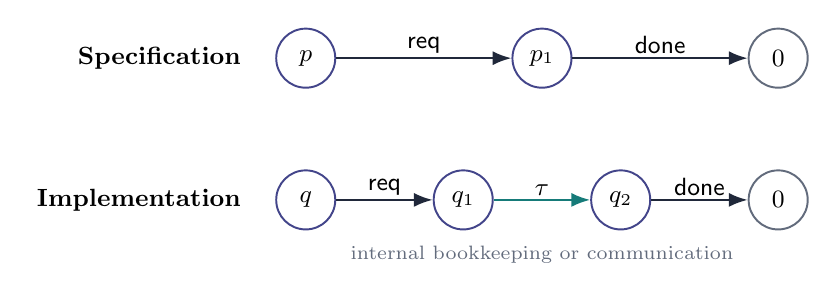
\begin{tikzpicture}[x=1cm,y=1cm]
    \node[anchor=east,font=\small\bfseries] at (-.7,1.35) {Specification};
    \node[st] (p) at (0,1.35) {$p$};
    \node[st] (p1) at (3,1.35) {$p_1$};
    \node[terminal] (p2) at (6,1.35) {$0$};
    \draw[trans] (p)--node[lab,above] {$\mathsf{req}$}(p1);
    \draw[trans] (p1)--node[lab,above] {$\mathsf{done}$}(p2);
    \node[anchor=east,font=\small\bfseries] at (-.7,-.45) {Implementation};
    \node[st] (q) at (0,-.45) {$q$};
    \node[st] (q1) at (2,-.45) {$q_1$};
    \node[st] (q2) at (4,-.45) {$q_2$};
    \node[terminal] (q3) at (6,-.45) {$0$};
    \draw[trans] (q)--node[lab,above] {$\mathsf{req}$}(q1);
    \draw[tauedge] (q1)--node[lab,above] {$\tau$}(q2);
    \draw[trans] (q2)--node[lab,above] {$\mathsf{done}$}(q3);
    \node[font=\scriptsize,text=Muted] at (3,-1.15) {internal bookkeeping or communication};
  \end{tikzpicture}
  \par\vspace{2mm}
  \begin{block}{External behaviour}
    Strong bisimulation distinguishes the initial states because of the internal step.
    We seek a coarser relation that can abstract from this bookkeeping.
  \end{block}
  \note{Spoiler performs req and then the implementation's tau. The specification cannot match that tau strongly. Do not identify hiding with edge deletion: hiding changes labels, retaining the intermediate states and alternatives.}
\end{frame}

% 14 -----------------------------------------------------------------
\begin{frame}{The simplified process algebra with internal actions}
  Let $\Sigma$ contain the visible actions, with $\tau\notin\Sigma$.
  Write
  \[
    \Sigma_\tau=\Sigma\cup\{\tau\},
    \qquad \alpha\in\Sigma_\tau,
    \qquad H\subseteq\Sigma.
  \]

  \begin{block}{Process constructors}
    \renewcommand{\arraystretch}{1.4}
    \begin{tabular}{@{}p{.25\textwidth}p{.69\textwidth}@{}}
      $\nil$
        & No outgoing transitions, not even internal ones.\\
      $\alpha.P$
        & Perform $\alpha$, then behave as $P$.
          In particular, $\tau.P\step{\tau}P$.\\
      $P+Q$
        & The first transition of either summand selects that
          summand and discards the other, even if its label is $\tau$.\\
      $\blockact{H}{P}$
        & Remove transitions labelled in $H$.
          Other transitions, including $\tau$-transitions, remain.\\
      $\hide{H}{P}$ \alert{(new)}
        & Replace labels in $H$ by $\tau$.
          Retain all states and transitions; leave other labels unchanged.


        \end{tabular}
  \end{block}


\end{frame}


\begin{frame}{The simplified process algebra with internal actions}
  Let $\Sigma$ contain the visible actions, with $\tau\notin\Sigma$.
  Write
  \[
    \Sigma_\tau=\Sigma\cup\{\tau\},
    \qquad \alpha\in\Sigma_\tau,
    \qquad H\subseteq\Sigma.
  \]


  \begin{exampleblock}{Blocking prevents an action; hiding conceals it}
    \[
      \blockact{\{a\}}{a.b.\nil}\sim\nil,
      \qquad
      \hide{\{a\}}{a.b.\nil}\sim\tau.b.\nil.
    \]
    After hiding $a$, the process can still reach and perform $b$.
  \end{exampleblock}
\end{frame}



\begin{frame}{Operational rules: an internal step is still a step}
  Throughout, $\alpha\in\Sigma_\tau$ and $H\subseteq\Sigma$.
  The process $\nil$ has no transition rules.

  \begin{block}{Prefix and choice: the same rules for visible and internal actions}
    \[
      \frac{}{\alpha.P\step{\alpha}P}
      \qquad
      \frac{P\step{\alpha}P'}{P+Q\step{\alpha}P'}
      \qquad
      \frac{Q\step{\alpha}Q'}{P+Q\step{\alpha}Q'}.
    \]
  \end{block}

  \begin{block}{Blocking and hiding}
    \[
      \frac{P\step{\alpha}P'}
           {\blockact{H}{P}\step{\alpha}\blockact{H}{P'}}
      \;(\alpha\notin H)
      \qquad
      \frac{P\step{\alpha}P'}
           {\hide{H}{P}\step{h_H(\alpha)}\hide{H}{P'}},
    \]
    where
    \[
      h_H(\alpha)=
      \begin{cases}
        \tau,   & \alpha\in H,\\
        \alpha, & \alpha\notin H.
      \end{cases}
      \qquad\text{In particular, }h_H(\tau)=\tau.
    \]
  \end{block}

\end{frame}



\begin{frame}{Operational rules: an internal step is still a step}
 

  \begin{alertblock}{A silent transition can resolve a choice}
    \[
      \tau.a.\nil+b.\nil\step{\tau}a.\nil,
      \qquad
      \tau.a.\nil+b.\nil\step{b}\nil.
    \]
    Both initial transitions are possible: $\tau$ has no priority.
    If the $\tau$-step occurs, the successor is $a.\nil$,
    \textbf{not} $a.\nil+b.\nil$: the $b$-alternative disappears.
  \end{alertblock}
\end{frame}

% 15 -----------------------------------------------------------------
\begin{frame}{A tempting but inadequate proposal: ignore silent moves}
  Suppose we compare only visible behaviour, allowing internal work before and after it,
  but impose \emph{no obligation} on a purely internal move.
  \[
    P=a.\nil+\tau.\nil,\qquad Q=a.\nil.
  \]
  \centering
  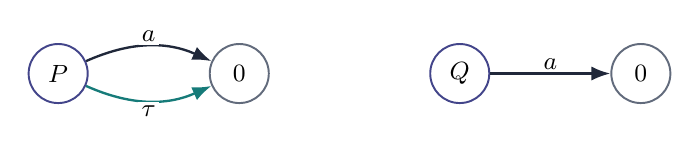
\begin{tikzpicture}[x=1cm,y=1cm]
    \node[st] (p) at (0,0) {$P$}; \node[terminal] (z) at (2.3,0) {$0$};
    \node[st] (q) at (5.1,0) {$Q$}; \node[terminal] (z2) at (7.4,0) {$0$};
    \draw[trans] (p) to[bend left=24] node[lab,above] {$a$}(z);
    \draw[tauedge] (p) to[bend right=24] node[lab,below] {$\tau$}(z);
    \draw[trans] (q)--node[lab,above] {$a$}(z2);
  \end{tikzpicture}
  \par\vspace{3mm}
  \begin{alertblock}{The silent-deadlock problem}
    Both can perform $a$, but only $P$ can silently become stuck \emph{before} $a$.
    The naive proposal ignores that commitment.
  \end{alertblock}
  \Takeaway{Internal transitions must also be matched, even when the matching response may do nothing.}
  \note{A precise failed definition uses the weak-transfer obligation only for visible labels. The symmetric relation {(P,Q),(Q,P),(0,0)} passes that test. This is deliberately not presented as weak bisimulation; the next definition adds the missing obligation. Contracting all internal edges is likewise unsound.}
\end{frame}

% 16 -----------------------------------------------------------------
\section{Weak bisimulation}
\begin{frame}{Weak transitions}
  \begin{block}{Zero or more internal steps}
    \[
      p\silent q\quad\Longleftrightarrow\quad p\step{\tau *}q.
    \]
    In particular, $p\silent p$ always holds.
  \end{block}
  \begin{block}{One visible action, with internal work around it}
    For $a\in\Sigma$,
    \[
      p\wstep{a}q\quad\Longleftrightarrow\quad
      \exists u,v:\ p\silent u\step{a}v\silent q.
    \]
    For uniform notation, define $\;p\wstep{\tau}q\;\Longleftrightarrow\;p\silent q$.
  \end{block}
  \Takeaway{A weak visible move contains exactly one visible action. A weak $\tau$-move may be empty. All matching paths are finite.}
  \Source{Weak-bisimulation notation adapted from the supplied slides; see also \cite{GW96}.}
\end{frame}

% 17 -----------------------------------------------------------------
\begin{frame}{Weak bisimulation}
  \begin{block}{Definition}
    A \textbf{symmetric} relation $R\subseteq S\times S$ is a weak bisimulation if
    \[
      p\,R\,q\ \land\ p\step{\alpha}p'
      \quad\Longrightarrow\quad
      \exists q':\ q\wstep{\alpha}q'\ \land\ p'\,R\,q'
      \qquad(\alpha\in\Act).
    \]
    We write $p\wb q$ if some weak bisimulation relates $p$ and $q$.
  \end{block}
  \centering
  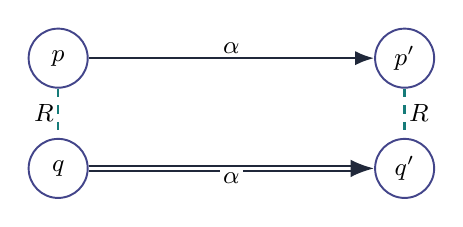
\begin{tikzpicture}[x=1cm,y=1cm]
    \node[st] (p) at (0,1.0) {$p$}; \node[st] (p1) at (4.4,1.0) {$p'$};
    \node[st] (q) at (0,-.4) {$q$}; \node[st] (q1) at (4.4,-.4) {$q'$};
    \draw[trans] (p)--node[lab,above] {$\alpha$}(p1);
    \draw[trans,double,double distance=1pt] (q)--node[lab,below] {$\alpha$}(q1);
    \draw[rel] (p)--node[lab,left] {$R$}(q);
    \draw[rel] (p1)--node[lab,right] {$R$}(q1);
  \end{tikzpicture}
  \par\vspace{1mm}
  {\small Symmetry supplies the same obligation for moves from $q$.}
  \Source{Weak bisimilarity is the greatest weak bisimulation and is an equivalence relation.}
  \note{The union of weak bisimulations is a weak bisimulation. The largest relation is weak bisimilarity and is an equivalence. These facts also follow from the saturation construction in the backup slides.}
\end{frame}


% ----------------------------------------------------------------------
\begin{frame}{Weak Hennessy--Milner logic}
  Recall
  \[
    p\Rightarrow q
    \quad\Longleftrightarrow\quad
    p\step{\tau *}q,
  \]
  and, for $a\in\Sigma$,
  \[
    p\xRightarrow{a}q
    \quad\Longleftrightarrow\quad
    p\step{\tau *}\step{a}\step{\tau *}q.
  \]

  \begin{block}{Weak modalities}
    \[
      \varphi ::= \top
      \mid \neg\varphi
      \mid \varphi\land\psi
      \mid \langle\!\langle\alpha\rangle\!\rangle\varphi,
      \qquad \alpha\in\Sigma\cup\{\tau\}.
    \]
    \[
      p\models\langle\!\langle\alpha\rangle\!\rangle\varphi
      \quad\Longleftrightarrow\quad
      \exists q:\;
      p\xRightarrow{\alpha}q
      \land q\models\varphi .
    \]
    For $\alpha=\tau$, we put $\xRightarrow{\tau}=\Rightarrow$,
    so zero or more internal steps are allowed.
  \end{block}

  \Takeaway{The logic observes the endpoint of a weak transition,
  but not the states crossed by its internal part.}
\end{frame}


% ----------------------------------------------------------------------
\begin{frame}{Weak HML characterizes weak bisimulation}
  \begin{block}{Theorem}
    For finite LTSs,
    \[
      p\approx_{\mathrm w}q
      \quad\Longleftrightarrow\quad
      \forall\varphi\in\mathrm{WHML}:
      \bigl(p\models\varphi\iff q\models\varphi\bigr).
    \]
  \end{block}



  \begin{block}{Why? Saturate the transition system}
    Construct $\mathrm{Sat}(T)$ by putting
    \[
      p\step{a}_{\mathrm w}q
      \quad\Longleftrightarrow\quad
      p\xRightarrow{a}q,  \text{ and }
    \]
    \[
      p\step{\tau}_{\mathrm w}q
      \quad\Longleftrightarrow\quad
      p\Rightarrow q.
    \]
    Then
    \[
      p\approx_{\mathrm w}q\text{ in }T
      \quad\Longleftrightarrow\quad
      p\sim q\text{ in }\mathrm{Sat}(T).
    \]
    Apply the ordinary Hennessy--Milner theorem to $\mathrm{Sat}(T)$.
  \end{block}

  \Takeaway{Weak bisimulation is ordinary bisimulation after forgetting
  the internal structure of finite silent computations.}
  \Source{Hennessy--Milner; De Nicola--Vaandrager.}
\end{frame}


% ----------------------------------------------------------------------
\begin{frame}{What if the logic can inspect a silent computation?}
  Weak HML sees only
  \[
      p \xRightarrow{a} q.
  \]
  It cannot ask what remains possible \emph{while} the silent preparation
  for $a$ is taking place.

  \begin{block}{A CTL-style ``until'' operator}
    Introduce
    \[
      \varphi\langle a\rangle\psi
    \]
    with the semantics
    \[
    p\models\varphi\langle a\rangle\psi
    \]
    iff there exist
    \[
      p=p_0\step{\tau}p_1\step{\tau}\cdots
      \step{\tau}p_n\step{a}q
    \]
    such that
    \[
      p_i\models\varphi\quad(0\leq i\leq n),
      \qquad q\models\psi.
    \]
  \end{block}

  \Takeaway{This is an ``until $a$ happens'' modality:
  it observes properties of the intermediate silent states.}

  \note{This is the essential operator of Hennessy--Milner Logic with Until,
  HMLU. I would call it CTL-style rather than ``weak CTL'', because
  ``CTL over the saturated LTS'' would have different semantics.}
\end{frame}


% ----------------------------------------------------------------------
\begin{frame}{Until can distinguish weakly bisimilar processes}
  Consider
  \[
    R=\tau.a.\nil+b.\nil,
    \qquad
    S=a.\nil+\tau.a.\nil+b.\nil.
  \]

  \begin{columns}[T,onlytextwidth]
    \begin{column}{.46\textwidth}\centering
      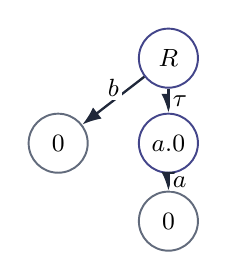
\begin{tikzpicture}[x=1cm,y=.9cm]
        \node[st] (r) at (0,1.2) {$R$};
        \node[st] (r1) at (0,0) {$a.0$};
        \node[terminal] (z1) at (0,-1.1) {$0$};
        \node[terminal] (z2) at (-1.4,0) {$0$};

        \draw[trans] (r)--node[lab,right] {$\tau$}(r1);
        \draw[trans] (r1)--node[lab,right] {$a$}(z1);
        \draw[trans] (r)--node[lab,above] {$b$}(z2);
      \end{tikzpicture}
    \end{column}

    \begin{column}{.50\textwidth}\centering
      \begin{tikzpicture}[x=1cm,y=.9cm]
        \node[st] (s) at (0,1.2) {$S$};
        \node[st] (s1) at (0,0) {$a.0$};
        \node[terminal] (za) at (1.4,0) {$0$};
        \node[terminal] (zb) at (-1.4,0) {$0$};
        \node[terminal] (z1) at (0,-1.1) {$0$};

        \draw[trans] (s)--node[lab,right] {$\tau$}(s1);
        \draw[trans] (s1)--node[lab,right] {$a$}(z1);
        \draw[trans] (s)--node[lab,above] {$a$}(za);
        \draw[trans] (s)--node[lab,above] {$b$}(zb);
      \end{tikzpicture}
    \end{column}
  \end{columns}

  \[
      R\approx_{\mathrm w}S.
  \]

  But let
  \[
      \chi=
      \bigl(\langle\!\langle b\rangle\!\rangle\top\bigr)
      \langle a\rangle\top.
  \]
  Then
  \[
      S\models\chi,
      \qquad
      R\not\models\chi.
  \]

  \Takeaway{Weak bisimulation forgets too much for an until operator
  that inspects the internal path.}
\end{frame}


% ----------------------------------------------------------------------
\begin{frame}{What exactly does the formula observe?}
  \[
      \chi=
      \bigl(\langle\!\langle b\rangle\!\rangle\top\bigr)
      \langle a\rangle\top.
  \]

  \begin{block}{$S\models\chi$}
    $S$ may perform $a$ immediately:
    \[
       S\step{a}0.
    \]
    Before $a$ happens, we are still in $S$, where $b$ is possible.
  \end{block}

  \begin{alertblock}{$R\not\models\chi$}
    Every execution of $a$ has to start with
    \[
       R\step{\tau}a.0\step{a}0.
    \]
    After the silent step the $b$-alternative has disappeared:
    \[
       a.0\not\models
       \langle\!\langle b\rangle\!\rangle\top.
    \]
  \end{alertblock}

  \Takeaway{The difference is not the visible trace.
  It is \emph{when a branching possibility disappears}.}
\end{frame}


% ----------------------------------------------------------------------
\begin{frame}{Branching bisimulation}
  \begin{block}{Definition}
    A symmetric relation $R$ is a \textbf{branching bisimulation} if
    $p\,R\,q$ and
    \[
       p\step{\alpha}p'
    \]
    imply either
    \[
       \alpha=\tau
       \quad\text{and}\quad p'\,R\,q,
    \]
    or there exist $q_0,q'$ such that
    \[
       q\Rightarrow q_0\step{\alpha}q',
       \qquad
       p\,R\,q_0,
       \qquad
       p'\,R\,q'.
    \]
  \end{block}

  \begin{center}
    \begin{tikzpicture}[x=1.25cm,y=.9cm]
      \node[st] (p)  at (0,1) {$p$};
      \node[st] (pp) at (4,1) {$p'$};
      \node[st] (q)  at (0,-.5) {$q$};
      \node[st] (q0) at (2,-.5) {$q_0$};
      \node[st] (qp) at (4,-.5) {$q'$};

      \draw[trans] (p)--node[lab,above] {$\alpha$}(pp);
      \draw[trans,double,double distance=1pt]
         (q)--node[lab,below] {$\tau^*$}(q0);
      \draw[trans] (q0)--node[lab,below] {$\alpha$}(qp);
      \draw[rel] (p)--node[lab,left] {$R$}(q);
      \draw[rel] (p)--node[lab,right] {$R$}(q0);
      \draw[rel] (pp)--node[lab,right] {$R$}(qp);
    \end{tikzpicture}
  \end{center}

  \Takeaway{Silent preparation may be ignored only while the original
  branching situation is preserved.}
\end{frame}


% ----------------------------------------------------------------------
\begin{frame}{Weak versus branching bisimulation}
  For the previous processes,
  \[
      R=\tau.a.0+b.0,
      \qquad
      S=a.0+\tau.a.0+b.0,
  \]
  we have
  \[
      R\approx_{\mathrm w}S,
      \qquad
      R\not\approx_{\mathrm b}S.
  \]

  \begin{block}{Why does branching bisimulation fail?}
    Consider the direct transition
    \[
       S\step{a}0.
    \]
    The only way $R$ can prepare an $a$ is
    \[
       R\step{\tau}a.0\step{a}0.
    \]
    Branching bisimulation would require
    \[
       S\approx_{\mathrm b}a.0
    \]
    immediately before the matching $a$.
    This is impossible: $S$ still offers $b$, while $a.0$ does not.
  \end{block}

  \Takeaway{Branching bisimulation remembers which choices survive
  during an internal computation.}
\end{frame}


% ----------------------------------------------------------------------
\begin{frame}{Hennessy--Milner logic with Until}
  \begin{block}{HMLU}
    \[
      \varphi ::=
      \top
      \mid\neg\varphi
      \mid\varphi\land\psi
      \mid\varphi\langle\alpha\rangle\psi .
    \]
    The last operator requires an internal path
    \[
      p=p_0\step{\tau}\cdots\step{\tau}p_n
      \step{\alpha}q
    \]
    such that every $p_i$ satisfies $\varphi$ and $q$ satisfies $\psi$.
  \end{block}

  \begin{block}{Theorem}
    For finite LTSs,
    \[
       p\approx_{\mathrm b}q
       \quad\Longleftrightarrow\quad
       p\text{ and }q\text{ satisfy the same HMLU formulas}.
    \]
  \end{block}

  \[
      \underbrace{\text{weak HML}}_{\text{endpoint only}}
      \quad\leadsto\quad
      \approx_{\mathrm w}
      \qquad
      \underbrace{\text{HMLU}}_{\text{inspect silent prefix}}
      \quad\leadsto\quad
      \approx_{\mathrm b}.
  \]

  \Takeaway{The extra logical power of ``until'' corresponds exactly
  to preservation of branching during silent computation.}
  \Source{De Nicola and Vaandrager, JACM 42(2), 1995.}
\end{frame}


% ----------------------------------------------------------------------
\begin{frame}{Connection with CTL without the next operator}
  HMLU already gives the cleanest action-based characterization.
  There is also a direct connection with CTL.

  \begin{block}{Translate an LTS to a state-labelled system}
    Keep original states and label them by a fresh proposition $\bot$.
    Replace every visible transition
    \[
        p\step{a}q
    \]
    by
    \[
        p\longrightarrow [p,a,q]\longrightarrow q,
    \]
    where the intermediate state is labelled by $a$.
    Silent transitions $p\step{\tau}q$ remain direct edges.
  \end{block}

  \begin{block}{Theorem for finite LTSs}
    Under the divergence-blind interpretation,
    \[
      p\approx_{\mathrm b}q
      \quad\Longleftrightarrow\quad
      p,q\text{ satisfy the same }\mathrm{CTL}^{*}\!-\!X
      \text{ formulas}.
    \]
    In fact, $\mathrm{CTL}-X$ already induces the same equivalence.
  \end{block}

  \Takeaway{Removing $X$ makes finite stuttering invisible,
  while Until still observes whether properties remain true
  throughout the stuttering segment.}
\end{frame}


% ----------------------------------------------------------------------
\begin{frame}{Infinite silence is a separate question}
  Consider
  \[
  \begin{array}{c@{\qquad\qquad}c}
    p\step{a}0
    &
    q\step{a}0,\qquad q\step{\tau}q .
  \end{array}
  \]

  \begin{block}{Ordinary weak and branching bisimulation}
    \[
       p\approx_{\mathrm w}q,
       \qquad
       p\approx_{\mathrm b}q.
    \]
    The $\tau$-loop can be ignored forever.
  \end{block}

  \begin{alertblock}{But there is an observable design question}
    $q$ admits an infinite internal computation
    \[
       q\step{\tau}q\step{\tau}q\step{\tau}\cdots,
    \]
    while $p$ does not.
  \end{alertblock}

  If this distinction matters, use a
  \textbf{divergence-preserving} version of the equivalence
  (and a corresponding divergence-sensitive logic).

  \Takeaway{Two independent questions arise:
  what may finite silent computation forget, and whether infinite silence matters.}
\end{frame}


% ----------------------------------------------------------------------
\begin{frame}{Weak and branching bisimilarity are not congruences}
  Both equivalences abstract from an initial finite silent computation:
  \[
       \tau.0\approx_{\mathrm w}0,
       \qquad
       \tau.0\approx_{\mathrm b}0.
  \]

  Now put the processes in the choice context
  \[
       C[-]=a.0+[-].
  \]

  Then
  \[
      C[\tau.0]=a.0+\tau.0,
      \qquad
      C[0]=a.0+0.
  \]

  But
  \[
      a.0+\tau.0\not\approx_{\mathrm w}a.0+0.
  \]
  The left process can silently choose the second branch and deadlock,
  while the right process cannot.

  Hence also
  \[
      a.0+\tau.0\not\approx_{\mathrm b}a.0+0.
  \]

  \Takeaway{The problem is at the root:
  an initial silent step may resolve an external choice.}
\end{frame}


% ----------------------------------------------------------------------
\begin{frame}{Rooted weak bisimilarity}
  To recover substitution under choice, treat the first move more strictly.

  Define
  \[
  q\xRightarrow{\widehat{\alpha}}q'=
  \begin{cases}
    q\Rightarrow\step{a}\Rightarrow q',
       & \alpha=a\in\Sigma,\\[1mm]
    q\Rightarrow\step{\tau}\Rightarrow q',
       & \alpha=\tau.
  \end{cases}
  \]
  Notice that a root $\tau$ must now be matched by
  \textbf{at least one} $\tau$.

  \begin{block}{Rooted weak bisimilarity}
    \[
      p\approx_{\mathrm{rw}}q
    \]
    iff every initial
    \[
      p\step{\alpha}p'
    \]
    can be matched by
    \[
      q\xRightarrow{\widehat{\alpha}}q'
      \qquad\text{with}\qquad
      p'\approx_{\mathrm w}q',
    \]
    and symmetrically.
  \end{block}

  Thus
  \[
     \tau.0\not\approx_{\mathrm{rw}}0.
  \]

  \Takeaway{After the root has been matched, ordinary weak
  bisimilarity is sufficient again.}
\end{frame}


% ----------------------------------------------------------------------
\begin{frame}{Rooted branching bisimilarity}
  For branching bisimulation the standard root condition is even cleaner.

  \begin{block}{Definition}
    \[
       p\approx_{\mathrm{rb}}q
    \]
    iff every initial transition
    \[
       p\step{\alpha}p'
    \]
    can be matched by an actual transition
    \[
       q\step{\alpha}q'
    \]
    such that
    \[
       p'\approx_{\mathrm b}q',
    \]
    and symmetrically.
  \end{block}

  \begin{block}{Compositional role}
    The rooted variants repair the failure under nondeterministic choice.
    For the standard CCS-style operators they give the corresponding
    congruences.
  \end{block}

  \Takeaway{Rootedness and branching preservation solve different problems:
  branching controls what may happen \emph{inside} a silent computation;
  rootedness controls how a component may be used by its environment.}
\end{frame}


% ----------------------------------------------------------------------
\begin{frame}{What $\tau$ adds to the picture}
  \begin{center}
  \renewcommand{\arraystretch}{1.45}
  \begin{tabular}{@{}lll@{}}
    \textbf{Observation} &
    \textbf{Logic} &
    \textbf{Equivalence}\\
    \hline
    every transition &
    HML &
    strong bisimulation\\

    endpoints of silent computations &
    weak HML &
    weak bisimulation\\

    branching preserved during silence &
    HML with Until &
    branching bisimulation\\

    finite stuttering in branching time &
    CTL$^{*}{-}X$ &
    branching bisimulation\\
  \end{tabular}
  \end{center}

  \vspace{4mm}

  Two additional refinements answer independent questions:
  \[
      \text{divergence preservation}
      \qquad\text{and}\qquad
      \text{rootedness / congruence}.
  \]

  \Takeaway{There is no single way to ``ignore $\tau$'':
  the equivalence depends on what the observer is allowed to see.}
\end{frame}

% 18 -----------------------------------------------------------------
\begin{frame}{First example: an internal delay}
  \[
    P=a.\nil,\qquad Q=\tau.a.\nil.
  \]
  \centering
  \begin{tikzpicture}[x=1cm,y=1cm]
    \node[st] (p) at (0,1.05) {$P$}; \node[terminal] (p0) at (5,1.05) {$0$};
    \node[st] (q) at (0,-.6) {$Q$}; \node[st] (q1) at (2.5,-.6) {$a.0$};
    \node[terminal] (q0) at (5,-.6) {$0$};
    \draw[trans] (p)--node[lab,above] {$a$}(p0);
    \draw[tauedge] (q)--node[lab,below] {$\tau$}(q1);
    \draw[trans] (q1)--node[lab,below] {$a$}(q0);
    \draw[rel] (p)--(q); \draw[rel] (p)--(q1); \draw[rel] (p0)--(q0);
  \end{tikzpicture}
  \par\vspace{1mm}
  \uncover<2->{\Takeaway{$P\wb Q$, but $P\not\sim Q$. The $\tau$-step of $Q$ can be matched by $P$ doing nothing.}}
  \note{The two displayed states named a.0/P have identical behaviour; the dotted links show a possible witness across disjoint copies. All displayed zero states are deadlocks.}
\end{frame}

% 19 -----------------------------------------------------------------
\begin{frame}{Weak bisimulation detects silent deadlock}
  Return to $P=a.\nil+\tau.\nil$ and $Q=a.\nil$.
  \begin{block}{The missing obligation is now present}
    If $P\,R\,Q$ and $P\step{\tau}\nil$, we need
    \[
      Q\silent Q'\quad\text{and}\quad\nil\,R\,Q'.
    \]
    $Q$ has no internal move, so $Q'=Q$.
    But $Q$ can perform $a$, and $\nil$ cannot match it.
  \end{block}
  Therefore $P\notwb Q$.
  \begin{exampleblock}{What is intentionally ignored}
    $\tau.\nil\wb\nil$: finite internal work leading only to inaction adds no visible possibility.

  \end{exampleblock}
  \Takeaway{Ignore the duration of finite internal work, not its effect on the available continuations.}
\end{frame}

% 20 -----------------------------------------------------------------
\section{Branching bisimulation}
\begin{frame}{Weak matching may pass over a choice}
  \centering
  \begin{tikzpicture}[x=1cm,y=1cm]
    \node[st] (p) at (0,1.3) {$p$}; \node[st] (pp) at (7,1.3) {$p'$};
    \node[st] (q) at (0,-.5) {$q$}; \node[st] (q0) at (2.3,-.5) {$q_0$};
    \node[st] (q1) at (4.7,-.5) {$q_1$}; \node[st] (qq) at (7,-.5) {$q'$};
    \draw[trans] (p)--node[lab,above] {$a$}(pp);
    \draw[tauedge] (q)--node[lab,below] {$\tau^*$}(q0);
    \draw[trans] (q0)--node[lab,below] {$a$}(q1);
    \draw[tauedge] (q1)--node[lab,below] {$\tau^*$}(qq);
    \draw[rel] (p)--node[lab,left] {$R$}(q);
    \draw[rel] (pp)--node[lab,right] {$R$}(qq);
    \uncover<2->{\draw[rel,line width=1.2pt] (p)--node[lab,above right] {$R$}(q0);
      \draw[rel,line width=1.2pt] (pp)--node[lab,above left] {$R$}(q1);}
  \end{tikzpicture}
  \par\vspace{4mm}
  \begin{block}{Weak bisimulation}
    Requires related endpoints; no explicit obligations at $q_0$ and $q_1$.
  \end{block}
  \uncover<2->{\Takeaway{Branching bisimulation also preserves the choices \emph{around} the matching visible action. We use an equivalent definition with no trailing silent path.}}
  \Source{Adapted matching diagram from \cite{GW96}; the next slide uses the formulation of \cite{GLT09}.}
\end{frame}

% 21 -----------------------------------------------------------------
\begin{frame}{Branching bisimulation: definition}
  Write $u\optstep{\alpha}v$ for a single $\alpha$-step, or for $u=v$ when $\alpha=\tau$.
  \begin{block}{Definition}
    A symmetric relation $R$ is a \textbf{branching bisimulation} if
    $p\,R\,q$ and $p\step{\alpha}p'$ imply that there exist $q_0,q'$ with
    \[
      q\silent q_0\optstep{\alpha}q',
      \qquad \boxed{p\,R\,q_0},\qquad p'\,R\,q'.
    \]
    We write $p\bb q$ if some branching bisimulation relates them.
  \end{block}
  \begin{itemize}\setlength\itemsep{2mm}
    \item Before the matching action, $q_0$ must still represent $p$.
    \item Immediately afterwards, $q'$ must represent $p'$.
    \item A $\tau$-step may be ignored only when the required states remain related.
  \end{itemize}
  \Source{\cite[Definition 2.1]{GLT09}. Branching bisimilarity is an equivalence relation.}
  \note{This is the optional-final-step relational definition from GLT09, which induces standard branching bisimilarity. Do not insist that every tau-transition must be inert. For the largest relation, the stuttering property ensures that the preparatory tau path stays in the source equivalence class.}
\end{frame}

% 22 -----------------------------------------------------------------
\begin{frame}{Weak, but not branching, bisimilar}
  \[
    X=b.\nil+\tau.C,\quad C=c.\nil,\qquad
    P=a.X,\quad Q=a.X+a.C.
  \]
  \centering
  \begin{tikzpicture}[x=1cm,y=1cm]
    \node[st] (p) at (-2,1.05) {$P$};
    \node[st] (q) at (2,1.05) {$Q$};
    \node[st] (x) at (-.8,-.1) {$X$};
    \node[st] (c) at (2,-1.35) {$C$};
    \node[terminal] (z) at (-2,-2.0) {$0$};
    \draw[trans] (p)--node[lab,above left] {$a$}(x);
    \draw[trans] (q)--node[lab,above] {$a$}(x);
    \draw[newedge] (q)--node[lab,right] {$a$}(c);
    \draw[tauedge] (x)--node[lab,above right] {$\tau$}(c);
    \draw[trans] (x)--node[lab,left] {$b$}(z);
    \draw[trans] (c)--node[lab,below] {$c$}(z);
  \end{tikzpicture}
  \par\vspace{1mm}
  \Takeaway{$P\wb Q$, but $P\notbb Q$: the additional transition bypasses $X$, where $b$ is still possible.}
  \note{This is a compact instance of the standard weak tau-law a.(B+tau.C)+a.C approximately a.(B+tau.C). Share X, C and 0 between the two roots, so the weak witness consists of identity pairs plus (P,Q) and its converse.}
\end{frame}

% 23 -----------------------------------------------------------------
\begin{frame}{The separating example: why the relations differ}
  \[
    P=a.X,\quad Q=a.X+a.C,\quad X=b.\nil+\tau.C,\quad C=c.\nil.
  \]
  \begin{columns}[T,onlytextwidth]
    \begin{column}{.48\textwidth}
      \begin{exampleblock}{Weak: $P\wb Q$}
        Match the additional move $Q\step{a}C$ by
        \[
          P\step{a}X\step{\tau}C.
        \]
        Other moves match directly.\\[1mm]
        A witness is
        \[
          R=\Id\cup\{(P,Q),(Q,P)\}.
        \]
      \end{exampleblock}
    \end{column}
    \begin{column}{.48\textwidth}
      \begin{alertblock}{Branching: $P\notbb Q$}
        $P$ has no initial $\tau$-step. Matching $Q\step{a}C$ must therefore use
        \[
          P\step{a}X.
        \]
        This requires $X\bb C$, but only $X$ can perform $b$.
      \end{alertblock}
    \end{column}
  \end{columns}
  \Takeaway{Weak matching may combine the $a$-step with discarding $b$. Branching matching cannot.}
\end{frame}

% 24 -----------------------------------------------------------------
\begin{frame}{Why prefer branching bisimulation?}
  For a visible step $p\step{a}p'$, a branching response can be chosen as
  \[
    \begin{gathered}
      q=q_0\step{\tau}q_1\step{\tau}\cdots\step{\tau}q_k\step{a}q',\\[1mm]
      \boxed{p\bb q_i\quad(0\leq i\leq k)},\qquad p'\bb q'.
    \end{gathered}
  \]
  \begin{block}{Internal preparation stays in one abstract state}
    Every $q_i$ represents $p$. Immediately after the matching visible step,
    $q'$ represents $p'$.
  \end{block}
  \begin{exampleblock}{Contrast with weak matching}
    Only the endpoints must be related. Internal preparation and completion
    may pass through other behaviours.
  \end{exampleblock}
  \Takeaway{Branching equivalence preserves more intermediate structure. Divergence preservation and rootedness remain separate requirements.}
  \vspace{-2mm}\Source{Branching transfer and the stuttering property: \cite{GW96,GLT09}.}
  \note{For the largest branching equivalence, both ends of the preparatory path are equivalent to p. The stuttering property puts every intermediate state in that class. Do not present the bare endpoint stuttering property alone as a separator from weak bisimilarity: the extra transfer obligations are decisive. Weak bisimulation remains a legitimate coarser observation regime.}
\end{frame}

% 25 -----------------------------------------------------------------
\begin{frame}{Three equivalences, three levels of abstraction}
  \[
    {\sim}\ \subsetneq\ {\approx_{\mathrm b}}\ \subsetneq\ {\approx_{\mathrm w}}.
  \]
  \vspace{3mm}
  \renewcommand{\arraystretch}{1.6}
  \begin{tabular}{@{}p{.27\textwidth}p{.67\textwidth}@{}}
    \textbf{Strong} & Match one transition by one transition.\\
    \textbf{Branching} & Abstract from internal steps while preserving branching during matching.\\
    \textbf{Weak} & Match transitions by weak paths with related endpoints.
  \end{tabular}
  \vspace{2mm}
  \begin{block}{Witnesses for strictness}
    $a.\nil\bb\tau.a.\nil$, but they are not strongly bisimilar.\\[1mm]
    The previous $P,Q$ are weakly, but not branching, bisimilar.
  \end{block}
  \Source{On LTSs without $\tau$-transitions, all three notions coincide. See \cite{GW96}.}
  \note{Branching implies weak directly: the branching response is a legal weak response. For an optional tau final step this is still a tau-star path. No claim about a partial-order or true-concurrency semantics is being made.}
\end{frame}

% 26 -----------------------------------------------------------------
\section{Divergence}
\begin{frame}{Divergence: silent activity may continue forever}
  \begin{block}{Definition}
    A state $p$ \textbf{diverges} if there is an infinite execution
    \[
      p=p_0\step{\tau}p_1\step{\tau}p_2\step{\tau}\cdots.
    \]
  \end{block}
  \centering
  \begin{tikzpicture}[x=1cm,y=1cm]
    \node[st] (p) at (0,0) {$p$}; \node[terminal] (z1) at (2.2,0) {$0$};
    \node[st] (q) at (5.2,0) {$q$}; \node[terminal] (z2) at (7.4,0) {$0$};
    \draw[trans] (p)--node[lab,above] {$a$}(z1);
    \draw[trans] (q)--node[lab,above] {$a$}(z2);
    \draw[tauedge] (q) edge[loop above] node[lab] {$\tau$} (q);
  \end{tikzpicture}
  \par\vspace{2mm}
  \uncover<2->{\Takeaway{$p\bb q$, yet only $q$ has an infinite execution avoiding $a$.}}
  \Source{For maximal executions, with no fairness assumption. Infinite activity is not a deadlock.}
\end{frame}

% 27 -----------------------------------------------------------------
\begin{frame}{Finite silence, deadlock, and infinite silence}
  Let $D$ have only the self-loop $D\step{\tau}D$.
  \begin{block}{Ordinary weak and branching bisimilarity}
    \[
      \nil\bb\tau.\nil\bb D.
    \]
    All three have no visible behaviour, but only $D$ has infinite internal activity.
  \end{block}
  \begin{exampleblock}{Divergence-preserving branching bisimilarity}
    Add an obligation to match infinite internal activity within related behaviour.
    Then
    \[
      \nil\dbb\tau.\nil,\qquad \nil\notdbb D.
    \]
  \end{exampleblock}
  \Takeaway{Divergence preservation distinguishes infinite activity from finite silence. It does not make every internal step observable.}
  \Source{\cite{GLT09}. No fairness assumption is implicit; the exact divergence clause is in the appendix.}
  \note{A deadlock has no outgoing transition. An internal loop is not a deadlock, even though it may provide no visible progress. Ordinary weak and branching equivalence ignore this distinction in the pure-loop example. The previous example with an a-exit explains why this matters for inevitable response. Do not claim preservation of arbitrary CTL formulas or arbitrary fairness assumptions.}
\end{frame}

% 28 -----------------------------------------------------------------
\section{Rooted relations}
\begin{frame}{Ordinary weak equivalences fail under choice}
  \[
    P=\tau.a.\nil\bb a.\nil=Q,\qquad C[-]=[-]+b.\nil.
  \]
  \begin{columns}[T,onlytextwidth]
    \begin{column}{.49\textwidth}\centering
      \begin{tikzpicture}[x=1cm,y=1cm]
        \node[st] (p) at (0,1.0) {$C[P]$};
        \node[st] (a) at (-1.25,-.2) {$a.0$};
        \node[terminal] (z) at (1.25,-1.45) {$0$};
        \draw[tauedge] (p)--node[lab,left] {$\tau$}(a);
        \draw[trans] (p)--node[lab,right] {$b$}(z);
        \draw[trans] (a)--node[lab,below left] {$a$}(z);
      \end{tikzpicture}
    \end{column}
    \begin{column}{.49\textwidth}\centering
      \begin{tikzpicture}[x=1cm,y=1cm]
        \node[st] (q) at (0,1.0) {$C[Q]$};
        \node[terminal] (z) at (0,-1.45) {$0$};
        \draw[trans] (q) to[bend right=25] node[lab,left] {$a$} (z);
        \draw[trans] (q) to[bend left=25] node[lab,right] {$b$} (z);
      \end{tikzpicture}
    \end{column}
  \end{columns}
  \uncover<2->{\Takeaway{$C[P]\notwb C[Q]$, hence also $C[P]\notbb C[Q]$. The left process can silently discard $b$; the right process cannot.}}
  \Source{The weak-choice counterexample from the supplied slides, made explicit.}
\end{frame}

% 29 -----------------------------------------------------------------
\begin{frame}{The coarsest congruence contained in an equivalence}
  Starting with an equivalence $\approx$, define
  \[
    P\approx^{\mathrm{ctx}}Q
    \quad\Longleftrightarrow\quad
    \forall C[-]:\ C[P]\approx C[Q].
  \]
  \begin{block}{Why this is the desired repair}
    \begin{itemize}\setlength\itemsep{2mm}
      \item The identity context gives $\approx^{\mathrm{ctx}}\,\subseteq\,\approx$.
      \item Composing contexts shows that $\approx^{\mathrm{ctx}}$ is a congruence.
      \item Every congruence contained in $\approx$ is contained in $\approx^{\mathrm{ctx}}$.
    \end{itemize}
  \end{block}
  \Takeaway{Root conditions give a local characterisation, avoiding quantification over all contexts.}
  \Source{For the usual CCS setting, root conditions provide such characterisations; see \cite{MCS}.}
  \note{The claim that contextual refinement is an equivalence is pointwise inherited from the base equivalence. Closure of our one-hole contexts under composition proves compatibility. 'Coarsest' means largest as a relation among congruences contained in the base equivalence.}
\end{frame}

% 30 -----------------------------------------------------------------
\begin{frame}{Rooted branching bisimilarity}
  \begin{block}{Definition}
    $P\rbb Q$ if every transition $P\step{\alpha}P'$ has a match
    \[
      Q\step{\alpha}Q'\quad\text{with}\quad P'\bb Q',
    \]
    and conversely, for every $\alpha\in\Act$.
  \end{block}
  \Takeaway{Match the initial step \textbf{strictly}, including $\tau$; compare successors by \textbf{ordinary branching bisimilarity}.}
  \[
    \tau.a.\nil\notrbb a.\nil,
    \qquad
    a.\tau.b.\nil\rbb a.b.\nil.
  \]
  {\small\textcolor{Warn}{Do not require rooted equivalence of the successors:} that would impose strong-style matching at every step.}
  \Source{Root conditions: \cite{MCS,GLS20}.}
\end{frame}

% 31 -----------------------------------------------------------------
\begin{frame}{Rooted weak bisimilarity: a different root condition}
  \begin{block}{Definition: observational congruence}
    $P\rwb Q$ if every $P\step{\alpha}P'$ can be matched by
    \[
      Q\silent Q_0\step{\alpha}Q_1\silent Q'
      \quad\text{with}\quad P'\wb Q',
    \]
    and symmetrically, for all $\alpha\in\Act$.
  \end{block}
  \begin{alertblock}{The middle step is compulsory, also for $\alpha=\tau$}
    Matching an initial $\tau$ requires at least one $\tau$-transition: $\tau^+$, not merely $\tau^*$.
  \end{alertblock}
  \renewcommand{\arraystretch}{1.45}
  \begin{tabular}{@{}ll@{}}
    Rooted branching: & one initial step; branching-equivalent successors.\\
    Rooted weak: & a nonempty matching weak path; weak-equivalent successors.
  \end{tabular}
  \Source{\cite{MCS}. Both are congruences for the constructors used in the lecture.}
\end{frame}

% 32 -----------------------------------------------------------------
\begin{frame}{Rootedness repairs the choice problem}
  \begin{block}{Theorem}
    Rooted branching and rooted weak bisimilarity are congruences for prefix, choice, blocking, and hiding.
  \end{block}
  \textbf{Choice case.} Assume $P\rbb Q$ and consider $P+R$ and $Q+R$.
  \begin{itemize}\setlength\itemsep{2.5mm}
    \item If $P+R\step{\alpha}P'$ uses $P$, rootedness provides
      $Q\step{\alpha}Q'$ with $P'\bb Q'$. Thus $Q+R$ has the required \emph{single} matching step.
    \item If the move uses $R$, use the identical step of $R$ on the other side.
  \end{itemize}
  \Takeaway{Once the first transition has resolved the choice, ordinary branching equivalence suffices for the derivatives.}
  \Source{\cite{MCS}. For rooted weak equivalence, a nonempty response also resolves the outer choice; a zero-step response would not.}
  \note{For prefix, use P approximately_b Q, implied by rootedness. For parallel, the immediate step is either a component step or a synchronisation, and the derivative pair is branching equivalent by compatibility of branching equivalence with parallel. Restriction and hiding preserve the matching label, and the derivative pair remains branching equivalent.}
\end{frame}

% 33 -----------------------------------------------------------------
\begin{frame}{Rootedness and divergence solve different problems}
  \renewcommand{\arraystretch}{1.55}
  \begin{tabular}{@{}p{.26\textwidth}p{.68\textwidth}@{}}
    \textbf{Rootedness} & Protects initial branching when a component is placed in a context.\\
    \shortstack[l]{\textbf{Divergence}\\\textbf{preservation}} & Prevents infinite internal activity from being erased by equivalence.
  \end{tabular}
  \vspace{3mm}
  Let $D$ have only the self-loop $D\step{\tau}D$. Then
  \[
    a.\nil\rbb a.D,
    \qquad\text{but}\qquad a.\nil\notdbb a.D.
  \]
  \uncover<2->{\begin{block}{The other direction also fails}
    \[
      a.\nil\dbb\tau.a.\nil,
      \qquad a.\nil\notrbb\tau.a.\nil.
    \]
  \end{block}}
  \Takeaway{The two refinements are incomparable. They can also be combined.}
  \note{First example: 0 and D are branching equivalent, so strict matching of the initial a succeeds. However D diverges and 0 does not. Second example: both processes are divergence-free and branching equivalent but the roots have different immediate labels. Rooted divergence-preserving branching bisimilarity uses approximately_b^Delta for the derivatives in the rooted definition.}
\end{frame}

% 34 -----------------------------------------------------------------
\section{Compositional application}
\begin{frame}{Application: extend the language with communication}
  Visible actions come in complementary pairs $a,\bar a$, with $\overline{\bar a}=a$.
  Only complementary visible actions synchronise.
  \begin{block}{A component can move on its own}
    \[
      \frac{P\step{\alpha}P'}{P\parallel Q\step{\alpha}P'\parallel Q}
      \qquad
      \frac{Q\step{\alpha}Q'}{P\parallel Q\step{\alpha}P\parallel Q'}.
    \]
  \end{block}
  \begin{block}{Two components can communicate}
    \[
      \frac{P\step{a}P'\qquad Q\step{\bar a}Q'}
           {P\parallel Q\step{\tau}P'\parallel Q'}.
    \]
  \end{block}
  \Takeaway{Synchronisation is possible, but not compulsory. Blocking both $a$ and $\bar a$ forces a private handshake.}
  \Source{Add parallel contexts $C[-]\parallel R$ and $R\parallel C[-]$. Strong and rooted congruence extend to them \cite{MCS}.}
\end{frame}

% 35 -----------------------------------------------------------------
\begin{frame}{An internal handshake gives a replaceable implementation}
  \[
    \begin{aligned}
      \mathit{Client}&=\mathsf{req}.\bar h.\mathsf{done}.\nil,&
      \mathit{Server}&=h.\nil,\\
      \mathit{System}&=\blockact{\{h,\bar h\}}{\mathit{Client}\parallel\mathit{Server}},&
      \mathit{Spec}&=\mathsf{req}.\mathsf{done}.\nil.
    \end{aligned}
  \]
  \centering
  \begin{tikzpicture}[x=1cm,y=1cm]
    \node[st] (s0) at (0,0) {$s_0$}; \node[st] (s1) at (2.3,0) {$s_1$};
    \node[st] (s2) at (4.6,0) {$s_2$}; \node[terminal] (s3) at (6.9,0) {$s_3$};
    \draw[trans] (s0)--node[lab,above] {$\mathsf{req}$}(s1);
    \draw[tauedge] (s1)--node[lab,above] {$\tau$}(s2);
    \draw[trans] (s2)--node[lab,above] {$\mathsf{done}$}(s3);
  \end{tikzpicture}
  \par\vspace{2mm}
  \begin{block}{What blocking enforces}
    The $h$ and $\bar h$ actions cannot occur separately. Their joint transition is labelled $\tau$ and is not blocked.
  \end{block}
  \Takeaway{$\mathit{System}\rbb\mathit{Spec}$. Both start with $\mathsf{req}$; their derivatives are branching bisimilar.}
  \note{Let H={h,bar h}. Then s1=block_H(bar h.done.0 || h.0), s2=block_H(done.0 || 0), and s3=block_H(0 || 0). The req transitions match strictly; their derivatives are branching equivalent via the single internal handshake. Thus the systems are rooted branching equivalent and can be substituted in the extended finite contexts.}
\end{frame}

% 36 -----------------------------------------------------------------
\section{Confluence}
\begin{frame}{Confluence: different paths can be joined}
  For a binary reduction relation $\to_r$, \textbf{confluence} means
  \[
    s\step{r*}u\ \land\ s\step{r*}v
    \quad\Longrightarrow\quad
    \exists w:\ u\step{r*}w\ \land\ v\step{r*}w.
  \]
  \centering
  \begin{tikzpicture}[x=1cm,y=1cm]
    \node[st] (s) at (0,1.2) {$s$};
    \node[st] (u) at (-2,0) {$u$}; \node[st] (v) at (2,0) {$v$};
    \node[st] (w) at (0,-1.2) {$w$};
    \draw[trans] (s)--node[lab,above left] {$r^*$}(u);
    \draw[trans] (s)--node[lab,above right] {$r^*$}(v);
    \draw[tauedge,dashed] (u)--node[lab,below left] {$r^*$}(w);
    \draw[tauedge,dashed] (v)--node[lab,below right] {$r^*$}(w);
  \end{tikzpicture}
  \par\vspace{1mm}
  \Takeaway{For behavioural abstraction, joining internal paths is not enough: visible alternatives must also be respected.}
  \note{Only introduce the joining idea. Do not claim local confluence implies confluence without termination. The remaining slides use a local tau-focused sufficient condition from Groote and van de Pol, not the full CCS weak-confluence notion in the old slides.}
\end{frame}

% 37 -----------------------------------------------------------------
\begin{frame}{Internal confluence alone is insufficient}
  Return to
  \[
    S=\tau.a.\nil+b.\nil.
  \]
  Its $\tau$-relation is terminating and confluent: there is only one internal edge.
  \begin{columns}[T,onlytextwidth]
    \begin{column}{.43\textwidth}\centering
      \begin{tikzpicture}[x=1cm,y=1cm]
        \node[st] (s) at (0,1.0) {$S$};
        \node[st] (a) at (-1.3,-.3) {$a.0$};
        \node[terminal] (z) at (1.3,-.3) {$0$};
        \draw[tauedge] (s)--node[lab,left] {$\tau$}(a);
        \draw[trans] (s)--node[lab,right] {$b$}(z);
        \draw[newedge,dashed] (a)--node[lab,below] {$b\;?$}(z);
      \end{tikzpicture}
    \end{column}
    \begin{column}{.54\textwidth}
      \begin{alertblock}{The missing matching behaviour}
        After the $\tau$-step, $b$ is unavailable.\\[2mm]
        Therefore $S\notbb a.\nil$.
      \end{alertblock}
    \end{column}
  \end{columns}
  \Takeaway{To prioritise an internal step, check its interaction with \emph{all competing labels}, not only $\tau$.}
\end{frame}

% 38 -----------------------------------------------------------------
\begin{frame}{A local sufficient condition: $T$-confluence}
  Choose a set $T$ of internal transitions. Write $s\step{\tau}_T t$ for an edge in $T$.
  \begin{block}{Definition}
    For every $s\step{\tau}_T t$ and $s\step{\alpha}u$, there is $v$ such that
    \[
      t\optstep{\alpha}v
      \quad\text{and}\quad
      u=v\ \text{or}\ u\step{\tau}_T v.
    \]
  \end{block}
  \begin{columns}[c,onlytextwidth]
    \begin{column}{.45\textwidth}\centering
      \begin{tikzpicture}[x=1cm,y=1cm]
        \node[st] (s) at (0,1.15) {$s$}; \node[st] (t) at (2.7,1.15) {$t$};
        \node[st] (u) at (0,-.45) {$u$}; \node[st] (v) at (2.7,-.45) {$v$};
        \draw[tauedge] (s)--node[lab,above] {$\tau\in T$}(t);
        \draw[trans] (s)--node[lab,left] {$\alpha$}(u);
        \draw[tauedge,dashed] (u)--node[lab,below] {$\tau\in T\ \text{or }=$}(v);
        \draw[trans,dashed] (t)--node[lab,right] {$(\alpha)$}(v);
      \end{tikzpicture}
    \end{column}
    \begin{column}{.52\textwidth}
      The right-hand step is optional only for $\alpha=\tau$.\\[2mm]
      The bottom edge, when present, must belong to the \emph{same set} $T$.
    \end{column}
  \end{columns}
  \Source{\cite[Section 2]{GP00}. This local reduction criterion is not the full CCS confluence notion.}
\end{frame}

% 39 -----------------------------------------------------------------
\begin{frame}{Confluent internal steps are inert}
  \begin{block}{Theorem}
    If the LTS is $T$-confluent, then
    \[
      s\step{\tau}_T t\quad\Longrightarrow\quad s\bb t.
    \]
    Such an internal transition is called \textbf{inert}.
  \end{block}
  \textbf{Proof idea.} Consider
  \[
    R=\Id\cup T\cup T^{-1},
  \]
  viewing $T$ as a relation on its endpoints.
  \begin{itemize}\setlength\itemsep{2mm}
    \item Match a move from $s$ using the confluence square.
    \item Match a move from $t$ by first taking $s\step{\tau}_T t$, then copying it.
  \end{itemize}
  \Takeaway{This local confluence criterion is sufficient for inertness, but not necessary.}
  \Source{\cite[Section 2]{GP00}. This inertness theorem does not require termination.}
\end{frame}

% 40 -----------------------------------------------------------------
\begin{frame}{Prioritising internal work}
  \begin{block}{A sound reduction under an explicit assumption}
    Suppose the LTS is $T$-confluent and \textbf{$\tau$-convergent}: it has no infinite $\tau$-execution. At each state with an outgoing $T$-edge, retain one such edge and remove its other outgoing transitions.
  \end{block}
  \centering
  \begin{tikzpicture}[x=1cm,y=1cm,st/.append style={minimum size=6.5mm}]
    \node[st] (s) at (0,1.05) {$s$}; \node[st] (t) at (2,1.05) {$t$};
    \node[st] (u) at (0,-.6) {$u$}; \node[st] (v) at (2,-.6) {$v$};
    \draw[tauedge] (s)--node[lab,above] {$\tau_T$}(t);
    \draw[trans] (s)--node[lab,left] {$a$}(u);
    \draw[trans] (t)--node[lab,right] {$a$}(v);
    \draw[tauedge] (u)--node[lab,below] {$\tau_T$}(v);
    \node[font=\Large,text=Muted] at (3.35,.2) {$\Longrightarrow$};
    \node[st] (s2) at (4.65,1.05) {$s$}; \node[st] (t2) at (6.65,1.05) {$t$};
    \node[st] (v2) at (6.65,-.6) {$v$};
    \draw[tauedge] (s2)--node[lab,above] {$\tau_T$}(t2);
    \draw[trans] (t2)--node[lab,right] {$a$}(v2);
    \node[font=\scriptsize,text=Muted,align=center] at (4.8,-.55) {$u$ becomes\\unreachable};
  \end{tikzpicture}
  \par\vspace{1mm}
  \Takeaway{The initial states remain branching bisimilar. Removing unreachable states can shrink the graph before full minimisation.}
  \Source{\cite[Section 5]{GP00}. The guarantee is ordinary branching bisimilarity, not rooted equivalence.}
\end{frame}

% 41 -----------------------------------------------------------------
\begin{frame}{Why the convergence assumption matters}
  \centering
  \begin{tikzpicture}[x=1cm,y=1cm]
    \node[st] (s) at (0,0) {$s$}; \node[terminal] (z) at (2.3,0) {$0$};
    \draw[tauedge] (s) edge[loop above] node[lab] {$\tau_T$} (s);
    \draw[trans] (s)--node[lab,above] {$a$}(z);
    \node[text=Muted,font=\Large] at (4,0) {$\Longrightarrow$};
    \node[st] (s2) at (6,0) {$s$};
    \draw[tauedge] (s2) edge[loop above] node[lab] {$\tau_T$} (s2);
    \node[font=\scriptsize,text=Muted] at (4,-.8) {naive priority};
  \end{tikzpicture}
  \par\vspace{4mm}
  \begin{alertblock}{The self-loop is confluent, but the reduction is wrong}
    Prioritising it removes the only $a$-transition. The resulting process is not even weakly bisimilar to the original one.
  \end{alertblock}
  \Takeaway{Inertness in the \emph{original} LTS does not justify arbitrary edge deletions. A priority policy must not trap all behaviour in an internal cycle.}
  \Source{Counterexample to unrestricted prioritisation; cf.\ \cite[Section 5]{GP00}.}
  \note{The tau-self-loop meets the local condition: a competing a-step is matched by itself, with an identity bottom edge. Thus the failure really is in prioritisation, not in confluence detection. Simply deleting tau cycles may itself erase divergence, so divergence-preserving reductions need a separate argument.}
\end{frame}

% 42 -----------------------------------------------------------------
\section{Summary}
\begin{frame}{The three requirements are distinct}
  \renewcommand{\arraystretch}{1.4}
  \begin{tabular}{@{}p{.32\textwidth}p{.62\textwidth}@{}}
    \textbf{Behavioural observations} & Traces record possible words; bisimulation also matches branching continuations.\\
    \textbf{Internal abstraction} & Weak paths abstract internal work; branching matching also preserves intermediate branching.\\
    \textbf{Infinite internal activity} & Divergence preservation prevents infinite silence from being erased.\\
    \textbf{Contextual replacement} & Rooted refinements restore congruence for choice.\\
    \textbf{State-space reduction} & Confluence gives inertness; prioritisation additionally needs convergence.
  \end{tabular}
  \vspace{2mm}
  \Takeaway{Congruence is the algebraic requirement. The observation regime determines which behavioural equivalence to use.}
  \Source{Next lecture: Mazurkiewicz traces and non-interleaving semantics; unfoldings afterwards.}
  \note{The refinements are not one linear hierarchy: rootedness and divergence preservation are incomparable and can be combined. Independence versus nondeterministic choice remains entirely for the next lecture.}
\end{frame}

\appendix
\inbackuptrue
\section{Optional material}

% A1 ----------------------------------------------------------------
\begin{frame}{\optional The weak bisimulation game}
  A position is a pair of states $(p,q)$.
  \begin{enumerate}\setlength\itemsep{2.5mm}
    \item Spoiler chooses either side and one transition, say $p\step{\alpha}p'$.
    \item Duplicator chooses a \emph{finite} matching path $q\wstep{\alpha}q'$.
    \item Continue from $(p',q')$.
  \end{enumerate}
  \begin{block}{Winning condition}
    Spoiler wins when a chosen transition has no matching response.\\
    Duplicator wins infinite plays, and positions where Spoiler has no move.
  \end{block}
  \Takeaway{$p\wb q$ exactly when Duplicator has a winning strategy from $(p,q)$.}
  \begin{exampleblock}{A silent commitment gives Spoiler a strategy}
    For $P=\tau.(a.\nil+b.\nil)$ and $Q=\tau.a.\nil+\tau.b.\nil$, start with $Q\step{\tau}a.\nil$. Either response from $P$ still permits $b$.
  \end{exampleblock}
  \note{Choose Q and its tau-transition to a.0. After either response from P, choose the weakly available b as a short sequence of challenges. If Duplicator stayed at P, Spoiler first takes its tau, then b.}
\end{frame}

% A2 ----------------------------------------------------------------
\begin{frame}{\optional Invisible does not mean irrelevant}
  \[
    P=\tau.(a.\nil+b.\nil),\qquad
    Q=\tau.a.\nil+\tau.b.\nil.
  \]
  \begin{columns}[T,onlytextwidth]
    \begin{column}{.49\textwidth}\centering
      \begin{tikzpicture}[x=1cm,y=1cm]
        \node[st] (p) at (0,1.25) {$P$};
        \node[st] (x) at (0,0) {$X$};
        \node[terminal] (z1) at (-1.2,-1.3) {$0$};
        \node[terminal] (z2) at (1.2,-1.3) {$0$};
        \draw[tauedge] (p)--node[lab,right] {$\tau$}(x);
        \draw[trans] (x)--node[lab,left] {$a$}(z1);
        \draw[trans] (x)--node[lab,right] {$b$}(z2);
      \end{tikzpicture}
    \end{column}
    \begin{column}{.49\textwidth}\centering
      \begin{tikzpicture}[x=1cm,y=1cm]
        \node[st] (q) at (0,1.25) {$Q$};
        \node[st] (u) at (-1.2,0) {$a.0$};
        \node[st] (v) at (1.2,0) {$b.0$};
        \node[terminal] (z1) at (-1.2,-1.3) {$0$};
        \node[terminal] (z2) at (1.2,-1.3) {$0$};
        \draw[tauedge] (q)--node[lab,left] {$\tau$}(u);
        \draw[tauedge] (q)--node[lab,right] {$\tau$}(v);
        \draw[trans] (u)--node[lab,left] {$a$}(z1);
        \draw[trans] (v)--node[lab,right] {$b$}(z2);
      \end{tikzpicture}
    \end{column}
  \end{columns}
  \uncover<2->{\Takeaway{$P\notwb Q$: after $Q\step{\tau}a.0$, every possible silent response of $P$ still allows $b$.}}
  \note{Both P and X can perform b weakly. Neither can be related by a weak bisimulation to a.0. This also explains why the weak-bisimulation transfer clause must cover tau, not only visible labels.}
\end{frame}

% A3 ----------------------------------------------------------------
\begin{frame}{\optional Weak bisimilarity by saturation}
  \begin{block}{Saturated LTS}
    Keep the states and add an edge for every weak transition:
    \[
      p\step{\alpha}_{\mathrm{sat}}q
      \quad\Longleftrightarrow\quad
      p\wstep{\alpha}q
      \qquad(\alpha\in\Act).
    \]
    This includes \emph{all} $\tau^*$-shortcuts, not just $\tau$-self-loops.
  \end{block}
  \begin{block}{Characterisation}
    \[
      p\wb q\text{ in }T
      \quad\Longleftrightarrow\quad
      p\sim q\text{ in }T_{\mathrm{sat}}.
    \]
  \end{block}
  \Takeaway{Compute $\tau$-reachability, build the saturated graph, then reuse strong-bisimulation partition refinement.}
  \Source{Adapted and made explicit from the saturation idea in the supplied weak-bisimulation slides.}
\end{frame}

% A4 ----------------------------------------------------------------
\begin{frame}{\optional Why saturation works, and what it costs}
  \textbf{From weak to strong.} Repeatedly apply the weak transfer condition along the finite path
  \[
    \tau^*\,a\,\tau^*\quad\text{or}\quad\tau^*.
  \]
  Concatenating the responses gives a matching saturated edge with a related endpoint.
  \vspace{3mm}
  \textbf{From strong to weak.} Every original edge is a saturated edge; a matching saturated edge is exactly an allowed weak response.
  \begin{alertblock}{Finite-state cost}
    With $n$ states and $k=|\Act|$ labels, the saturated LTS can have up to $kn^2$ edges. The reduction can destroy sparsity. Include the cost of constructing saturation, not only of minimising it.
  \end{alertblock}
  \Source{This also proves that weak bisimilarity is an equivalence relation.}
\end{frame}

% A5 ----------------------------------------------------------------
\begin{frame}{\optional The precise divergence-preservation clause}
  Let $R$ be a symmetric branching bisimulation.
  \begin{block}{Explicit divergence condition}
    If $p\,R\,q$ and there is an infinite path
    \[
      p=p_0\step{\tau}p_1\step{\tau}p_2\cdots
      \quad\text{with }p_i\,R\,q\text{ for every }i,
    \]
    then there must be an infinite path
    \[
      q=q_0\step{\tau}q_1\step{\tau}q_2\cdots
      \quad\text{with }p_i\,R\,q_j\text{ for all }i,j.
    \]
  \end{block}
  We write $p\dbb q$ if some branching bisimulation satisfying this condition relates them.
  \Takeaway{The condition concerns divergence \emph{within related behaviour}; it is not merely an extra Boolean label saying ``can diverge''.}
  \Source{\cite[Section 3]{GLT09}; also \cite[Definition 2.1]{GLS20}.}
\end{frame}

% A6 ----------------------------------------------------------------
\begin{frame}{\optional The inertness proof in detail}
  Let $s\step{\tau}_T t$ and put $R=\Id\cup T\cup T^{-1}$.
  \par\vspace{2mm}
  \textbf{A move from $s$.} For $s\step{\alpha}u$, confluence gives
  \[
    t\optstep{\alpha}v,\qquad u=v\text{ or }u\step{\tau}_T v.
  \]
  The source pair is $(s,t)\in R$ and the target pair is $(u,v)\in R$.
  \par\vspace{2mm}
  \textbf{A move from $t$.} For $t\step{\alpha}v$, respond with
  \[
    s\step{\tau}_T t\step{\alpha}v.
  \]
  Use the identity pairs $(t,t)$ before the matching action and $(v,v)$ afterwards.
  \Takeaway{Identity and converse pairs give the remaining cases. Thus $R$ is a branching bisimulation.}
  \Source{Proof for the sufficient condition in \cite{GP00}.}
\end{frame}

% A7 ----------------------------------------------------------------
\begin{frame}{\optional Weak modal observations}
  Replace the one-step modality of Hennessy--Milner logic by a weak modality:
  \[
    \varphi::=\top\mid\neg\varphi\mid\varphi\land\varphi
       \mid\langle\!\langle\alpha\rangle\!\rangle\varphi,
       \qquad \alpha\in\Act,
  \]
  \[
    p\models\langle\!\langle\alpha\rangle\!\rangle\varphi
    \quad\Longleftrightarrow\quad
    \exists q:\ p\wstep{\alpha}q\ \land\ q\models\varphi.
  \]
  \begin{block}{Finite LTSs}
    Two states are weakly bisimilar iff they satisfy the same formulas of this logic.
  \end{block}
  \textbf{Reason:} apply the Hennessy--Milner theorem to the saturated LTS.
  \begin{alertblock}{Keep the $\tau$-modality}
    $a.\nil+\tau.\nil$ satisfies
    $\langle\!\langle\tau\rangle\!\rangle\neg\langle\!\langle a\rangle\!\rangle\top$,
    but $a.\nil$ does not.
  \end{alertblock}
  \note{This is an explicit deduction from saturation and the finite-state HML theorem from Lecture 3. It makes no unqualified claim about CTL preservation on arbitrary action-labelled LTSs.}
\end{frame}

\section{References}
% A8 ----------------------------------------------------------------
\begin{frame}{References: abstraction and congruence}
  \small
  \begin{thebibliography}{GLS20}
    \bibitem[GW96]{GW96}
      R. J. van Glabbeek and W. P. Weijland.
      \emph{Branching Time and Abstraction in Bisimulation Semantics}.
      Journal of the ACM 43(3), 555--600, 1996.
      \newblock\href{https://theory.stanford.edu/~rvg/abstraction/}{Author-hosted version}.
    \bibitem[GLT09]{GLT09}
      R. J. van Glabbeek, B. Luttik, and N. Tr\v{c}ka.
      \emph{Branching Bisimilarity with Explicit Divergence}.
      Fundamenta Informaticae 93(4), 371--392, 2009.
      \newblock\href{https://arxiv.org/abs/0812.3068}{arXiv:0812.3068}.
    \bibitem[GLS20]{GLS20}
      R. J. van Glabbeek, B. Luttik, and L. Spaninks.
      \emph{Rooted Divergence-Preserving Branching Bisimilarity is a Congruence}.
      Logical Methods in Computer Science 16(3:14), 2020.
      \newblock\href{https://arxiv.org/abs/1801.01180}{arXiv:1801.01180}.
  \end{thebibliography}
\end{frame}

% A9 ----------------------------------------------------------------
\begin{frame}{References: reduction and source material}
  \small
  \begin{thebibliography}{MCS}
    \bibitem[GP00]{GP00}
      J. F. Groote and J. van de Pol.
      \emph{State Space Reduction using Partial $\tau$-Confluence}.
      CWI report SEN-R0008, 2000, especially Sections 2 and 5.
      \newblock\href{https://ir.cwi.nl/pub/4446}{CWI repository record}.
    \bibitem[MCS]{MCS}
      R. J. van Glabbeek.
      \emph{Modelling Concurrent Systems: course notes}.
      University of Edinburgh, 2024, especially Lectures 6--8.
      \newblock\href{https://homepages.inf.ed.ac.uk/rvangla/MCS/notes.html}{Author's course notes}.
  \end{thebibliography}
  \begin{block}{Basis and additions}
    The supplied weak-bisimulation and process-algebra slides provide the starting material. Branching bisimulation, divergence, and rootedness are developed for this lecture. The former global CCS-confluence section is replaced by the local $\tau$-reduction criterion above.
  \end{block}
  \Source{A source map, corrections to the old slides, and teaching cautions are recorded in \texttt{lecture5\_notes.md}.}
\end{frame}

\end{document}
'
% Sources, scope changes, and technical cautions: lecture5_notes.md.
\ifdefined\HANDOUT
  \documentclass[handout,aspectratio=169,11pt]{beamer}
\else
  \documentclass[aspectratio=169,11pt]{beamer}
\fi
\usepackage[T1]{fontenc}
\usepackage[utf8]{inputenc}
\usepackage{lmodern}
\usepackage{amsmath,amssymb,mathtools,booktabs,array}
\usepackage{tikz}
\usetikzlibrary{arrows.meta,positioning,calc,fit,backgrounds}
\usepackage{appendixnumberbeamer}
\usefonttheme{professionalfonts}

\definecolor{Ink}{HTML}{20283A}
\definecolor{Indigo}{HTML}{43458A}
\definecolor{Pale}{HTML}{F0F0F8}
\definecolor{Teal}{HTML}{167B79}
\definecolor{PaleTeal}{HTML}{EAF5F3}
\definecolor{Warn}{HTML}{A4433C}
\definecolor{PaleWarn}{HTML}{FBF0EE}
\definecolor{Muted}{HTML}{626B7C}
\setbeamercolor{normal text}{fg=Ink,bg=white}
\setbeamercolor{structure}{fg=Indigo}
\setbeamercolor{frametitle}{fg=Indigo}
\setbeamercolor{title}{fg=Indigo}
\setbeamercolor{block title}{fg=Indigo,bg=Pale}
\setbeamercolor{block body}{fg=Ink,bg=Pale}
\setbeamercolor{block title example}{fg=Teal,bg=PaleTeal}
\setbeamercolor{block body example}{fg=Ink,bg=PaleTeal}
\setbeamercolor{block title alerted}{fg=Warn,bg=PaleWarn}
\setbeamercolor{block body alerted}{fg=Ink,bg=PaleWarn}
\setbeamertemplate{blocks}[rounded][shadow=false]
\setbeamertemplate{navigation symbols}{}
\setbeamertemplate{bibliography item}[text]
\pdfstringdefDisableCommands{\def\translate#1{#1}}
\setbeamersize{text margin left=8mm,text margin right=8mm}
\setbeamerfont{frametitle}{size=\Large,series=\bfseries}
\setbeamerfont{block title}{size=\normalsize,series=\bfseries}
\setbeamerfont{footnote}{size=\scriptsize}
\setbeamertemplate{itemize item}{\small\raise0.2ex\hbox{\textbullet}}
\setbeamertemplate{itemize subitem}{\tiny\raise0.2ex\hbox{\textbullet}}
\setbeamercovered{invisible}
\setbeameroption{hide notes}
\newif\ifinbackup
\inbackupfalse
\setbeamertemplate{headline}{\color{Indigo}\rule{\paperwidth}{0.5mm}}
\setbeamertemplate{footline}{%
  \leavevmode\hbox{%
    \begin{beamercolorbox}[wd=.79\paperwidth,ht=3.5mm,dp=2mm,leftskip=8mm]{normal text}%
      \color{Muted}\scriptsize Theory of Concurrency\enspace/\enspace Lecture 5\enspace/\enspace\insertsectionhead
    \end{beamercolorbox}%
    \begin{beamercolorbox}[wd=.21\paperwidth,ht=3.5mm,dp=2mm,rightskip=8mm plus1fil]{normal text}%
      \hfill\color{Muted}\scriptsize\ifinbackup Backup\enspace\fi\insertframenumber\,/\,\inserttotalframenumber
    \end{beamercolorbox}%
  }}
\setlength{\abovedisplayskip}{6pt}
\setlength{\belowdisplayskip}{6pt}
\newcommand{\step}[1]{\xrightarrow{#1}}
\newcommand{\wstep}[1]{\xRightarrow{#1}}
\newcommand{\silent}{\mathrel{\Rightarrow}}
\newcommand{\optstep}[1]{\xrightarrow{(#1)}}
\newcommand{\wb}{\mathrel{\approx_{\mathrm w}}}
\newcommand{\bb}{\mathrel{\approx_{\mathrm b}}}
\newcommand{\rbb}{\mathrel{\approx_{\mathrm{rb}}}}
\newcommand{\rwb}{\mathrel{\approx_{\mathrm{rw}}}}
\newcommand{\dbb}{\mathrel{\approx_{\mathrm b}^{\Delta}}}
\newcommand{\notwb}{\mathrel{\not\approx_{\mathrm w}}}
\newcommand{\notbb}{\mathrel{\not\approx_{\mathrm b}}}
\newcommand{\notrbb}{\mathrel{\not\approx_{\mathrm{rb}}}}
\newcommand{\notdbb}{\mathrel{\not\approx_{\mathrm b}^{\Delta}}}
\newcommand{\nil}{\mathbf 0}
\newcommand{\Act}{\Sigma_\tau}
\newcommand{\blockact}[2]{\operatorname{block}_{#1}(#2)}
\newcommand{\hide}[2]{\operatorname{hide}_{#1}(#2)}
\newcommand{\restr}[2]{(\nu #1)\,#2}
\newcommand{\Tr}{\operatorname{Tr}}
\newcommand{\CT}{\operatorname{CT}}
\newcommand{\Id}{\operatorname{Id}}
\newcommand{\Source}[1]{\par\vspace{2mm}{\scriptsize\color{Muted}#1\par}}
\newcommand{\Takeaway}[1]{\begin{exampleblock}{}#1\end{exampleblock}}
\newcommand{\optional}{\textcolor{Muted}{\scriptsize OPTIONAL}\quad}
\tikzset{
  >=Latex,
  st/.style={circle,draw=Indigo,line width=.7pt,fill=white,minimum size=7.5mm,inner sep=1pt,font=\small},
  terminal/.style={st,draw=Muted},
  trans/.style={->,line width=.85pt,draw=Ink},
  tauedge/.style={trans,draw=Teal},
  newedge/.style={trans,draw=Warn,line width=1.1pt},
  rel/.style={dashed,draw=Teal,line width=.85pt},
  lab/.style={font=\small,fill=white,inner sep=1.2pt},
  tinylabel/.style={font=\scriptsize,fill=white,inner sep=1pt},
  panel/.style={rounded corners=2mm,fill=Pale,draw=none,inner sep=4mm}
}
\title{Congruence and abstraction}
\subtitle{Lecture 5: Weak and branching bisimulation}
\author{Piotr Hofman}
\institute{Theory of Concurrency}
\date{}

\begin{document}

% 1 -----------------------------------------------------------------
\section{Overview}
\begin{frame}[plain]
  \vspace{8mm}
  {\color{Muted}\large THEORY OF CONCURRENCY\par}
  \vspace{6mm}
  {\color{Indigo}\LARGE\bfseries Congruence and abstraction\par}
  \vspace{3mm}
  {\Large From strong to weak and branching bisimulation\par}
  \vspace{7mm}
  {\large Lecture 5\quad\textcolor{Muted}{Piotr Hofman}\par}
  \vfill
  \begin{beamercolorbox}[sep=3mm,wd=\textwidth]{block body}
    First: when does equivalence support substitution?\\[1mm]
    Then: how much internal behaviour may an abstraction forget?
  \end{beamercolorbox}
  \vspace{3mm}
\end{frame}

% 2 -----------------------------------------------------------------


% 3 -----------------------------------------------------------------
\section{Congruence}
\begin{frame}{Congruence: equality compatible with operations}
  Let $\mathcal A$ be a set equipped with operations $f:\mathcal A^n\to\mathcal A$.
  \begin{block}{Definition}
    An equivalence relation $\equiv$ is a \textbf{congruence} if, for every operation $f$,
    \[
      x_i\equiv y_i\ (1\leq i\leq n)
      \quad\Longrightarrow\quad
      f(x_1,\ldots,x_n)\equiv f(y_1,\ldots,y_n).
    \]
  \end{block}
  \begin{exampleblock}{A familiar example: integers modulo $2$}
    If $x\equiv_2 x'$ and $y\equiv_2 y'$, then
    \[
      x+y\equiv_2 x'+y',\qquad xy\equiv_2 x'y'.
    \]
    Parity is a congruence for addition and multiplication.
  \end{exampleblock}
  \Takeaway{The requirement depends on the chosen operations, not only on the equivalence relation.}
  \Source{The general algebraic definition; process congruence is its application to system constructors.}
\end{frame}

% 4 -----------------------------------------------------------------
\begin{frame}{Why congruence gives a well-defined quotient}
  Every equivalence partitions $\mathcal A$ into classes $[x]$.
  We would like to define operations on classes by
  \[
    \overline f([x_1],\ldots,[x_n])=[f(x_1,\ldots,x_n)].
  \]
  \begin{block}{The role of congruence}
    The result must not depend on the representatives $x_1,\ldots,x_n$.
    This is \emph{exactly} the compatibility requirement in the definition.
  \end{block}
  \begin{exampleblock}{For systems}
    Build a larger system from the behavioural classes of its components,
    without inspecting which representatives were chosen.
  \end{exampleblock}
  \Takeaway{Congruence makes ``compute with behaviours instead of implementations'' mathematically meaningful.}
  \note{This is a quotient algebra of processes under constructors. It is distinct from the quotient of states inside a single LTS used for partition-refinement minimisation. Do not infer that an arbitrary state equivalence yields a behaviour-preserving quotient transition system.}
\end{frame}

% 5 -----------------------------------------------------------------
\section{Processes and contexts}
\begin{frame}{Processes and a small collection of operations}
  \begin{block}{For now: every action is visible}
    An LTS is $T=(S,\Sigma,\to)$, with ${\to}\subseteq S\times\Sigma\times S$.
    A process is an LTS with a distinguished state.
  \end{block}
  \renewcommand{\arraystretch}{1.4}
  \begin{tabular}{@{}p{.21\textwidth}p{.74\textwidth}@{}}
    $\nil$ & No outgoing transitions.\\
    $a.P$ & Perform $a\in\Sigma$, then behave as $P$.\\
    $P+Q$ & Perform a first transition of one summand; discard the other.\\
    $\blockact{H}{P}$ & Disable transitions labelled in $H\subseteq\Sigma$.
  \end{tabular}
  \vspace{2mm}
  \Takeaway{These are operations on LTSs; expressions are just convenient notation.}
  \Source{No acceptance predicate or successful-termination marker. Cyclic processes may be given directly as graphs.}
  \note{The initial fragment deliberately needs neither internal actions nor a full process calculus. Action blocking is written explicitly instead of using a channel-restriction shorthand. Later we add hiding and CCS parallel composition.}
\end{frame}




% 6 -----------------------------------------------------------------
\begin{frame}{The operations are defined by transition rules}
  \begin{block}{Prefix and choice}
    \[
      \frac{}{a.P\step{a}P}
      \qquad
      \frac{P\step{a}P'}{P+Q\step{a}P'}
      \qquad
      \frac{Q\step{a}Q'}{P+Q\step{a}Q'}.
    \]
  \end{block}
  \begin{block}{Blocking: restriction to allowed actions}
    \[
      \frac{P\step{a}P'}{\blockact{H}{P}\step{a}\blockact{H}{P'}}
      \qquad a\notin H.
    \]
    No rule permits an action in $H$.
  \end{block}
  \[
    a.b.\nil+a.c.\nil\step{a}b.\nil,
    \qquad \blockact{\{c\}}{c.\nil}\sim\nil.
  \]
  \Source{Prefix and choice follow the supplied CCS rules; blocking is the label-based restriction operation.}
\end{frame}

% 7 -----------------------------------------------------------------
\begin{frame}{Process congruence: replacement in every context}
  A finite \textbf{one-hole context} is built from the chosen operations:
  \[
    C[-]::=[-]\mid a.C[-]\mid C[-]+R\mid R+C[-]\mid\blockact{H}{C[-]}.
  \]
  Here $R$ is any fixed process. $C[P]$ is obtained by filling the hole with $P$.
  \begin{block}{Equivalent formulation of compatibility}
    \[
      P\equiv Q\quad\Longrightarrow\quad C[P]\equiv C[Q]
      \quad\text{for every allowed }C[-].
    \]
  \end{block}
  \begin{alertblock}{A different requirement from logical preservation}
    Satisfying the same formulas concerns \emph{observations}. Congruence concerns
    \emph{operations that build larger systems}.
  \end{alertblock}
  \Source{Adapted from the supplied context definitions; see also \cite{MCS}.}
  \note{Operator compatibility implies context compatibility by induction on the finite context. The converse follows by fixing all but one argument of an operation and replacing the arguments one at a time. No recursion-binding contexts are included.}
\end{frame}


\begin{frame}{Congruence: from basic operations to contexts}
  \begin{block}{Lemma}
    Let $\equiv$ be an equivalence relation on processes.
    The following conditions are equivalent:
    \begin{enumerate}
      \item $\equiv$ is compatible with every basic process operation.
      \item For every finite one-hole context $C[-]$ built from these
            operations and fixed processes,
            \[
              P\equiv Q \quad\Longrightarrow\quad C[P]\equiv C[Q].
            \]
    \end{enumerate}
  \end{block}

  \begin{block}{Proof sketch}
    \textbf{$(1)\Rightarrow(2)$.}
    Structural induction on $C[-]$: apply compatibility at each
    constructor and reflexivity for the fixed arguments.

    \medskip
    \textbf{$(2)\Rightarrow(1)$.}
    Fix all arguments of a basic operation except one.
    This gives a one-hole context, hence compatibility in that argument.
    Replace the arguments one at a time and use transitivity.
  \end{block}

 % \Takeaway{Compatibility with contexts is not an additional requirement: checking the basic operations suffices.}
\end{frame}

% 8 -----------------------------------------------------------------
\begin{frame}{Strong bisimilarity is a congruence}
  \begin{block}{Theorem for the operators just defined}
    \[
      P\sim Q\quad\Longrightarrow\quad C[P]\sim C[Q].
    \]
  \end{block}
  \textbf{Example: preservation by choice.} Assume $P\sim Q$ and fix $R$.
  \begin{itemize}\setlength\itemsep{3mm}
    \item A move of $P+R$ coming from $P$ is matched by a move of $Q$ with a bisimilar successor.
    \item A move coming from $R$ is matched by the identical move of $R$.
  \end{itemize}
  The same reasoning applies in the reverse direction.
  %\Takeaway{Prove compatibility with each constructor, then use induction on the context.}
  \Source{Compatibility for the displayed constructors; see \cite{MCS}.}
  \note{Explicit correction to old prezentacja(1).pdf, page 33: the printed claim 'not a congruence' contradicts its proof sketch and is false for these operators. At this point only prefix, choice and blocking are in scope. Prefix gives related successors; blocking filters the same labels on both sides. Compatibility with parallel and hiding will be used after those operations have been introduced.}
\end{frame}

% 9 -----------------------------------------------------------------
\section{Traces versus bisimulation}
\begin{frame}{Trace equivalence is also a congruence}
  Use the language of \textbf{all finite traces}, including the empty word:
  \[
    \Tr(P)=\{w\in\Sigma^*: P\step{w}P'\text{ for some }P'\}.
  \]
  \begin{block}{The trace language of a composite is determined by its operands}
    \[
    \begin{aligned}
      \Tr(\nil)&=\{\varepsilon\},\\
      \Tr(a.P)&=\{\varepsilon\}\cup a\Tr(P),\\
      \Tr(P+Q)&=\Tr(P)\cup\Tr(Q),\\
      \Tr(\blockact{H}{P})&=\Tr(P)\cap(\Sigma\setminus H)^*.
    \end{aligned}
    \]
  \end{block}
  \Takeaway{Congruence \emph{alone} does not justify choosing bisimulation over trace equivalence. We also need to specify what must be observed.}
  \note{This is the all-finite-traces convention, not an accepted language 
  with designated final states and not the 
  infinite-word semantics of LTL. Standard CCS 
  finite visible trace equivalence is also compositional, 
  but its extra operators are not needed for the argument here.}
\end{frame}




% 10 -----------------------------------------------------------------
\begin{frame}{The same traces, different choices after interaction}
  \[
    P=a.(b.\nil+c.\nil),\qquad Q=a.b.\nil+a.c.\nil.
  \]
  \begin{columns}[T,onlytextwidth]
    \begin{column}{.48\textwidth}\centering
      \begin{tikzpicture}[x=1cm,y=.9cm]
        \node[st] (p) at (0,1.1) {$P$}; \node[st] (x) at (0,0) {$X$};
        \node[terminal] (z1) at (-1.2,-1.1) {$0$}; \node[terminal] (z2) at (1.2,-1.1) {$0$};
        \draw[trans] (p)--node[lab,right] {$a$}(x);
        \draw[trans] (x)--node[lab,left] {$b$}(z1);
        \draw[trans] (x)--node[lab,right] {$c$}(z2);
      \end{tikzpicture}
    \end{column}
    \begin{column}{.48\textwidth}\centering
      \begin{tikzpicture}[x=1cm,y=.9cm]
        \node[st] (q) at (0,1.1) {$Q$};
        \node[st] (u) at (-1.2,0) {$b.0$}; \node[st] (v) at (1.2,0) {$c.0$};
        \node[terminal] (z1) at (-1.2,-1.1) {$0$}; \node[terminal] (z2) at (1.2,-1.1) {$0$};
        \draw[trans] (q)--node[lab,left] {$a$}(u); \draw[trans] (q)--node[lab,right] {$a$}(v);
        \draw[trans] (u)--node[lab,left] {$b$}(z1); \draw[trans] (v)--node[lab,right] {$c$}(z2);
      \end{tikzpicture}
    \end{column}
  \end{columns}
  \[
    \Tr(P)=\Tr(Q)=\{\varepsilon,a,ab,ac\},\qquad P\not\sim Q.
  \]
  \Takeaway{$P$ satisfies $\langle a\rangle(\langle b\rangle\top\land\langle c\rangle\top)$; $Q$ does not.}
\end{frame}




% 11 -----------------------------------------------------------------
\begin{frame}{Deadlock observations can destroy congruence}
  A \textbf{finite completed trace} ends in a deadlock:
  \[
    \CT(P)=\{w:P\step{w}P'\text{ and }P'\text{ has no outgoing transition}\}.
  \]
  For the preceding $P$ and $Q$, $\CT(P)=\CT(Q)=\{ab,ac\}$.
  \begin{alertblock}{An environment that blocks $c$}
    \[
    \begin{aligned}
      \CT(\blockact{\{c\}}{P})&=\{ab\},\\
      \CT(\blockact{\{c\}}{Q})&=\{a,ab\}.
    \end{aligned}
    \]
    The second process can commit to its $c$-branch and become stuck after $a$.
  \end{alertblock}
  \Takeaway{The ordinary trace languages still agree. Completed-trace equality is not a congruence for blocking.}
  \note{For general infinite-state systems, completed-trace equivalence is often defined to preserve both all traces and completed traces. This example refutes congruence under either convention: the original pair agrees on both. All displayed processes are finite and have no successful-termination predicate.}
\end{frame}

% 12 -----------------------------------------------------------------
\begin{frame}{Why make bisimulation our baseline?}
  \begin{block}{The verification objective}
    Preserve the available continuations after every matched interaction,
    including branching observations and deadlock behaviour.
  \end{block}
  \renewcommand{\arraystretch}{1.45}
  \begin{tabular}{@{}p{.26\textwidth}p{.68\textwidth}@{}}
    \textbf{Logical} & Strong bisimulation preserves HML; on Kripke structures, its label-preserving version preserves CTL$^*$.\\
    \textbf{Algebraic} & It supports substitution under the chosen constructors.\\
    \textbf{Proof-theoretic} & A witness is checked locally by matching transitions; finite-state minimisation uses partition refinement.
  \end{tabular}
  \vspace{2mm}
  \note{Do not say that traces cannot express liveness: 
  equality of infinite state-labelled trace languages preserves LTL, 
  including LTL liveness. 
  Nor do deadlock and compositionality alone uniquely characterise bisimulation: 
  failure/testing semantics offers intermediate alternatives. 
  The chosen baseline reflects this course's branching-time analysis and local proof methods.}
\end{frame}

% 13 -----------------------------------------------------------------
\section{Internal actions and abstraction}
\begin{frame}{Now add internal actions and abstraction}
  Let $\Act=\Sigma\cup\{\tau\}$, with $\tau\notin\Sigma$.\\[1mm]
  $a,b,c\in\Sigma$ are visible; $\alpha\in\Act$ may be internal.\par\vspace{2mm}
  \centering
  \begin{tikzpicture}[x=1cm,y=1cm]
    \node[anchor=east,font=\small\bfseries] at (-.7,1.35) {Specification};
    \node[st] (p) at (0,1.35) {$p$};
    \node[st] (p1) at (3,1.35) {$p_1$};
    \node[terminal] (p2) at (6,1.35) {$0$};
    \draw[trans] (p)--node[lab,above] {$\mathsf{req}$}(p1);
    \draw[trans] (p1)--node[lab,above] {$\mathsf{done}$}(p2);
    \node[anchor=east,font=\small\bfseries] at (-.7,-.45) {Implementation};
    \node[st] (q) at (0,-.45) {$q$};
    \node[st] (q1) at (2,-.45) {$q_1$};
    \node[st] (q2) at (4,-.45) {$q_2$};
    \node[terminal] (q3) at (6,-.45) {$0$};
    \draw[trans] (q)--node[lab,above] {$\mathsf{req}$}(q1);
    \draw[tauedge] (q1)--node[lab,above] {$\tau$}(q2);
    \draw[trans] (q2)--node[lab,above] {$\mathsf{done}$}(q3);
    \node[font=\scriptsize,text=Muted] at (3,-1.15) {internal bookkeeping or communication};
  \end{tikzpicture}
  \par\vspace{2mm}
  \begin{block}{External behaviour}
    Strong bisimulation distinguishes the initial states because of the internal step.
    We seek a coarser relation that can abstract from this bookkeeping.
  \end{block}
  \note{Spoiler performs req and then the implementation's tau. The specification cannot match that tau strongly. Do not identify hiding with edge deletion: hiding changes labels, retaining the intermediate states and alternatives.}
\end{frame}

% 14 -----------------------------------------------------------------
\begin{frame}{The simplified process algebra with internal actions}
  Let $\Sigma$ contain the visible actions, with $\tau\notin\Sigma$.
  Write
  \[
    \Sigma_\tau=\Sigma\cup\{\tau\},
    \qquad \alpha\in\Sigma_\tau,
    \qquad H\subseteq\Sigma.
  \]

  \begin{block}{Process constructors}
    \renewcommand{\arraystretch}{1.4}
    \begin{tabular}{@{}p{.25\textwidth}p{.69\textwidth}@{}}
      $\nil$
        & No outgoing transitions, not even internal ones.\\
      $\alpha.P$
        & Perform $\alpha$, then behave as $P$.
          In particular, $\tau.P\step{\tau}P$.\\
      $P+Q$
        & The first transition of either summand selects that
          summand and discards the other, even if its label is $\tau$.\\
      $\blockact{H}{P}$
        & Remove transitions labelled in $H$.
          Other transitions, including $\tau$-transitions, remain.\\
      $\hide{H}{P}$ \alert{(new)}
        & Replace labels in $H$ by $\tau$.
          Retain all states and transitions; leave other labels unchanged.


        \end{tabular}
  \end{block}


\end{frame}


\begin{frame}{The simplified process algebra with internal actions}
  Let $\Sigma$ contain the visible actions, with $\tau\notin\Sigma$.
  Write
  \[
    \Sigma_\tau=\Sigma\cup\{\tau\},
    \qquad \alpha\in\Sigma_\tau,
    \qquad H\subseteq\Sigma.
  \]


  \begin{exampleblock}{Blocking prevents an action; hiding conceals it}
    \[
      \blockact{\{a\}}{a.b.\nil}\sim\nil,
      \qquad
      \hide{\{a\}}{a.b.\nil}\sim\tau.b.\nil.
    \]
    After hiding $a$, the process can still reach and perform $b$.
  \end{exampleblock}
\end{frame}



\begin{frame}{Operational rules: an internal step is still a step}
  Throughout, $\alpha\in\Sigma_\tau$ and $H\subseteq\Sigma$.
  The process $\nil$ has no transition rules.

  \begin{block}{Prefix and choice: the same rules for visible and internal actions}
    \[
      \frac{}{\alpha.P\step{\alpha}P}
      \qquad
      \frac{P\step{\alpha}P'}{P+Q\step{\alpha}P'}
      \qquad
      \frac{Q\step{\alpha}Q'}{P+Q\step{\alpha}Q'}.
    \]
  \end{block}

  \begin{block}{Blocking and hiding}
    \[
      \frac{P\step{\alpha}P'}
           {\blockact{H}{P}\step{\alpha}\blockact{H}{P'}}
      \;(\alpha\notin H)
      \qquad
      \frac{P\step{\alpha}P'}
           {\hide{H}{P}\step{h_H(\alpha)}\hide{H}{P'}},
    \]
    where
    \[
      h_H(\alpha)=
      \begin{cases}
        \tau,   & \alpha\in H,\\
        \alpha, & \alpha\notin H.
      \end{cases}
      \qquad\text{In particular, }h_H(\tau)=\tau.
    \]
  \end{block}

\end{frame}



\begin{frame}{Operational rules: an internal step is still a step}
 

  \begin{alertblock}{A silent transition can resolve a choice}
    \[
      \tau.a.\nil+b.\nil\step{\tau}a.\nil,
      \qquad
      \tau.a.\nil+b.\nil\step{b}\nil.
    \]
    Both initial transitions are possible: $\tau$ has no priority.
    If the $\tau$-step occurs, the successor is $a.\nil$,
    \textbf{not} $a.\nil+b.\nil$: the $b$-alternative disappears.
  \end{alertblock}
\end{frame}

% 15 -----------------------------------------------------------------
\begin{frame}{A tempting but inadequate proposal: ignore silent moves}
  Suppose we compare only visible behaviour, allowing internal work before and after it,
  but impose \emph{no obligation} on a purely internal move.
  \[
    P=a.\nil+\tau.\nil,\qquad Q=a.\nil.
  \]
  \centering
  \begin{tikzpicture}[x=1cm,y=1cm]
    \node[st] (p) at (0,0) {$P$}; \node[terminal] (z) at (2.3,0) {$0$};
    \node[st] (q) at (5.1,0) {$Q$}; \node[terminal] (z2) at (7.4,0) {$0$};
    \draw[trans] (p) to[bend left=24] node[lab,above] {$a$}(z);
    \draw[tauedge] (p) to[bend right=24] node[lab,below] {$\tau$}(z);
    \draw[trans] (q)--node[lab,above] {$a$}(z2);
  \end{tikzpicture}
  \par\vspace{3mm}
  \begin{alertblock}{The silent-deadlock problem}
    Both can perform $a$, but only $P$ can silently become stuck \emph{before} $a$.
    The naive proposal ignores that commitment.
  \end{alertblock}
  \Takeaway{Internal transitions must also be matched, even when the matching response may do nothing.}
  \note{A precise failed definition uses the weak-transfer obligation only for visible labels. The symmetric relation {(P,Q),(Q,P),(0,0)} passes that test. This is deliberately not presented as weak bisimulation; the next definition adds the missing obligation. Contracting all internal edges is likewise unsound.}
\end{frame}

% 16 -----------------------------------------------------------------
\section{Weak bisimulation}
\begin{frame}{Weak transitions}
  \begin{block}{Zero or more internal steps}
    \[
      p\silent q\quad\Longleftrightarrow\quad p\step{\tau *}q.
    \]
    In particular, $p\silent p$ always holds.
  \end{block}
  \begin{block}{One visible action, with internal work around it}
    For $a\in\Sigma$,
    \[
      p\wstep{a}q\quad\Longleftrightarrow\quad
      \exists u,v:\ p\silent u\step{a}v\silent q.
    \]
    For uniform notation, define $\;p\wstep{\tau}q\;\Longleftrightarrow\;p\silent q$.
  \end{block}
  \Takeaway{A weak visible move contains exactly one visible action. A weak $\tau$-move may be empty. All matching paths are finite.}
  \Source{Weak-bisimulation notation adapted from the supplied slides; see also \cite{GW96}.}
\end{frame}

% 17 -----------------------------------------------------------------
\begin{frame}{Weak bisimulation}
  \begin{block}{Definition}
    A \textbf{symmetric} relation $R\subseteq S\times S$ is a weak bisimulation if
    \[
      p\,R\,q\ \land\ p\step{\alpha}p'
      \quad\Longrightarrow\quad
      \exists q':\ q\wstep{\alpha}q'\ \land\ p'\,R\,q'
      \qquad(\alpha\in\Act).
    \]
    We write $p\wb q$ if some weak bisimulation relates $p$ and $q$.
  \end{block}
  \centering
  \begin{tikzpicture}[x=1cm,y=1cm]
    \node[st] (p) at (0,1.0) {$p$}; \node[st] (p1) at (4.4,1.0) {$p'$};
    \node[st] (q) at (0,-.4) {$q$}; \node[st] (q1) at (4.4,-.4) {$q'$};
    \draw[trans] (p)--node[lab,above] {$\alpha$}(p1);
    \draw[trans,double,double distance=1pt] (q)--node[lab,below] {$\alpha$}(q1);
    \draw[rel] (p)--node[lab,left] {$R$}(q);
    \draw[rel] (p1)--node[lab,right] {$R$}(q1);
  \end{tikzpicture}
  \par\vspace{1mm}
  {\small Symmetry supplies the same obligation for moves from $q$.}
  \Source{Weak bisimilarity is the greatest weak bisimulation and is an equivalence relation.}
  \note{The union of weak bisimulations is a weak bisimulation. The largest relation is weak bisimilarity and is an equivalence. These facts also follow from the saturation construction in the backup slides.}
\end{frame}


% ----------------------------------------------------------------------
\begin{frame}{Weak Hennessy--Milner logic}
  Recall
  \[
    p\Rightarrow q
    \quad\Longleftrightarrow\quad
    p\step{\tau *}q,
  \]
  and, for $a\in\Sigma$,
  \[
    p\xRightarrow{a}q
    \quad\Longleftrightarrow\quad
    p\step{\tau *}\step{a}\step{\tau *}q.
  \]

  \begin{block}{Weak modalities}
    \[
      \varphi ::= \top
      \mid \neg\varphi
      \mid \varphi\land\psi
      \mid \langle\!\langle\alpha\rangle\!\rangle\varphi,
      \qquad \alpha\in\Sigma\cup\{\tau\}.
    \]
    \[
      p\models\langle\!\langle\alpha\rangle\!\rangle\varphi
      \quad\Longleftrightarrow\quad
      \exists q:\;
      p\xRightarrow{\alpha}q
      \land q\models\varphi .
    \]
    For $\alpha=\tau$, we put $\xRightarrow{\tau}=\Rightarrow$,
    so zero or more internal steps are allowed.
  \end{block}

  \Takeaway{The logic observes the endpoint of a weak transition,
  but not the states crossed by its internal part.}
\end{frame}


% ----------------------------------------------------------------------
\begin{frame}{Weak HML characterizes weak bisimulation}
  \begin{block}{Theorem}
    For finite LTSs,
    \[
      p\approx_{\mathrm w}q
      \quad\Longleftrightarrow\quad
      \forall\varphi\in\mathrm{WHML}:
      \bigl(p\models\varphi\iff q\models\varphi\bigr).
    \]
  \end{block}



  \begin{block}{Why? Saturate the transition system}
    Construct $\mathrm{Sat}(T)$ by putting
    \[
      p\step{a}_{\mathrm w}q
      \quad\Longleftrightarrow\quad
      p\xRightarrow{a}q,  \text{ and }
    \]
    \[
      p\step{\tau}_{\mathrm w}q
      \quad\Longleftrightarrow\quad
      p\Rightarrow q.
    \]
    Then
    \[
      p\approx_{\mathrm w}q\text{ in }T
      \quad\Longleftrightarrow\quad
      p\sim q\text{ in }\mathrm{Sat}(T).
    \]
    Apply the ordinary Hennessy--Milner theorem to $\mathrm{Sat}(T)$.
  \end{block}

  \Takeaway{Weak bisimulation is ordinary bisimulation after forgetting
  the internal structure of finite silent computations.}
  \Source{Hennessy--Milner; De Nicola--Vaandrager.}
\end{frame}


% ----------------------------------------------------------------------
\begin{frame}{What if the logic can inspect a silent computation?}
  Weak HML sees only
  \[
      p \xRightarrow{a} q.
  \]
  It cannot ask what remains possible \emph{while} the silent preparation
  for $a$ is taking place.

  \begin{block}{A CTL-style ``until'' operator}
    Introduce
    \[
      \varphi\langle a\rangle\psi
    \]
    with the semantics
    \[
    p\models\varphi\langle a\rangle\psi
    \]
    iff there exist
    \[
      p=p_0\step{\tau}p_1\step{\tau}\cdots
      \step{\tau}p_n\step{a}q
    \]
    such that
    \[
      p_i\models\varphi\quad(0\leq i\leq n),
      \qquad q\models\psi.
    \]
  \end{block}

  \Takeaway{This is an ``until $a$ happens'' modality:
  it observes properties of the intermediate silent states.}

  \note{This is the essential operator of Hennessy--Milner Logic with Until,
  HMLU. I would call it CTL-style rather than ``weak CTL'', because
  ``CTL over the saturated LTS'' would have different semantics.}
\end{frame}


% ----------------------------------------------------------------------
\begin{frame}{Until can distinguish weakly bisimilar processes}
  Consider
  \[
    R=\tau.a.\nil+b.\nil,
    \qquad
    S=a.\nil+\tau.a.\nil+b.\nil.
  \]

  \begin{columns}[T,onlytextwidth]
    \begin{column}{.46\textwidth}\centering
      \begin{tikzpicture}[x=1cm,y=.9cm]
        \node[st] (r) at (0,1.2) {$R$};
        \node[st] (r1) at (0,0) {$a.0$};
        \node[terminal] (z1) at (0,-1.1) {$0$};
        \node[terminal] (z2) at (-1.4,0) {$0$};

        \draw[trans] (r)--node[lab,right] {$\tau$}(r1);
        \draw[trans] (r1)--node[lab,right] {$a$}(z1);
        \draw[trans] (r)--node[lab,above] {$b$}(z2);
      \end{tikzpicture}
    \end{column}

    \begin{column}{.50\textwidth}\centering
      \begin{tikzpicture}[x=1cm,y=.9cm]
        \node[st] (s) at (0,1.2) {$S$};
        \node[st] (s1) at (0,0) {$a.0$};
        \node[terminal] (za) at (1.4,0) {$0$};
        \node[terminal] (zb) at (-1.4,0) {$0$};
        \node[terminal] (z1) at (0,-1.1) {$0$};

        \draw[trans] (s)--node[lab,right] {$\tau$}(s1);
        \draw[trans] (s1)--node[lab,right] {$a$}(z1);
        \draw[trans] (s)--node[lab,above] {$a$}(za);
        \draw[trans] (s)--node[lab,above] {$b$}(zb);
      \end{tikzpicture}
    \end{column}
  \end{columns}

  \[
      R\approx_{\mathrm w}S.
  \]

  But let
  \[
      \chi=
      \bigl(\langle\!\langle b\rangle\!\rangle\top\bigr)
      \langle a\rangle\top.
  \]
  Then
  \[
      S\models\chi,
      \qquad
      R\not\models\chi.
  \]

  \Takeaway{Weak bisimulation forgets too much for an until operator
  that inspects the internal path.}
\end{frame}


% ----------------------------------------------------------------------
\begin{frame}{What exactly does the formula observe?}
  \[
      \chi=
      \bigl(\langle\!\langle b\rangle\!\rangle\top\bigr)
      \langle a\rangle\top.
  \]

  \begin{block}{$S\models\chi$}
    $S$ may perform $a$ immediately:
    \[
       S\step{a}0.
    \]
    Before $a$ happens, we are still in $S$, where $b$ is possible.
  \end{block}

  \begin{alertblock}{$R\not\models\chi$}
    Every execution of $a$ has to start with
    \[
       R\step{\tau}a.0\step{a}0.
    \]
    After the silent step the $b$-alternative has disappeared:
    \[
       a.0\not\models
       \langle\!\langle b\rangle\!\rangle\top.
    \]
  \end{alertblock}

  \Takeaway{The difference is not the visible trace.
  It is \emph{when a branching possibility disappears}.}
\end{frame}


% ----------------------------------------------------------------------
\begin{frame}{Branching bisimulation}
  \begin{block}{Definition}
    A symmetric relation $R$ is a \textbf{branching bisimulation} if
    $p\,R\,q$ and
    \[
       p\step{\alpha}p'
    \]
    imply either
    \[
       \alpha=\tau
       \quad\text{and}\quad p'\,R\,q,
    \]
    or there exist $q_0,q'$ such that
    \[
       q\Rightarrow q_0\step{\alpha}q',
       \qquad
       p\,R\,q_0,
       \qquad
       p'\,R\,q'.
    \]
  \end{block}

  \begin{center}
    \begin{tikzpicture}[x=1.25cm,y=.9cm]
      \node[st] (p)  at (0,1) {$p$};
      \node[st] (pp) at (4,1) {$p'$};
      \node[st] (q)  at (0,-.5) {$q$};
      \node[st] (q0) at (2,-.5) {$q_0$};
      \node[st] (qp) at (4,-.5) {$q'$};

      \draw[trans] (p)--node[lab,above] {$\alpha$}(pp);
      \draw[trans,double,double distance=1pt]
         (q)--node[lab,below] {$\tau^*$}(q0);
      \draw[trans] (q0)--node[lab,below] {$\alpha$}(qp);
      \draw[rel] (p)--node[lab,left] {$R$}(q);
      \draw[rel] (p)--node[lab,right] {$R$}(q0);
      \draw[rel] (pp)--node[lab,right] {$R$}(qp);
    \end{tikzpicture}
  \end{center}

  \Takeaway{Silent preparation may be ignored only while the original
  branching situation is preserved.}
\end{frame}


% ----------------------------------------------------------------------
\begin{frame}{Weak versus branching bisimulation}
  For the previous processes,
  \[
      R=\tau.a.0+b.0,
      \qquad
      S=a.0+\tau.a.0+b.0,
  \]
  we have
  \[
      R\approx_{\mathrm w}S,
      \qquad
      R\not\approx_{\mathrm b}S.
  \]

  \begin{block}{Why does branching bisimulation fail?}
    Consider the direct transition
    \[
       S\step{a}0.
    \]
    The only way $R$ can prepare an $a$ is
    \[
       R\step{\tau}a.0\step{a}0.
    \]
    Branching bisimulation would require
    \[
       S\approx_{\mathrm b}a.0
    \]
    immediately before the matching $a$.
    This is impossible: $S$ still offers $b$, while $a.0$ does not.
  \end{block}

  \Takeaway{Branching bisimulation remembers which choices survive
  during an internal computation.}
\end{frame}


% ----------------------------------------------------------------------
\begin{frame}{Hennessy--Milner logic with Until}
  \begin{block}{HMLU}
    \[
      \varphi ::=
      \top
      \mid\neg\varphi
      \mid\varphi\land\psi
      \mid\varphi\langle\alpha\rangle\psi .
    \]
    The last operator requires an internal path
    \[
      p=p_0\step{\tau}\cdots\step{\tau}p_n
      \step{\alpha}q
    \]
    such that every $p_i$ satisfies $\varphi$ and $q$ satisfies $\psi$.
  \end{block}

  \begin{block}{Theorem}
    For finite LTSs,
    \[
       p\approx_{\mathrm b}q
       \quad\Longleftrightarrow\quad
       p\text{ and }q\text{ satisfy the same HMLU formulas}.
    \]
  \end{block}

  \[
      \underbrace{\text{weak HML}}_{\text{endpoint only}}
      \quad\leadsto\quad
      \approx_{\mathrm w}
      \qquad
      \underbrace{\text{HMLU}}_{\text{inspect silent prefix}}
      \quad\leadsto\quad
      \approx_{\mathrm b}.
  \]

  \Takeaway{The extra logical power of ``until'' corresponds exactly
  to preservation of branching during silent computation.}
  \Source{De Nicola and Vaandrager, JACM 42(2), 1995.}
\end{frame}


% ----------------------------------------------------------------------
\begin{frame}{Connection with CTL without the next operator}
  HMLU already gives the cleanest action-based characterization.
  There is also a direct connection with CTL.

  \begin{block}{Translate an LTS to a state-labelled system}
    Keep original states and label them by a fresh proposition $\bot$.
    Replace every visible transition
    \[
        p\step{a}q
    \]
    by
    \[
        p\longrightarrow [p,a,q]\longrightarrow q,
    \]
    where the intermediate state is labelled by $a$.
    Silent transitions $p\step{\tau}q$ remain direct edges.
  \end{block}

  \begin{block}{Theorem for finite LTSs}
    Under the divergence-blind interpretation,
    \[
      p\approx_{\mathrm b}q
      \quad\Longleftrightarrow\quad
      p,q\text{ satisfy the same }\mathrm{CTL}^{*}\!-\!X
      \text{ formulas}.
    \]
    In fact, $\mathrm{CTL}-X$ already induces the same equivalence.
  \end{block}

  \Takeaway{Removing $X$ makes finite stuttering invisible,
  while Until still observes whether properties remain true
  throughout the stuttering segment.}
\end{frame}


% ----------------------------------------------------------------------
\begin{frame}{Infinite silence is a separate question}
  Consider
  \[
  \begin{array}{c@{\qquad\qquad}c}
    p\step{a}0
    &
    q\step{a}0,\qquad q\step{\tau}q .
  \end{array}
  \]

  \begin{block}{Ordinary weak and branching bisimulation}
    \[
       p\approx_{\mathrm w}q,
       \qquad
       p\approx_{\mathrm b}q.
    \]
    The $\tau$-loop can be ignored forever.
  \end{block}

  \begin{alertblock}{But there is an observable design question}
    $q$ admits an infinite internal computation
    \[
       q\step{\tau}q\step{\tau}q\step{\tau}\cdots,
    \]
    while $p$ does not.
  \end{alertblock}

  If this distinction matters, use a
  \textbf{divergence-preserving} version of the equivalence
  (and a corresponding divergence-sensitive logic).

  \Takeaway{Two independent questions arise:
  what may finite silent computation forget, and whether infinite silence matters.}
\end{frame}


% ----------------------------------------------------------------------
\begin{frame}{Weak and branching bisimilarity are not congruences}
  Both equivalences abstract from an initial finite silent computation:
  \[
       \tau.0\approx_{\mathrm w}0,
       \qquad
       \tau.0\approx_{\mathrm b}0.
  \]

  Now put the processes in the choice context
  \[
       C[-]=a.0+[-].
  \]

  Then
  \[
      C[\tau.0]=a.0+\tau.0,
      \qquad
      C[0]=a.0+0.
  \]

  But
  \[
      a.0+\tau.0\not\approx_{\mathrm w}a.0+0.
  \]
  The left process can silently choose the second branch and deadlock,
  while the right process cannot.

  Hence also
  \[
      a.0+\tau.0\not\approx_{\mathrm b}a.0+0.
  \]

  \Takeaway{The problem is at the root:
  an initial silent step may resolve an external choice.}
\end{frame}


% ----------------------------------------------------------------------
\begin{frame}{Rooted weak bisimilarity}
  To recover substitution under choice, treat the first move more strictly.

  Define
  \[
  q\xRightarrow{\widehat{\alpha}}q'=
  \begin{cases}
    q\Rightarrow\step{a}\Rightarrow q',
       & \alpha=a\in\Sigma,\\[1mm]
    q\Rightarrow\step{\tau}\Rightarrow q',
       & \alpha=\tau.
  \end{cases}
  \]
  Notice that a root $\tau$ must now be matched by
  \textbf{at least one} $\tau$.

  \begin{block}{Rooted weak bisimilarity}
    \[
      p\approx_{\mathrm{rw}}q
    \]
    iff every initial
    \[
      p\step{\alpha}p'
    \]
    can be matched by
    \[
      q\xRightarrow{\widehat{\alpha}}q'
      \qquad\text{with}\qquad
      p'\approx_{\mathrm w}q',
    \]
    and symmetrically.
  \end{block}

  Thus
  \[
     \tau.0\not\approx_{\mathrm{rw}}0.
  \]

  \Takeaway{After the root has been matched, ordinary weak
  bisimilarity is sufficient again.}
\end{frame}


% ----------------------------------------------------------------------
\begin{frame}{Rooted branching bisimilarity}
  For branching bisimulation the standard root condition is even cleaner.

  \begin{block}{Definition}
    \[
       p\approx_{\mathrm{rb}}q
    \]
    iff every initial transition
    \[
       p\step{\alpha}p'
    \]
    can be matched by an actual transition
    \[
       q\step{\alpha}q'
    \]
    such that
    \[
       p'\approx_{\mathrm b}q',
    \]
    and symmetrically.
  \end{block}

  \begin{block}{Compositional role}
    The rooted variants repair the failure under nondeterministic choice.
    For the standard CCS-style operators they give the corresponding
    congruences.
  \end{block}

  \Takeaway{Rootedness and branching preservation solve different problems:
  branching controls what may happen \emph{inside} a silent computation;
  rootedness controls how a component may be used by its environment.}
\end{frame}


% ----------------------------------------------------------------------
\begin{frame}{What $\tau$ adds to the picture}
  \begin{center}
  \renewcommand{\arraystretch}{1.45}
  \begin{tabular}{@{}lll@{}}
    \textbf{Observation} &
    \textbf{Logic} &
    \textbf{Equivalence}\\
    \hline
    every transition &
    HML &
    strong bisimulation\\

    endpoints of silent computations &
    weak HML &
    weak bisimulation\\

    branching preserved during silence &
    HML with Until &
    branching bisimulation\\

    finite stuttering in branching time &
    CTL$^{*}{-}X$ &
    branching bisimulation\\
  \end{tabular}
  \end{center}

  \vspace{4mm}

  Two additional refinements answer independent questions:
  \[
      \text{divergence preservation}
      \qquad\text{and}\qquad
      \text{rootedness / congruence}.
  \]

  \Takeaway{There is no single way to ``ignore $\tau$'':
  the equivalence depends on what the observer is allowed to see.}
\end{frame}

% 18 -----------------------------------------------------------------
\begin{frame}{First example: an internal delay}
  \[
    P=a.\nil,\qquad Q=\tau.a.\nil.
  \]
  \centering
  \begin{tikzpicture}[x=1cm,y=1cm]
    \node[st] (p) at (0,1.05) {$P$}; \node[terminal] (p0) at (5,1.05) {$0$};
    \node[st] (q) at (0,-.6) {$Q$}; \node[st] (q1) at (2.5,-.6) {$a.0$};
    \node[terminal] (q0) at (5,-.6) {$0$};
    \draw[trans] (p)--node[lab,above] {$a$}(p0);
    \draw[tauedge] (q)--node[lab,below] {$\tau$}(q1);
    \draw[trans] (q1)--node[lab,below] {$a$}(q0);
    \draw[rel] (p)--(q); \draw[rel] (p)--(q1); \draw[rel] (p0)--(q0);
  \end{tikzpicture}
  \par\vspace{1mm}
  \uncover<2->{\Takeaway{$P\wb Q$, but $P\not\sim Q$. The $\tau$-step of $Q$ can be matched by $P$ doing nothing.}}
  \note{The two displayed states named a.0/P have identical behaviour; the dotted links show a possible witness across disjoint copies. All displayed zero states are deadlocks.}
\end{frame}

% 19 -----------------------------------------------------------------
\begin{frame}{Weak bisimulation detects silent deadlock}
  Return to $P=a.\nil+\tau.\nil$ and $Q=a.\nil$.
  \begin{block}{The missing obligation is now present}
    If $P\,R\,Q$ and $P\step{\tau}\nil$, we need
    \[
      Q\silent Q'\quad\text{and}\quad\nil\,R\,Q'.
    \]
    $Q$ has no internal move, so $Q'=Q$.
    But $Q$ can perform $a$, and $\nil$ cannot match it.
  \end{block}
  Therefore $P\notwb Q$.
  \begin{exampleblock}{What is intentionally ignored}
    $\tau.\nil\wb\nil$: finite internal work leading only to inaction adds no visible possibility.

  \end{exampleblock}
  \Takeaway{Ignore the duration of finite internal work, not its effect on the available continuations.}
\end{frame}

% 20 -----------------------------------------------------------------
\section{Branching bisimulation}
\begin{frame}{Weak matching may pass over a choice}
  \centering
  \begin{tikzpicture}[x=1cm,y=1cm]
    \node[st] (p) at (0,1.3) {$p$}; \node[st] (pp) at (7,1.3) {$p'$};
    \node[st] (q) at (0,-.5) {$q$}; \node[st] (q0) at (2.3,-.5) {$q_0$};
    \node[st] (q1) at (4.7,-.5) {$q_1$}; \node[st] (qq) at (7,-.5) {$q'$};
    \draw[trans] (p)--node[lab,above] {$a$}(pp);
    \draw[tauedge] (q)--node[lab,below] {$\tau^*$}(q0);
    \draw[trans] (q0)--node[lab,below] {$a$}(q1);
    \draw[tauedge] (q1)--node[lab,below] {$\tau^*$}(qq);
    \draw[rel] (p)--node[lab,left] {$R$}(q);
    \draw[rel] (pp)--node[lab,right] {$R$}(qq);
    \uncover<2->{\draw[rel,line width=1.2pt] (p)--node[lab,above right] {$R$}(q0);
      \draw[rel,line width=1.2pt] (pp)--node[lab,above left] {$R$}(q1);}
  \end{tikzpicture}
  \par\vspace{4mm}
  \begin{block}{Weak bisimulation}
    Requires related endpoints; no explicit obligations at $q_0$ and $q_1$.
  \end{block}
  \uncover<2->{\Takeaway{Branching bisimulation also preserves the choices \emph{around} the matching visible action. We use an equivalent definition with no trailing silent path.}}
  \Source{Adapted matching diagram from \cite{GW96}; the next slide uses the formulation of \cite{GLT09}.}
\end{frame}

% 21 -----------------------------------------------------------------
\begin{frame}{Branching bisimulation: definition}
  Write $u\optstep{\alpha}v$ for a single $\alpha$-step, or for $u=v$ when $\alpha=\tau$.
  \begin{block}{Definition}
    A symmetric relation $R$ is a \textbf{branching bisimulation} if
    $p\,R\,q$ and $p\step{\alpha}p'$ imply that there exist $q_0,q'$ with
    \[
      q\silent q_0\optstep{\alpha}q',
      \qquad \boxed{p\,R\,q_0},\qquad p'\,R\,q'.
    \]
    We write $p\bb q$ if some branching bisimulation relates them.
  \end{block}
  \begin{itemize}\setlength\itemsep{2mm}
    \item Before the matching action, $q_0$ must still represent $p$.
    \item Immediately afterwards, $q'$ must represent $p'$.
    \item A $\tau$-step may be ignored only when the required states remain related.
  \end{itemize}
  \Source{\cite[Definition 2.1]{GLT09}. Branching bisimilarity is an equivalence relation.}
  \note{This is the optional-final-step relational definition from GLT09, which induces standard branching bisimilarity. Do not insist that every tau-transition must be inert. For the largest relation, the stuttering property ensures that the preparatory tau path stays in the source equivalence class.}
\end{frame}

% 22 -----------------------------------------------------------------
\begin{frame}{Weak, but not branching, bisimilar}
  \[
    X=b.\nil+\tau.C,\quad C=c.\nil,\qquad
    P=a.X,\quad Q=a.X+a.C.
  \]
  \centering
  \begin{tikzpicture}[x=1cm,y=1cm]
    \node[st] (p) at (-2,1.05) {$P$};
    \node[st] (q) at (2,1.05) {$Q$};
    \node[st] (x) at (-.8,-.1) {$X$};
    \node[st] (c) at (2,-1.35) {$C$};
    \node[terminal] (z) at (-2,-2.0) {$0$};
    \draw[trans] (p)--node[lab,above left] {$a$}(x);
    \draw[trans] (q)--node[lab,above] {$a$}(x);
    \draw[newedge] (q)--node[lab,right] {$a$}(c);
    \draw[tauedge] (x)--node[lab,above right] {$\tau$}(c);
    \draw[trans] (x)--node[lab,left] {$b$}(z);
    \draw[trans] (c)--node[lab,below] {$c$}(z);
  \end{tikzpicture}
  \par\vspace{1mm}
  \Takeaway{$P\wb Q$, but $P\notbb Q$: the additional transition bypasses $X$, where $b$ is still possible.}
  \note{This is a compact instance of the standard weak tau-law a.(B+tau.C)+a.C approximately a.(B+tau.C). Share X, C and 0 between the two roots, so the weak witness consists of identity pairs plus (P,Q) and its converse.}
\end{frame}

% 23 -----------------------------------------------------------------
\begin{frame}{The separating example: why the relations differ}
  \[
    P=a.X,\quad Q=a.X+a.C,\quad X=b.\nil+\tau.C,\quad C=c.\nil.
  \]
  \begin{columns}[T,onlytextwidth]
    \begin{column}{.48\textwidth}
      \begin{exampleblock}{Weak: $P\wb Q$}
        Match the additional move $Q\step{a}C$ by
        \[
          P\step{a}X\step{\tau}C.
        \]
        Other moves match directly.\\[1mm]
        A witness is
        \[
          R=\Id\cup\{(P,Q),(Q,P)\}.
        \]
      \end{exampleblock}
    \end{column}
    \begin{column}{.48\textwidth}
      \begin{alertblock}{Branching: $P\notbb Q$}
        $P$ has no initial $\tau$-step. Matching $Q\step{a}C$ must therefore use
        \[
          P\step{a}X.
        \]
        This requires $X\bb C$, but only $X$ can perform $b$.
      \end{alertblock}
    \end{column}
  \end{columns}
  \Takeaway{Weak matching may combine the $a$-step with discarding $b$. Branching matching cannot.}
\end{frame}

% 24 -----------------------------------------------------------------
\begin{frame}{Why prefer branching bisimulation?}
  For a visible step $p\step{a}p'$, a branching response can be chosen as
  \[
    \begin{gathered}
      q=q_0\step{\tau}q_1\step{\tau}\cdots\step{\tau}q_k\step{a}q',\\[1mm]
      \boxed{p\bb q_i\quad(0\leq i\leq k)},\qquad p'\bb q'.
    \end{gathered}
  \]
  \begin{block}{Internal preparation stays in one abstract state}
    Every $q_i$ represents $p$. Immediately after the matching visible step,
    $q'$ represents $p'$.
  \end{block}
  \begin{exampleblock}{Contrast with weak matching}
    Only the endpoints must be related. Internal preparation and completion
    may pass through other behaviours.
  \end{exampleblock}
  \Takeaway{Branching equivalence preserves more intermediate structure. Divergence preservation and rootedness remain separate requirements.}
  \vspace{-2mm}\Source{Branching transfer and the stuttering property: \cite{GW96,GLT09}.}
  \note{For the largest branching equivalence, both ends of the preparatory path are equivalent to p. The stuttering property puts every intermediate state in that class. Do not present the bare endpoint stuttering property alone as a separator from weak bisimilarity: the extra transfer obligations are decisive. Weak bisimulation remains a legitimate coarser observation regime.}
\end{frame}

% 25 -----------------------------------------------------------------
\begin{frame}{Three equivalences, three levels of abstraction}
  \[
    {\sim}\ \subsetneq\ {\approx_{\mathrm b}}\ \subsetneq\ {\approx_{\mathrm w}}.
  \]
  \vspace{3mm}
  \renewcommand{\arraystretch}{1.6}
  \begin{tabular}{@{}p{.27\textwidth}p{.67\textwidth}@{}}
    \textbf{Strong} & Match one transition by one transition.\\
    \textbf{Branching} & Abstract from internal steps while preserving branching during matching.\\
    \textbf{Weak} & Match transitions by weak paths with related endpoints.
  \end{tabular}
  \vspace{2mm}
  \begin{block}{Witnesses for strictness}
    $a.\nil\bb\tau.a.\nil$, but they are not strongly bisimilar.\\[1mm]
    The previous $P,Q$ are weakly, but not branching, bisimilar.
  \end{block}
  \Source{On LTSs without $\tau$-transitions, all three notions coincide. See \cite{GW96}.}
  \note{Branching implies weak directly: the branching response is a legal weak response. For an optional tau final step this is still a tau-star path. No claim about a partial-order or true-concurrency semantics is being made.}
\end{frame}

% 26 -----------------------------------------------------------------
\section{Divergence}
\begin{frame}{Divergence: silent activity may continue forever}
  \begin{block}{Definition}
    A state $p$ \textbf{diverges} if there is an infinite execution
    \[
      p=p_0\step{\tau}p_1\step{\tau}p_2\step{\tau}\cdots.
    \]
  \end{block}
  \centering
  \begin{tikzpicture}[x=1cm,y=1cm]
    \node[st] (p) at (0,0) {$p$}; \node[terminal] (z1) at (2.2,0) {$0$};
    \node[st] (q) at (5.2,0) {$q$}; \node[terminal] (z2) at (7.4,0) {$0$};
    \draw[trans] (p)--node[lab,above] {$a$}(z1);
    \draw[trans] (q)--node[lab,above] {$a$}(z2);
    \draw[tauedge] (q) edge[loop above] node[lab] {$\tau$} (q);
  \end{tikzpicture}
  \par\vspace{2mm}
  \uncover<2->{\Takeaway{$p\bb q$, yet only $q$ has an infinite execution avoiding $a$.}}
  \Source{For maximal executions, with no fairness assumption. Infinite activity is not a deadlock.}
\end{frame}

% 27 -----------------------------------------------------------------
\begin{frame}{Finite silence, deadlock, and infinite silence}
  Let $D$ have only the self-loop $D\step{\tau}D$.
  \begin{block}{Ordinary weak and branching bisimilarity}
    \[
      \nil\bb\tau.\nil\bb D.
    \]
    All three have no visible behaviour, but only $D$ has infinite internal activity.
  \end{block}
  \begin{exampleblock}{Divergence-preserving branching bisimilarity}
    Add an obligation to match infinite internal activity within related behaviour.
    Then
    \[
      \nil\dbb\tau.\nil,\qquad \nil\notdbb D.
    \]
  \end{exampleblock}
  \Takeaway{Divergence preservation distinguishes infinite activity from finite silence. It does not make every internal step observable.}
  \Source{\cite{GLT09}. No fairness assumption is implicit; the exact divergence clause is in the appendix.}
  \note{A deadlock has no outgoing transition. An internal loop is not a deadlock, even though it may provide no visible progress. Ordinary weak and branching equivalence ignore this distinction in the pure-loop example. The previous example with an a-exit explains why this matters for inevitable response. Do not claim preservation of arbitrary CTL formulas or arbitrary fairness assumptions.}
\end{frame}

% 28 -----------------------------------------------------------------
\section{Rooted relations}
\begin{frame}{Ordinary weak equivalences fail under choice}
  \[
    P=\tau.a.\nil\bb a.\nil=Q,\qquad C[-]=[-]+b.\nil.
  \]
  \begin{columns}[T,onlytextwidth]
    \begin{column}{.49\textwidth}\centering
      \begin{tikzpicture}[x=1cm,y=1cm]
        \node[st] (p) at (0,1.0) {$C[P]$};
        \node[st] (a) at (-1.25,-.2) {$a.0$};
        \node[terminal] (z) at (1.25,-1.45) {$0$};
        \draw[tauedge] (p)--node[lab,left] {$\tau$}(a);
        \draw[trans] (p)--node[lab,right] {$b$}(z);
        \draw[trans] (a)--node[lab,below left] {$a$}(z);
      \end{tikzpicture}
    \end{column}
    \begin{column}{.49\textwidth}\centering
      \begin{tikzpicture}[x=1cm,y=1cm]
        \node[st] (q) at (0,1.0) {$C[Q]$};
        \node[terminal] (z) at (0,-1.45) {$0$};
        \draw[trans] (q) to[bend right=25] node[lab,left] {$a$} (z);
        \draw[trans] (q) to[bend left=25] node[lab,right] {$b$} (z);
      \end{tikzpicture}
    \end{column}
  \end{columns}
  \uncover<2->{\Takeaway{$C[P]\notwb C[Q]$, hence also $C[P]\notbb C[Q]$. The left process can silently discard $b$; the right process cannot.}}
  \Source{The weak-choice counterexample from the supplied slides, made explicit.}
\end{frame}

% 29 -----------------------------------------------------------------
\begin{frame}{The coarsest congruence contained in an equivalence}
  Starting with an equivalence $\approx$, define
  \[
    P\approx^{\mathrm{ctx}}Q
    \quad\Longleftrightarrow\quad
    \forall C[-]:\ C[P]\approx C[Q].
  \]
  \begin{block}{Why this is the desired repair}
    \begin{itemize}\setlength\itemsep{2mm}
      \item The identity context gives $\approx^{\mathrm{ctx}}\,\subseteq\,\approx$.
      \item Composing contexts shows that $\approx^{\mathrm{ctx}}$ is a congruence.
      \item Every congruence contained in $\approx$ is contained in $\approx^{\mathrm{ctx}}$.
    \end{itemize}
  \end{block}
  \Takeaway{Root conditions give a local characterisation, avoiding quantification over all contexts.}
  \Source{For the usual CCS setting, root conditions provide such characterisations; see \cite{MCS}.}
  \note{The claim that contextual refinement is an equivalence is pointwise inherited from the base equivalence. Closure of our one-hole contexts under composition proves compatibility. 'Coarsest' means largest as a relation among congruences contained in the base equivalence.}
\end{frame}

% 30 -----------------------------------------------------------------
\begin{frame}{Rooted branching bisimilarity}
  \begin{block}{Definition}
    $P\rbb Q$ if every transition $P\step{\alpha}P'$ has a match
    \[
      Q\step{\alpha}Q'\quad\text{with}\quad P'\bb Q',
    \]
    and conversely, for every $\alpha\in\Act$.
  \end{block}
  \Takeaway{Match the initial step \textbf{strictly}, including $\tau$; compare successors by \textbf{ordinary branching bisimilarity}.}
  \[
    \tau.a.\nil\notrbb a.\nil,
    \qquad
    a.\tau.b.\nil\rbb a.b.\nil.
  \]
  {\small\textcolor{Warn}{Do not require rooted equivalence of the successors:} that would impose strong-style matching at every step.}
  \Source{Root conditions: \cite{MCS,GLS20}.}
\end{frame}

% 31 -----------------------------------------------------------------
\begin{frame}{Rooted weak bisimilarity: a different root condition}
  \begin{block}{Definition: observational congruence}
    $P\rwb Q$ if every $P\step{\alpha}P'$ can be matched by
    \[
      Q\silent Q_0\step{\alpha}Q_1\silent Q'
      \quad\text{with}\quad P'\wb Q',
    \]
    and symmetrically, for all $\alpha\in\Act$.
  \end{block}
  \begin{alertblock}{The middle step is compulsory, also for $\alpha=\tau$}
    Matching an initial $\tau$ requires at least one $\tau$-transition: $\tau^+$, not merely $\tau^*$.
  \end{alertblock}
  \renewcommand{\arraystretch}{1.45}
  \begin{tabular}{@{}ll@{}}
    Rooted branching: & one initial step; branching-equivalent successors.\\
    Rooted weak: & a nonempty matching weak path; weak-equivalent successors.
  \end{tabular}
  \Source{\cite{MCS}. Both are congruences for the constructors used in the lecture.}
\end{frame}

% 32 -----------------------------------------------------------------
\begin{frame}{Rootedness repairs the choice problem}
  \begin{block}{Theorem}
    Rooted branching and rooted weak bisimilarity are congruences for prefix, choice, blocking, and hiding.
  \end{block}
  \textbf{Choice case.} Assume $P\rbb Q$ and consider $P+R$ and $Q+R$.
  \begin{itemize}\setlength\itemsep{2.5mm}
    \item If $P+R\step{\alpha}P'$ uses $P$, rootedness provides
      $Q\step{\alpha}Q'$ with $P'\bb Q'$. Thus $Q+R$ has the required \emph{single} matching step.
    \item If the move uses $R$, use the identical step of $R$ on the other side.
  \end{itemize}
  \Takeaway{Once the first transition has resolved the choice, ordinary branching equivalence suffices for the derivatives.}
  \Source{\cite{MCS}. For rooted weak equivalence, a nonempty response also resolves the outer choice; a zero-step response would not.}
  \note{For prefix, use P approximately_b Q, implied by rootedness. For parallel, the immediate step is either a component step or a synchronisation, and the derivative pair is branching equivalent by compatibility of branching equivalence with parallel. Restriction and hiding preserve the matching label, and the derivative pair remains branching equivalent.}
\end{frame}

% 33 -----------------------------------------------------------------
\begin{frame}{Rootedness and divergence solve different problems}
  \renewcommand{\arraystretch}{1.55}
  \begin{tabular}{@{}p{.26\textwidth}p{.68\textwidth}@{}}
    \textbf{Rootedness} & Protects initial branching when a component is placed in a context.\\
    \shortstack[l]{\textbf{Divergence}\\\textbf{preservation}} & Prevents infinite internal activity from being erased by equivalence.
  \end{tabular}
  \vspace{3mm}
  Let $D$ have only the self-loop $D\step{\tau}D$. Then
  \[
    a.\nil\rbb a.D,
    \qquad\text{but}\qquad a.\nil\notdbb a.D.
  \]
  \uncover<2->{\begin{block}{The other direction also fails}
    \[
      a.\nil\dbb\tau.a.\nil,
      \qquad a.\nil\notrbb\tau.a.\nil.
    \]
  \end{block}}
  \Takeaway{The two refinements are incomparable. They can also be combined.}
  \note{First example: 0 and D are branching equivalent, so strict matching of the initial a succeeds. However D diverges and 0 does not. Second example: both processes are divergence-free and branching equivalent but the roots have different immediate labels. Rooted divergence-preserving branching bisimilarity uses approximately_b^Delta for the derivatives in the rooted definition.}
\end{frame}

% 34 -----------------------------------------------------------------
\section{Compositional application}
\begin{frame}{Application: extend the language with communication}
  Visible actions come in complementary pairs $a,\bar a$, with $\overline{\bar a}=a$.
  Only complementary visible actions synchronise.
  \begin{block}{A component can move on its own}
    \[
      \frac{P\step{\alpha}P'}{P\parallel Q\step{\alpha}P'\parallel Q}
      \qquad
      \frac{Q\step{\alpha}Q'}{P\parallel Q\step{\alpha}P\parallel Q'}.
    \]
  \end{block}
  \begin{block}{Two components can communicate}
    \[
      \frac{P\step{a}P'\qquad Q\step{\bar a}Q'}
           {P\parallel Q\step{\tau}P'\parallel Q'}.
    \]
  \end{block}
  \Takeaway{Synchronisation is possible, but not compulsory. Blocking both $a$ and $\bar a$ forces a private handshake.}
  \Source{Add parallel contexts $C[-]\parallel R$ and $R\parallel C[-]$. Strong and rooted congruence extend to them \cite{MCS}.}
\end{frame}

% 35 -----------------------------------------------------------------
\begin{frame}{An internal handshake gives a replaceable implementation}
  \[
    \begin{aligned}
      \mathit{Client}&=\mathsf{req}.\bar h.\mathsf{done}.\nil,&
      \mathit{Server}&=h.\nil,\\
      \mathit{System}&=\blockact{\{h,\bar h\}}{\mathit{Client}\parallel\mathit{Server}},&
      \mathit{Spec}&=\mathsf{req}.\mathsf{done}.\nil.
    \end{aligned}
  \]
  \centering
  \begin{tikzpicture}[x=1cm,y=1cm]
    \node[st] (s0) at (0,0) {$s_0$}; \node[st] (s1) at (2.3,0) {$s_1$};
    \node[st] (s2) at (4.6,0) {$s_2$}; \node[terminal] (s3) at (6.9,0) {$s_3$};
    \draw[trans] (s0)--node[lab,above] {$\mathsf{req}$}(s1);
    \draw[tauedge] (s1)--node[lab,above] {$\tau$}(s2);
    \draw[trans] (s2)--node[lab,above] {$\mathsf{done}$}(s3);
  \end{tikzpicture}
  \par\vspace{2mm}
  \begin{block}{What blocking enforces}
    The $h$ and $\bar h$ actions cannot occur separately. Their joint transition is labelled $\tau$ and is not blocked.
  \end{block}
  \Takeaway{$\mathit{System}\rbb\mathit{Spec}$. Both start with $\mathsf{req}$; their derivatives are branching bisimilar.}
  \note{Let H={h,bar h}. Then s1=block_H(bar h.done.0 || h.0), s2=block_H(done.0 || 0), and s3=block_H(0 || 0). The req transitions match strictly; their derivatives are branching equivalent via the single internal handshake. Thus the systems are rooted branching equivalent and can be substituted in the extended finite contexts.}
\end{frame}

% 36 -----------------------------------------------------------------
\section{Confluence}
\begin{frame}{Confluence: different paths can be joined}
  For a binary reduction relation $\to_r$, \textbf{confluence} means
  \[
    s\step{r*}u\ \land\ s\step{r*}v
    \quad\Longrightarrow\quad
    \exists w:\ u\step{r*}w\ \land\ v\step{r*}w.
  \]
  \centering
  \begin{tikzpicture}[x=1cm,y=1cm]
    \node[st] (s) at (0,1.2) {$s$};
    \node[st] (u) at (-2,0) {$u$}; \node[st] (v) at (2,0) {$v$};
    \node[st] (w) at (0,-1.2) {$w$};
    \draw[trans] (s)--node[lab,above left] {$r^*$}(u);
    \draw[trans] (s)--node[lab,above right] {$r^*$}(v);
    \draw[tauedge,dashed] (u)--node[lab,below left] {$r^*$}(w);
    \draw[tauedge,dashed] (v)--node[lab,below right] {$r^*$}(w);
  \end{tikzpicture}
  \par\vspace{1mm}
  \Takeaway{For behavioural abstraction, joining internal paths is not enough: visible alternatives must also be respected.}
  \note{Only introduce the joining idea. Do not claim local confluence implies confluence without termination. The remaining slides use a local tau-focused sufficient condition from Groote and van de Pol, not the full CCS weak-confluence notion in the old slides.}
\end{frame}

% 37 -----------------------------------------------------------------
\begin{frame}{Internal confluence alone is insufficient}
  Return to
  \[
    S=\tau.a.\nil+b.\nil.
  \]
  Its $\tau$-relation is terminating and confluent: there is only one internal edge.
  \begin{columns}[T,onlytextwidth]
    \begin{column}{.43\textwidth}\centering
      \begin{tikzpicture}[x=1cm,y=1cm]
        \node[st] (s) at (0,1.0) {$S$};
        \node[st] (a) at (-1.3,-.3) {$a.0$};
        \node[terminal] (z) at (1.3,-.3) {$0$};
        \draw[tauedge] (s)--node[lab,left] {$\tau$}(a);
        \draw[trans] (s)--node[lab,right] {$b$}(z);
        \draw[newedge,dashed] (a)--node[lab,below] {$b\;?$}(z);
      \end{tikzpicture}
    \end{column}
    \begin{column}{.54\textwidth}
      \begin{alertblock}{The missing matching behaviour}
        After the $\tau$-step, $b$ is unavailable.\\[2mm]
        Therefore $S\notbb a.\nil$.
      \end{alertblock}
    \end{column}
  \end{columns}
  \Takeaway{To prioritise an internal step, check its interaction with \emph{all competing labels}, not only $\tau$.}
\end{frame}

% 38 -----------------------------------------------------------------
\begin{frame}{A local sufficient condition: $T$-confluence}
  Choose a set $T$ of internal transitions. Write $s\step{\tau}_T t$ for an edge in $T$.
  \begin{block}{Definition}
    For every $s\step{\tau}_T t$ and $s\step{\alpha}u$, there is $v$ such that
    \[
      t\optstep{\alpha}v
      \quad\text{and}\quad
      u=v\ \text{or}\ u\step{\tau}_T v.
    \]
  \end{block}
  \begin{columns}[c,onlytextwidth]
    \begin{column}{.45\textwidth}\centering
      \begin{tikzpicture}[x=1cm,y=1cm]
        \node[st] (s) at (0,1.15) {$s$}; \node[st] (t) at (2.7,1.15) {$t$};
        \node[st] (u) at (0,-.45) {$u$}; \node[st] (v) at (2.7,-.45) {$v$};
        \draw[tauedge] (s)--node[lab,above] {$\tau\in T$}(t);
        \draw[trans] (s)--node[lab,left] {$\alpha$}(u);
        \draw[tauedge,dashed] (u)--node[lab,below] {$\tau\in T\ \text{or }=$}(v);
        \draw[trans,dashed] (t)--node[lab,right] {$(\alpha)$}(v);
      \end{tikzpicture}
    \end{column}
    \begin{column}{.52\textwidth}
      The right-hand step is optional only for $\alpha=\tau$.\\[2mm]
      The bottom edge, when present, must belong to the \emph{same set} $T$.
    \end{column}
  \end{columns}
  \Source{\cite[Section 2]{GP00}. This local reduction criterion is not the full CCS confluence notion.}
\end{frame}

% 39 -----------------------------------------------------------------
\begin{frame}{Confluent internal steps are inert}
  \begin{block}{Theorem}
    If the LTS is $T$-confluent, then
    \[
      s\step{\tau}_T t\quad\Longrightarrow\quad s\bb t.
    \]
    Such an internal transition is called \textbf{inert}.
  \end{block}
  \textbf{Proof idea.} Consider
  \[
    R=\Id\cup T\cup T^{-1},
  \]
  viewing $T$ as a relation on its endpoints.
  \begin{itemize}\setlength\itemsep{2mm}
    \item Match a move from $s$ using the confluence square.
    \item Match a move from $t$ by first taking $s\step{\tau}_T t$, then copying it.
  \end{itemize}
  \Takeaway{This local confluence criterion is sufficient for inertness, but not necessary.}
  \Source{\cite[Section 2]{GP00}. This inertness theorem does not require termination.}
\end{frame}

% 40 -----------------------------------------------------------------
\begin{frame}{Prioritising internal work}
  \begin{block}{A sound reduction under an explicit assumption}
    Suppose the LTS is $T$-confluent and \textbf{$\tau$-convergent}: it has no infinite $\tau$-execution. At each state with an outgoing $T$-edge, retain one such edge and remove its other outgoing transitions.
  \end{block}
  \centering
  \begin{tikzpicture}[x=1cm,y=1cm,st/.append style={minimum size=6.5mm}]
    \node[st] (s) at (0,1.05) {$s$}; \node[st] (t) at (2,1.05) {$t$};
    \node[st] (u) at (0,-.6) {$u$}; \node[st] (v) at (2,-.6) {$v$};
    \draw[tauedge] (s)--node[lab,above] {$\tau_T$}(t);
    \draw[trans] (s)--node[lab,left] {$a$}(u);
    \draw[trans] (t)--node[lab,right] {$a$}(v);
    \draw[tauedge] (u)--node[lab,below] {$\tau_T$}(v);
    \node[font=\Large,text=Muted] at (3.35,.2) {$\Longrightarrow$};
    \node[st] (s2) at (4.65,1.05) {$s$}; \node[st] (t2) at (6.65,1.05) {$t$};
    \node[st] (v2) at (6.65,-.6) {$v$};
    \draw[tauedge] (s2)--node[lab,above] {$\tau_T$}(t2);
    \draw[trans] (t2)--node[lab,right] {$a$}(v2);
    \node[font=\scriptsize,text=Muted,align=center] at (4.8,-.55) {$u$ becomes\\unreachable};
  \end{tikzpicture}
  \par\vspace{1mm}
  \Takeaway{The initial states remain branching bisimilar. Removing unreachable states can shrink the graph before full minimisation.}
  \Source{\cite[Section 5]{GP00}. The guarantee is ordinary branching bisimilarity, not rooted equivalence.}
\end{frame}

% 41 -----------------------------------------------------------------
\begin{frame}{Why the convergence assumption matters}
  \centering
  \begin{tikzpicture}[x=1cm,y=1cm]
    \node[st] (s) at (0,0) {$s$}; \node[terminal] (z) at (2.3,0) {$0$};
    \draw[tauedge] (s) edge[loop above] node[lab] {$\tau_T$} (s);
    \draw[trans] (s)--node[lab,above] {$a$}(z);
    \node[text=Muted,font=\Large] at (4,0) {$\Longrightarrow$};
    \node[st] (s2) at (6,0) {$s$};
    \draw[tauedge] (s2) edge[loop above] node[lab] {$\tau_T$} (s2);
    \node[font=\scriptsize,text=Muted] at (4,-.8) {naive priority};
  \end{tikzpicture}
  \par\vspace{4mm}
  \begin{alertblock}{The self-loop is confluent, but the reduction is wrong}
    Prioritising it removes the only $a$-transition. The resulting process is not even weakly bisimilar to the original one.
  \end{alertblock}
  \Takeaway{Inertness in the \emph{original} LTS does not justify arbitrary edge deletions. A priority policy must not trap all behaviour in an internal cycle.}
  \Source{Counterexample to unrestricted prioritisation; cf.\ \cite[Section 5]{GP00}.}
  \note{The tau-self-loop meets the local condition: a competing a-step is matched by itself, with an identity bottom edge. Thus the failure really is in prioritisation, not in confluence detection. Simply deleting tau cycles may itself erase divergence, so divergence-preserving reductions need a separate argument.}
\end{frame}

% 42 -----------------------------------------------------------------
\section{Summary}
\begin{frame}{The three requirements are distinct}
  \renewcommand{\arraystretch}{1.4}
  \begin{tabular}{@{}p{.32\textwidth}p{.62\textwidth}@{}}
    \textbf{Behavioural observations} & Traces record possible words; bisimulation also matches branching continuations.\\
    \textbf{Internal abstraction} & Weak paths abstract internal work; branching matching also preserves intermediate branching.\\
    \textbf{Infinite internal activity} & Divergence preservation prevents infinite silence from being erased.\\
    \textbf{Contextual replacement} & Rooted refinements restore congruence for choice.\\
    \textbf{State-space reduction} & Confluence gives inertness; prioritisation additionally needs convergence.
  \end{tabular}
  \vspace{2mm}
  \Takeaway{Congruence is the algebraic requirement. The observation regime determines which behavioural equivalence to use.}
  \Source{Next lecture: Mazurkiewicz traces and non-interleaving semantics; unfoldings afterwards.}
  \note{The refinements are not one linear hierarchy: rootedness and divergence preservation are incomparable and can be combined. Independence versus nondeterministic choice remains entirely for the next lecture.}
\end{frame}

\appendix
\inbackuptrue
\section{Optional material}

% A1 ----------------------------------------------------------------
\begin{frame}{\optional The weak bisimulation game}
  A position is a pair of states $(p,q)$.
  \begin{enumerate}\setlength\itemsep{2.5mm}
    \item Spoiler chooses either side and one transition, say $p\step{\alpha}p'$.
    \item Duplicator chooses a \emph{finite} matching path $q\wstep{\alpha}q'$.
    \item Continue from $(p',q')$.
  \end{enumerate}
  \begin{block}{Winning condition}
    Spoiler wins when a chosen transition has no matching response.\\
    Duplicator wins infinite plays, and positions where Spoiler has no move.
  \end{block}
  \Takeaway{$p\wb q$ exactly when Duplicator has a winning strategy from $(p,q)$.}
  \begin{exampleblock}{A silent commitment gives Spoiler a strategy}
    For $P=\tau.(a.\nil+b.\nil)$ and $Q=\tau.a.\nil+\tau.b.\nil$, start with $Q\step{\tau}a.\nil$. Either response from $P$ still permits $b$.
  \end{exampleblock}
  \note{Choose Q and its tau-transition to a.0. After either response from P, choose the weakly available b as a short sequence of challenges. If Duplicator stayed at P, Spoiler first takes its tau, then b.}
\end{frame}

% A2 ----------------------------------------------------------------
\begin{frame}{\optional Invisible does not mean irrelevant}
  \[
    P=\tau.(a.\nil+b.\nil),\qquad
    Q=\tau.a.\nil+\tau.b.\nil.
  \]
  \begin{columns}[T,onlytextwidth]
    \begin{column}{.49\textwidth}\centering
      \begin{tikzpicture}[x=1cm,y=1cm]
        \node[st] (p) at (0,1.25) {$P$};
        \node[st] (x) at (0,0) {$X$};
        \node[terminal] (z1) at (-1.2,-1.3) {$0$};
        \node[terminal] (z2) at (1.2,-1.3) {$0$};
        \draw[tauedge] (p)--node[lab,right] {$\tau$}(x);
        \draw[trans] (x)--node[lab,left] {$a$}(z1);
        \draw[trans] (x)--node[lab,right] {$b$}(z2);
      \end{tikzpicture}
    \end{column}
    \begin{column}{.49\textwidth}\centering
      \begin{tikzpicture}[x=1cm,y=1cm]
        \node[st] (q) at (0,1.25) {$Q$};
        \node[st] (u) at (-1.2,0) {$a.0$};
        \node[st] (v) at (1.2,0) {$b.0$};
        \node[terminal] (z1) at (-1.2,-1.3) {$0$};
        \node[terminal] (z2) at (1.2,-1.3) {$0$};
        \draw[tauedge] (q)--node[lab,left] {$\tau$}(u);
        \draw[tauedge] (q)--node[lab,right] {$\tau$}(v);
        \draw[trans] (u)--node[lab,left] {$a$}(z1);
        \draw[trans] (v)--node[lab,right] {$b$}(z2);
      \end{tikzpicture}
    \end{column}
  \end{columns}
  \uncover<2->{\Takeaway{$P\notwb Q$: after $Q\step{\tau}a.0$, every possible silent response of $P$ still allows $b$.}}
  \note{Both P and X can perform b weakly. Neither can be related by a weak bisimulation to a.0. This also explains why the weak-bisimulation transfer clause must cover tau, not only visible labels.}
\end{frame}

% A3 ----------------------------------------------------------------
\begin{frame}{\optional Weak bisimilarity by saturation}
  \begin{block}{Saturated LTS}
    Keep the states and add an edge for every weak transition:
    \[
      p\step{\alpha}_{\mathrm{sat}}q
      \quad\Longleftrightarrow\quad
      p\wstep{\alpha}q
      \qquad(\alpha\in\Act).
    \]
    This includes \emph{all} $\tau^*$-shortcuts, not just $\tau$-self-loops.
  \end{block}
  \begin{block}{Characterisation}
    \[
      p\wb q\text{ in }T
      \quad\Longleftrightarrow\quad
      p\sim q\text{ in }T_{\mathrm{sat}}.
    \]
  \end{block}
  \Takeaway{Compute $\tau$-reachability, build the saturated graph, then reuse strong-bisimulation partition refinement.}
  \Source{Adapted and made explicit from the saturation idea in the supplied weak-bisimulation slides.}
\end{frame}

% A4 ----------------------------------------------------------------
\begin{frame}{\optional Why saturation works, and what it costs}
  \textbf{From weak to strong.} Repeatedly apply the weak transfer condition along the finite path
  \[
    \tau^*\,a\,\tau^*\quad\text{or}\quad\tau^*.
  \]
  Concatenating the responses gives a matching saturated edge with a related endpoint.
  \vspace{3mm}
  \textbf{From strong to weak.} Every original edge is a saturated edge; a matching saturated edge is exactly an allowed weak response.
  \begin{alertblock}{Finite-state cost}
    With $n$ states and $k=|\Act|$ labels, the saturated LTS can have up to $kn^2$ edges. The reduction can destroy sparsity. Include the cost of constructing saturation, not only of minimising it.
  \end{alertblock}
  \Source{This also proves that weak bisimilarity is an equivalence relation.}
\end{frame}

% A5 ----------------------------------------------------------------
\begin{frame}{\optional The precise divergence-preservation clause}
  Let $R$ be a symmetric branching bisimulation.
  \begin{block}{Explicit divergence condition}
    If $p\,R\,q$ and there is an infinite path
    \[
      p=p_0\step{\tau}p_1\step{\tau}p_2\cdots
      \quad\text{with }p_i\,R\,q\text{ for every }i,
    \]
    then there must be an infinite path
    \[
      q=q_0\step{\tau}q_1\step{\tau}q_2\cdots
      \quad\text{with }p_i\,R\,q_j\text{ for all }i,j.
    \]
  \end{block}
  We write $p\dbb q$ if some branching bisimulation satisfying this condition relates them.
  \Takeaway{The condition concerns divergence \emph{within related behaviour}; it is not merely an extra Boolean label saying ``can diverge''.}
  \Source{\cite[Section 3]{GLT09}; also \cite[Definition 2.1]{GLS20}.}
\end{frame}

% A6 ----------------------------------------------------------------
\begin{frame}{\optional The inertness proof in detail}
  Let $s\step{\tau}_T t$ and put $R=\Id\cup T\cup T^{-1}$.
  \par\vspace{2mm}
  \textbf{A move from $s$.} For $s\step{\alpha}u$, confluence gives
  \[
    t\optstep{\alpha}v,\qquad u=v\text{ or }u\step{\tau}_T v.
  \]
  The source pair is $(s,t)\in R$ and the target pair is $(u,v)\in R$.
  \par\vspace{2mm}
  \textbf{A move from $t$.} For $t\step{\alpha}v$, respond with
  \[
    s\step{\tau}_T t\step{\alpha}v.
  \]
  Use the identity pairs $(t,t)$ before the matching action and $(v,v)$ afterwards.
  \Takeaway{Identity and converse pairs give the remaining cases. Thus $R$ is a branching bisimulation.}
  \Source{Proof for the sufficient condition in \cite{GP00}.}
\end{frame}

% A7 ----------------------------------------------------------------
\begin{frame}{\optional Weak modal observations}
  Replace the one-step modality of Hennessy--Milner logic by a weak modality:
  \[
    \varphi::=\top\mid\neg\varphi\mid\varphi\land\varphi
       \mid\langle\!\langle\alpha\rangle\!\rangle\varphi,
       \qquad \alpha\in\Act,
  \]
  \[
    p\models\langle\!\langle\alpha\rangle\!\rangle\varphi
    \quad\Longleftrightarrow\quad
    \exists q:\ p\wstep{\alpha}q\ \land\ q\models\varphi.
  \]
  \begin{block}{Finite LTSs}
    Two states are weakly bisimilar iff they satisfy the same formulas of this logic.
  \end{block}
  \textbf{Reason:} apply the Hennessy--Milner theorem to the saturated LTS.
  \begin{alertblock}{Keep the $\tau$-modality}
    $a.\nil+\tau.\nil$ satisfies
    $\langle\!\langle\tau\rangle\!\rangle\neg\langle\!\langle a\rangle\!\rangle\top$,
    but $a.\nil$ does not.
  \end{alertblock}
  \note{This is an explicit deduction from saturation and the finite-state HML theorem from Lecture 3. It makes no unqualified claim about CTL preservation on arbitrary action-labelled LTSs.}
\end{frame}

\section{References}
% A8 ----------------------------------------------------------------
\begin{frame}{References: abstraction and congruence}
  \small
  \begin{thebibliography}{GLS20}
    \bibitem[GW96]{GW96}
      R. J. van Glabbeek and W. P. Weijland.
      \emph{Branching Time and Abstraction in Bisimulation Semantics}.
      Journal of the ACM 43(3), 555--600, 1996.
      \newblock\href{https://theory.stanford.edu/~rvg/abstraction/}{Author-hosted version}.
    \bibitem[GLT09]{GLT09}
      R. J. van Glabbeek, B. Luttik, and N. Tr\v{c}ka.
      \emph{Branching Bisimilarity with Explicit Divergence}.
      Fundamenta Informaticae 93(4), 371--392, 2009.
      \newblock\href{https://arxiv.org/abs/0812.3068}{arXiv:0812.3068}.
    \bibitem[GLS20]{GLS20}
      R. J. van Glabbeek, B. Luttik, and L. Spaninks.
      \emph{Rooted Divergence-Preserving Branching Bisimilarity is a Congruence}.
      Logical Methods in Computer Science 16(3:14), 2020.
      \newblock\href{https://arxiv.org/abs/1801.01180}{arXiv:1801.01180}.
  \end{thebibliography}
\end{frame}

% A9 ----------------------------------------------------------------
\begin{frame}{References: reduction and source material}
  \small
  \begin{thebibliography}{MCS}
    \bibitem[GP00]{GP00}
      J. F. Groote and J. van de Pol.
      \emph{State Space Reduction using Partial $\tau$-Confluence}.
      CWI report SEN-R0008, 2000, especially Sections 2 and 5.
      \newblock\href{https://ir.cwi.nl/pub/4446}{CWI repository record}.
    \bibitem[MCS]{MCS}
      R. J. van Glabbeek.
      \emph{Modelling Concurrent Systems: course notes}.
      University of Edinburgh, 2024, especially Lectures 6--8.
      \newblock\href{https://homepages.inf.ed.ac.uk/rvangla/MCS/notes.html}{Author's course notes}.
  \end{thebibliography}
  \begin{block}{Basis and additions}
    The supplied weak-bisimulation and process-algebra slides provide the starting material. Branching bisimulation, divergence, and rootedness are developed for this lecture. The former global CCS-confluence section is replaced by the local $\tau$-reduction criterion above.
  \end{block}
  \Source{A source map, corrections to the old slides, and teaching cautions are recorded in \texttt{lecture5\_notes.md}.}
\end{frame}

\end{document}
